\documentclass[10pt,twocolumn,letterpaper]{article}
\usepackage[review]{cvpr}
\usepackage{multirow,array,longtable}
\usepackage{algorithm,algpseudocode}
\usepackage{microtype}
\usepackage{placeins}
\definecolor{cvprblue}{rgb}{0.21,0.49,0.74}
\usepackage[pagebackref,breaklinks,colorlinks,allcolors=cvprblue]{hyperref}
\usepackage[capitalize]{cleveref}
\def\confName{CVPR}\def\confYear{2027}
\title{Beyond Spread: Diagnosing and Repairing Gaps in Generative Distributions\\Supplementary Material}
\author{}
\hypersetup{pdftitle={Beyond Spread: Diagnosing and Repairing Gaps in Generative Distributions (Supplement)},pdfauthor={}}
% Clear float pages and restore the template column height. This avoids a
% shortened first column after double-column floats; margins/fonts are unchanged.
\makeatletter
\newcommand{\appendixbreak}{\par\nolinenumbers\clearpage
  \global\@colht\textheight\global\@colroom\textheight
  \global\vsize\textheight\linenumbers}
% Keep float-only pages top-aligned, with normal separation between displays.
% This changes placement only; the venue margins and document fonts are intact.
\setlength{\@fptop}{0pt}
\setlength{\@dblfptop}{0pt}
\setlength{\@fpsep}{16pt plus 4pt minus 4pt}
\setlength{\@dblfpsep}{16pt plus 4pt minus 4pt}
\makeatother
\renewcommand{\topfraction}{.9}
\renewcommand{\dbltopfraction}{.9}
\renewcommand{\textfraction}{.08}
\renewcommand{\floatpagefraction}{.75}
\renewcommand{\dblfloatpagefraction}{.75}
\setcounter{topnumber}{4}
\setcounter{dbltopnumber}{4}
\setcounter{totalnumber}{8}
\setlength{\hfuzz}{0.5pt}
\begin{document}\raggedbottom\maketitle
\appendix
\renewcommand{\theequation}{S\arabic{equation}}
\section*{Study overview and navigation}
The supplement follows the paper's scientific argument: measurement and
resolution (Secs.~\ref{supp:statistics}--\ref{supp:supportcontrols}),
initialization and numerical interventions
(Secs.~\ref{supp:gaussian}--\ref{sec:supp_additional_cifar}), signed semantic
repair (Sec.~\ref{supp:mnist}), conditioning and reference comparisons
(Sec.~\ref{sec:supp_t2i}), and policy outcomes and costs
(Secs.~\ref{supp:policy_protocol}--\ref{supp:imagereward}).
Table~\ref{tab:supp_study_map} distinguishes the independent studies and their
evaluation units. Complete comparisons, rejection accounting, and source
identifiers are retained in the corresponding sections.

\paragraph{Reading the evidence.}
Exact regional-probability and support bounds concern fixed regions and
independent evaluation rows. Generated-panel, training-seed, and
prompt-bootstrap intervals answer different questions and retain their stated
approximations. A fresh generated panel from one checkpoint is not an
independently trained model. A reference sensitivity reuses the generated
outputs. A secondary analysis specified after access to earlier outcomes
retains that status even when its analysis rule is subsequently frozen.

\paragraph{Independent repairs.}
The fresh two-call initializer confirmation is separate from both the original
CIFAR policy and its initializer ablation. The equal-update signed semantic
repair continues the original targeted parents; it is separate from the
original missing-digit restoration and crossed-probe routing study. None of
these follow-ups replaces an earlier policy outcome. Artifact-level source
and uncertainty mappings accompany the manuscript in the evidence ledger.

\begin{table*}[t]
\centering\small
\setlength{\tabcolsep}{5pt}
\renewcommand{\arraystretch}{1.12}
\begin{tabular}{>{\raggedright\arraybackslash}p{.22\textwidth}>{\raggedright\arraybackslash}p{.39\textwidth}>{\raggedright\arraybackslash}p{.33\textwidth}}
\toprule
Study and navigation & Reference and controlled comparison & Evaluation unit and evidence status \\
\midrule
Measurement validation, Sec.~\ref{supp:supportcontrols}
& Fixed Gaussian populations and cached teacher-feature populations; planted regional, spread, and support changes.
& Independent trials; frozen original controls, with separately identified secondary robustness analyses. \\
CIFAR original, Sec.~\ref{supp:cifar}
& DDIM100 teacher and fixed CIFAR-10 test data; complete sampler, output-map, and frozen-selector comparisons.
& Five generated panels from one checkpoint; original confirmation. \\
Initializer ablation and fresh confirmation, Sec.~\ref{supp:cifar_initializer}
& Mean, covariance, and full moments at two calls; covariance versus five alternatives in the fresh study.
& Original-seed ablation, then five fresh paired panels; five adjusted KID contrasts. \\
External reference, Sec.~\ref{supp:cifar101}
& Unchanged generated outputs against untouched CIFAR-10.1v6; all 32 arms and four prespecified KID contrasts.
& Five generated panels sharing the external reference; separately frozen reference evaluation. \\
EDM and natural-image controls, Sec.~\ref{sec:supp_additional_cifar}
& Eight call-matched Euler/Heun arms; 20 sampler/training arms with matched 3,000-update continuations.
& One noise panel per arm; one adaptation seed for training controls; descriptive development evidence. \\
Original semantic restoration, Sec.~\ref{supp:mnist}
& Real MNIST consensus regions; withholding, ordinary restoration, targeted restoration, and full-data control.
& Three independent training seeds; original equal-update confirmation. \\
Signed semantic repair, Sec.~\ref{sec:mnist_balance_supp}
& Ordinary versus targeted continuation of the same targeted parents; equal 8,000-update branches.
& Three paired training seeds; separate fresh confirmation; two prespecified 97.5\% effect intervals. \\
Crossed semantic probes, Sec.~\ref{supp:mnist_routing}
& Same-checkpoint resolved teacher and real data; 75 arms, eight policies, separate diagnosis/outcome samples.
& Three existing trained seeds; separately frozen routing evaluation. \\
Conditioning and references, Sec.~\ref{sec:supp_t2i}
& 29 SD1.5 and seven Sana arms; common, matched, and sensitivity references, explicitly distinguished.
& 128 prompts; original outcome comparisons. Extended variance decomposition is secondary after outcome access. \\
Frozen policies and coupling, Sec.~\ref{supp:policy_outcomes}
& All 23 policies; fixed solvers, quality plus Vendi, same-count shuffle, and fallbacks.
& 128 prompts; original independent outcomes and separately identified post-outcome coupling sensitivities. \\
Independent reward check, Sec.~\ref{supp:imagereward}
& ImageReward on the same held-out images; all arms/policies and four adjusted fixed/fallback contrasts.
& 128 prompts; secondary outcome check specified before held-out outcome analysis; no policy selection use. \\
\bottomrule
\end{tabular}
\caption{Study map. Units and evidence status are part of each claim. Complete protocols below retain the declared references, uncertainty, and adjustment families.}
\label{tab:supp_study_map}
\end{table*}

\section{Statistical targets and guarantees}
\label{supp:statistics}

\subsection{Fixed regions and independent evaluation}
A region is a fixed measurable event for an image. A validated semantic
classifier can define it, or it can be fitted in feature space using the
reference-fit pool $R_{\rm fit}$.
Conditional on this fit, its probability is a fixed population quantity.
For independently sampled evaluation rows, each region count has a binomial
marginal distribution. The regions, representations, and configurations can be
dependent; the union-bound construction does not require independence between
their counts. Independence of the evaluation rows from the fitted regions is
essential. Fitting a clustering model and evaluating its reference occupancy on
the same rows does not meet this condition.

When semantic labels are used, the same labeling function, confidence threshold,
and rejection category are applied to real and generated images. The estimated
probabilities then concern those declared classifier regions. Accuracy measured
on held-out real images validates that domain, but does not establish equal
accuracy on every generated-image distribution. We therefore retain rejected
images in the denominator, report feature fidelity, and include uncurated
qualitative checks. A full feature-space partition has no unassigned mass;
this does not make a fitted Gaussian mixture's latent-component error zero.

\subsection{Exact regional mass intervals}
For $k$ successes in $n$ independent Bernoulli trials and one-tail error
$\varepsilon$, let $L$ and $U$ be the lower and upper
Clopper--Pearson endpoints~\cite{clopper1934confidence}.
Here $\operatorname{Beta}^{-1}(u;a,b)$ is the $u$-quantile of a beta
law with shape parameters $a,b$.
\begin{align}
L(k,n;\varepsilon)&=\begin{cases}0,&k=0,\\
\operatorname{Beta}^{-1}(\varepsilon;k,n-k+1),&k>0,
\end{cases}\label{eq:cp_lower}\\
U(k,n;\varepsilon)&=\begin{cases}1,&k=n,\\
\operatorname{Beta}^{-1}(1-\varepsilon;k+1,n-k),&k<n.
\end{cases}\label{eq:cp_upper}
\end{align}
Each endpoint has noncoverage probability at most $\varepsilon$.
Let $p,q$ be the reference and candidate masses of a fixed region,
with bounds denoted by superscripts $-$ and $+$.
For $M$ prespecified region/configuration/condition/representation comparisons
and family error budget $\alpha_{\rm occ}$, set $\varepsilon=\alpha_{\rm occ}/(4M)$.
A union bound over both endpoints of both
distributions gives an event of probability at least $1-\alpha_{\rm occ}$ on
which every $p$ and $q$ is in its interval. On that event, for $p>0$,
\begin{equation}
q^-/p^+\leq q/p\leq q^+/p^-.
\label{eq:supp_occupancy}
\end{equation}
The right endpoint is defined to be infinite when $p^-=0$.
Thresholding these simultaneous intervals remains valid when several deficits
are reported together or when a fixed-sample comparison is stopped after its
first passing candidate. The guarantee does not license optional stopping
within an adaptively sized arm without additional sequential inference.

An absolute mass target uses the same endpoints to bound
$q-p\in[q^- -p^+,q^+-p^-]$. For a prespecified tolerance $\delta$,
intervals wholly above $\delta$ certify excess, wholly below $-\delta$
certify depletion, and wholly inside $[-\delta,\delta]$ certify equivalence.
Other cases are inconclusive. Section~\ref{sec:support-mass-balance} gives
the shared-reference allocation and persistence rule used in the signed audit.

\paragraph{A useful zero-count planning relation.}
With zero observed counts among $n_Q$ candidate draws, the upper
probability bound is $q^+=1-\varepsilon^{1/n_Q}$.
For an eligible region and a ratio threshold $\rho$ with
$0<\rho p^-<1$, certifying $q/p<\rho$ requires
\begin{equation}
n_Q>\frac{\log\varepsilon}{\log(1-\rho p^-)}.
\label{eq:zerocount}
\end{equation}
For small $\rho p^-$, this is approximately
$\log(4M/\alpha_{\rm occ})/(\rho p^-)$.
Reference uncertainty also matters: a small or ineligible $p^-$ can make the
test inconclusive despite zero generated counts. This relation explains why
the method reports a resolution and sample requirement rather than treating
zero observed categories as an unconditional claim of deletion.

\subsection{Support calibration and excess-tail uncertainty}
Let $S$ be the support score, fitted independently of the calibration
pool $R_{\rm cal}$. For $n_{\rm cal}$ reference calibration samples,
set $\tau$ to the score at rank $\lceil(n_{\rm cal}+1)(1-\eta)\rceil$,
in ascending order. The target tail level is $\eta=0.05$ by default.
Exchangeability with a new reference draw gives marginal split-conformal
tail control~\cite{vovk2013conditional}. If the rank exceeds the
calibration size, set $\tau=\infty$ and mark calibration uninformative.
For reference and candidate laws $P,Q$, independent evaluation rows
estimate tail probabilities $p_{\rm tail}=P(S>\tau)$ and
$q_{\rm tail}=Q(S>\tau)$.
Four exact binomial endpoints yield
\begin{equation}
q_{\rm tail}^- - p_{\rm tail}^+
\leq q_{\rm tail}-p_{\rm tail}
\leq q_{\rm tail}^+-p_{\rm tail}^-.
\label{eq:supp_tail_excess}
\end{equation}
These bounds account for reference-tail uncertainty rather than assuming its
observed rate is exactly five percent. Multiplicity is allocated across all
prespecified configurations, conditions, and representations. The feature-only
default allocates 0.025 each to occupancy and support. The fresh digit
routing and signed-balance studies instead allocate 0.025 to mass, 0.0125
to paired fidelity, and 0.0125 to support; each declared exact family totals
0.05. The original digit experiment separately allocates 0.025 to semantic
occupancy and 0.0125 each to feature occupancy and support; its fidelity
intervals use a three-training-seed Student-$t$ approximation.
This joint exact statement does not include the approximate spread intervals
or arbitrary external perceptual metrics.

\subsection{Conditional spread intervals}
For a feature sample $x_1,\ldots,x_n$ with mean $\bar x$ and sample
covariance trace $\hat v$, let $d_i=\|x_i-\bar x\|^2$.
Subscripts $P,Q$ index the reference and candidate samples, including
their sizes $n_P,n_Q$ and squared-distance vectors $d_P,d_Q$.
The estimated ratio is $\hat r=\hat v_Q/\hat v_P$.
The two-sample influence-function approximation
below assumes independent reference and candidate rows. For shared-noise
pairs in the crossed MNIST probes (Sec.~\ref{supp:mnist_routing}), we instead
estimate the variance of the paired influence-function differences, accounting
for covariance even when the two members enter different regions. For independent
samples, the log variance ratio uses
\begin{equation}
\widehat{\operatorname{se}}^2(\log\hat r)=
\frac{\widehat{\operatorname{Var}}(d_P)}{n_P\hat v_P^2}
+\frac{\widehat{\operatorname{Var}}(d_Q)}{n_Q\hat v_Q^2}.
\label{eq:supp_spread_se}
\end{equation}
Here $\widehat{\operatorname{se}}$ denotes estimated standard error.
The log-normal interval uses the prespecified Bonferroni level for the spread
family. It is approximate, especially in small, heavy-tailed cells. The code
also provides an independent-row percentile bootstrap. Cells with fewer than
30 samples in either distribution are unresolved. Null simulations and the
reported sensitivity results assess the actual approximation in the tested
settings; they do not establish distribution-free coverage.

\subsection{Prompt-level inference}
For prompt $c$, let $v_{Pc}$ and $v_{Qc}$ denote within-prompt trace covariance
estimates. A bar denotes the average over prompts. The primary ratio is
$\bar v_Q/\bar v_P$, rather than the average of $v_{Qc}/v_{Pc}$.
Matched prompts are resampled as units in the bootstrap, preserving all their
seeds and arm pairings. The same principle applies to alignment, preference,
and per-prompt nearest-neighbor metrics. Calibration of a population tail uses
one score-blind seed per independent calibration prompt. Pooling all images
from repeated prompts into an independent-row binomial calculation would
overstate the evidence. With only a few seeds per prompt, semantic occupancy
tests generally lack power; they do not establish absence of prompt-specific
depletion.

\section{Controlled comparisons identify useful interventions}
\label{supp:causality}
Let $Z\sim\mathcal N(0,I_d)$ be a standard Gaussian in $\mathbb R^d$,
where $I_d$ is the identity, and let $\gamma\in(0,1)$.
In one world, the learned resolved generator outputs $Z$ and an approximate
sampler outputs $\gamma Z$. In another, the learned generator outputs
$\gamma Z$ and its sampler is exact. Both observed distributions are
$\mathcal N(0,\gamma^2 I_d)$, with full support $\mathbb R^d$.
Every final-sample statistic has the same law in the two worlds. Analogously,
a sampler that reweights a two-component teacher can have the same output
mixture as a model trained with those weights and sampled exactly. Therefore,
regional depletion or contraction alone cannot determine whether a sampling,
conditioning, or training intervention will help. The two-reference procedure
adds information and measures the response to controlled changes. These elementary identification limits motivate the intervention comparisons.

For a feature vector $X$ with mean $\mu$ and regional index $J$, let
$\mu_J$ be its mean conditional on $J$. The total-covariance identity
follows by writing
$X-\mu=(X-\mu_J)+(\mu_J-\mu)$ and conditioning on $J$. The cross terms vanish
because $\mathbb E[X-\mu_J\mid J]=0$. Taking traces separates the contributions
of within-region covariance and between-region means, each weighted by regional
mass. A rotation of an anisotropic conditional distribution preserves its trace
but may change a reference-support tail. This motivates the rotation control
and the distinction between support departure and expansion.


\section{Controlled validation and finite-sample resolution}
\label{supp:supportcontrols}

\subsection{Frozen implementation and reproducibility}
The controls use development seed 12, independent reference-fit seed 44171,
and evaluation seed 803117. The numerical protocol was fixed before evaluation
and is reproduced by \texttt{support\_protocol.json}; the package retains all
trial counts, source versions, and exact trial-proportion intervals.
The measurements distinguish feature-region depletion, conditional contraction,
and departure from reference support. Their interpretation requires controlled
intervention comparisons rather than a presumed training cause.

The public detector fits 32 PCA coordinates and ten $K$-means regions on
reference-fit samples only. Distances and clustering use PCA coordinates
whitened by the fitted standard deviations. The support score is
\begin{equation}
 S(x)=\sqrt{d_{\rm NN}(x)^2+
  \left(\|x-\Pi_{\rm PCA}x\|/s_{\rm res}\right)^2},
\label{eq:supp_support_score}
\end{equation}
where $x$ is the feature vector, $\Pi_{\rm PCA}x$ is its affine PCA
reconstruction, and $d_{\rm NN}(x)$ is the distance to its nearest
reference-fit sample in whitened coordinates. The residual scale
$s_{\rm res}$ is the median fit residual norm floored at $10^{-6}$.
An independent 95th-percentile conformal order statistic defines its tail.
The support gate passes when the upper confidence limit for excess tail mass
is at most 0.05, fails when the lower limit exceeds 0.05, and is inconclusive
otherwise. Exact occupancy uses $\rho=0.5$ and ordinary eligibility
$p^-\geq0.01$. The rare-region controls explicitly lower eligibility to 0.001.
Conditional spread needs at least 30 samples from each distribution in a cell;
the approximate interval must lie below 0.9 or above 1.1 to label contraction
or expansion. Occupancy and support each receive error budget 0.025.
Approximate spread intervals are reported separately and are not included in
the exact guarantee. See Sec.~\ref{supp:statistics} for the endpoint formulas.

\subsection{Gaussian controls}
There are four equally likely components with means
$(-4,-4,0,0)$, $(-4,4,0,0)$, $(4,-4,0,0)$, and $(4,4,0,0)$ and independent
noise standard deviations $(0.8,0.2,0.5,0.3)$. Reference-fit and calibration
sizes are 6,000 and 4,000. All four PCA directions and four fitted regions are
used, with minimum eligible mass 0.001. Each trial draws independent reference
and candidate evaluation sets of size $n\in\{250,1000,4000\}$.

The removal control transfers the first component's probability to the second.
Contraction multiplies component-centered noise by 0.5. Rotation swaps its
first two coordinates and negates one, preserving trace covariance. Coupling
adds twice the second noise coordinate to the first; its population trace
increases from 1.02 to 1.18. Translation adds 3 to the fourth coordinate.
The mixed control combines removal, contraction, and translation.
The controls are not interchangeable: rotation and translation test whether a
support warning is incorrectly interpreted as expansion.

\begin{table*}[t]
\centering\small
\setlength{\tabcolsep}{6pt}
\begin{tabular}{lrrrrrr}
\toprule
Control & $n$ & Depletion & Contraction & Expansion & Support failure & Support pass\\
\midrule
Null &250&0&0&4&0&24\\
&1000&0&0&0&0&182\\
&4000&0&0&0&0&200\\
Removal &250&200&0&1&0&21\\
&1000&200&0&0&0&187\\
&4000&200&0&0&0&200\\
Contraction &250&0&200&0&0&200\\
&1000&0&200&0&0&200\\
&4000&0&200&0&0&200\\
Rotation &250&0&1&4&46&0\\
&1000&0&0&0&198&0\\
&4000&0&0&0&200&0\\
Coupling &250&0&0&15&0&6\\
&1000&0&0&29&0&103\\
&4000&0&0&60&0&200\\
Translation &250&0&1&1&200&0\\
&1000&0&0&2&200&0\\
&4000&0&0&0&200&0\\
Mixed &250&200&200&0&200&0\\
&1000&200&200&0&200&0\\
&4000&200&200&0&200&0\\
\bottomrule
\end{tabular}
\caption{Complete Gaussian-control results: number of positive outcomes among
200 independent trials per row. Multiple deficits can coexist. Support pass and
failure leave an explicit inconclusive remainder. Depletion uses a four-region
family with $\alpha_{\rm occ}=0.025$; support uses its allocated 0.025. The strict
projected test detects no trial in any row. Its two eligible axes retain both
projected modes after quadrant removal.}
\label{tab:support-gaussian}
\end{table*}

Table~\ref{tab:support-gaussian} retains all results, including weak coupling
sensitivity and incidental approximate-spread flags. The original projected
baseline is fitted only on reference-fit: the first four PCA projections must
pass a dip test with Holm level 0.01, a two-Gaussian separation threshold of 2,
and minimum fitted component mass above 0.10. It reports a loss only when the
candidate's assigned mass in a minor component is at most 0.01. This implements
the strict eligibility rule under comparison, rather than the strongest
possible projected test. Removing a quadrant leaves substantial probability
on both sides of each eligible axis, explaining its zero detection rate.

A secondary matched-allocation check separates region geometry from the old
gate's threshold choices. We reuse every frozen null/removal draw and the same
fitted eligible axes, but apply exact occupancy intervals to both Gaussian
assignment regions of each axis. The two eligible axes give four regions,
matching the joint partition's four-region family; both tests use occupancy
error 0.025, retention 0.5, and minimum mass 0.001. At each of
$n=250,1000,4000$, joint regions detect 200/200 removal trials while the matched
projected-region test detects 0/200. Both have 0/200 null depletion flags.
This comparison uses the same inferential rule and demonstrates the value of
joint regions for localizing the planted quadrant loss. The population targets
are different: transferring one quadrant's mass to its neighbor gives minimum
projected retention approximately 0.5, at the certificate's boundary, while the
joint region loses essentially all its mass. Analytic Gaussian integration over
the frozen projected assignment regions gives minimum ratio 0.500000 to double
precision; the remaining ratios are approximately 1.0000, 1.0000, and 1.5.
This is not a failure of the projected confidence bounds or a claim against
every projection or multivariate test. The prespecified reanalysis and
all 1,200 trial outcomes are supplied in \texttt{projected\_matched.json}.

At $n=1000$, 200/200 intended detections have exact two-sided 95\% intervals
$[98.17,100]\%$; 0/200 has interval $[0,1.83]\%$. Rotation's 198/200 support
failures give $[96.43,99.88]\%$. Under the unchanged null at $n=250$, four
approximate expansion flags give $[0.55,5.04]\%$. The latter is an empirical
false-flag estimate for this distribution, not a universal coverage claim.
The pure translation control's two expansion flags at $n=1000$ are also
retained. Small samples frequently leave even the null support gate
inconclusive, correctly separating non-rejection from a positive pass.

\subsection{Controls on cached image-feature geometry}
A fixed permutation (seed 90417) divides 20,000 cached 100-step CIFAR teacher
DINO features into 5,000 fit, 3,000 calibration, and 12,000 held-out population
rows. The least occupied fitted region has mass 4.1917\%. Independent evaluation
sets sample with replacement from the held-out empirical population. Removal
excludes that region; contraction halves deviations from the fitted region
centers. To test departures orthogonal to the retained coordinates, the control
population augments its 32 PCA coordinates with an independent coordinate of
standard deviation 0.01; translation adds 10 to that coordinate. The mixed
control combines all three changes. The diagnostic is fitted separately on
the corresponding fit/calibration populations. These experiments validate
behavior on image-feature geometry; transformed feature vectors are not
claimed to be realizable or visually faithful images.

\begin{table*}[t]
\centering\small
\setlength{\tabcolsep}{6pt}
\begin{tabular}{lrrrrrr}
\toprule
Control & $n$ & Depletion & Contraction & Expansion & Support failure & Support pass\\
\midrule
Null &250&0&0&0&0&21\\
&1000&0&0&0&0&179\\
&4000&0&0&0&0&200\\
Region removal &250&0&0&0&0&18\\
&1000&196&0&0&0&186\\
&4000&200&0&0&0&200\\
Contraction &250&0&200&0&0&199\\
&1000&0&200&0&0&200\\
&4000&0&200&0&0&200\\
Orthogonal translation &250&0&0&0&200&0\\
&1000&0&0&0&200&0\\
&4000&0&0&0&200&0\\
Mixed &250&0&200&0&200&0\\
&1000&196&200&0&200&0\\
&4000&200&200&0&200&0\\
\bottomrule
\end{tabular}
\caption{Complete empirical-feature controls, with 200 independent trials per
row and ten fitted regions. Error allocations match the joint audit. The strict
projected test has no eligible axis and detects no trial. Its ineligibility
provides no evidence against the planted loss.}
\label{tab:support-cifar}
\end{table*}

The 196/200 removal detections at $n=1000$ have exact 95\% interval
$[94.96,99.45]\%$; at $n=4000$ all trials detect the loss.
The mixed condition retains contraction and support-departure flags even at
$n=250$, where the occupancy test lacks power. This is why unresolved
occupancy is preserved alongside other supported findings.

\subsection{Rare-region power and multiplicity sensitivity}
Categorical controls have ten regions. The target reference mass ranges over
$\{0.005,0.01,0.02,0.05,0.1,0.2\}$ and its candidate/reference mass ratio over
$\{0,0.1,0.5,1\}$. Remaining mass is distributed equally over the other regions.
Both distributions contribute
$n\in\{100,250,500,1000,2000,5000,10000\}$ independent draws. Each of the 168
cells has 2,000 trials, giving 336,000 trials. The original categorical-only
protocol used occupancy budget 0.05. The main-paper powers are a deterministic
reanalysis of the identical saved counts at 0.025 to match the complete audit;
no new favorable trial set was selected. Eligibility is 0.001 and retention is
0.5. Complete curves and exact trial-proportion intervals are supplied.

\begin{figure}[t]
\centering
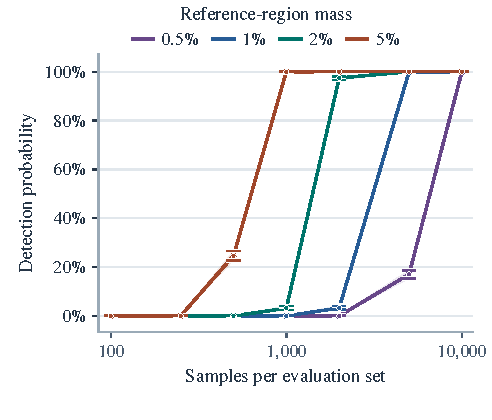
\includegraphics[width=\linewidth]{../figures/support_power_joint.pdf}
\caption{Power to certify complete region removal using the full audit's
$\alpha_{\rm occ}=0.025$, $M=10$, $\rho=0.5$, and eligibility 0.001.
Each point uses 2,000 frozen trials; whiskers and shading show exact 95\%
binomial intervals. Samples per evaluation set are shown on a logarithmic axis.}
\label{fig:support-power}
\end{figure}

\begin{table}[t]
\centering\small
\begin{tabular}{rrr rrrr}
\toprule
Mass & $n$ & & $M=10$ &40&100&440\\
\midrule
1\% &2000&&3.25&0.10&0&0\\
1\% &5000&&99.90&98.90&95.20&73.95\\
2\% &2000&&97.40&80.75&58.75&23.55\\
0.5\% &10000&&99.95&98.60&94.85&72.80\\
\bottomrule
\end{tabular}
\caption{Complete-removal detection probability (\%) as the declared family
grows, reusing the same raw counts. All entries use occupancy error 0.025,
retention 0.5, minimum mass 0.001, and 2,000 trials.}
\label{tab:support-multiplicity}
\end{table}

For a 1\% removed region at $n=5000$, the matched-allocation power is
1998/2000 or 99.9\%; at $n=2000$ it is only 65/2000 or 3.25\%.
For a 2\% region, $n=2000$ gives 1948/2000 or 97.4\%.
The full secondary grid varies retention over $\{0.3,0.5,0.7\}$ and family size
over $\{10,40,100,440\}$, retaining all 2,016 cells.
At the original categorical-only allocation 0.05, exact binomial bounds and
additive Hoeffding bounds use the same four-endpoint Bonferroni construction.
For a 2\% removed region and $n=2000$, exact bounds detect 1981/2000 trials and
Hoeffding detects 0/2000. Both guarantee at least the same nominal family
coverage; their realized conservatism differs. Across the original 336,000
categorical trials, joint interval noncoverage is 3.823\% and one trial falsely
certifies a region whose true retention is at least 0.5. These heterogeneous
pooled rates are descriptive, not substitutes for a per-family guarantee.

Equation~\ref{eq:zerocount} also gives a practical planning limit. Even knowing
a reference mass of 0.1 exactly, observing zero candidate hits needs at least
144 candidate draws for $M=10$, occupancy error 0.025, and retention 0.5.
For 128 prompts, 29 configurations, two representations, three references, and
ten regions, the declared family would require 340 draws per prompt for this
certificate; at 1\% mass it would require 3,470. These are requirements of the specified
conservative certificate, not information-theoretic lower bounds. Eight or
16 seeds per prompt cannot establish rare-region retention under this design.
The T2I policy therefore treats prompt-level point diagnostics as routing
heuristics and validates its population outcomes on independent seeds; it
does not claim prompt-specific deletion absence.

\subsection{Comparison with NDB's regional proportion test}
NDB\cite{richardson2018ndb} compares bin proportions using a pooled two-sided
normal test and reports the fraction of statistically different bins, NDB/$K$.
We prospectively specify a secondary reanalysis of all 336,000 categorical
trials and all 7,200 Gaussian/CIFAR controls. The official implementation is
pinned to commit \texttt{a6bcb4e91198} (full hash in the source manifest); all
3,360,000 categorical per-bin decisions match it exactly. To isolate the
statistical rule, every method receives identical fixed regions and independent
reference/generated evaluation counts. This is an adaptation of NDB's test,
not a comparison with its original pixel representation and training-count fit.
We retain its published per-bin significance 0.05 and add a separate
Bonferroni variant with per-bin significance $0.025/K$.

\begin{table}[t]
\centering\small
\begin{tabular}{rrrrr}
\toprule
$q/p$ & $n$ & NDB & NDB adjusted & Certificate\\
\midrule
1 &1000&4.80&0.10&0\\
0 &1000&99.30&51.55&0\\
0 &2000&100&99.55&3.25\\
0 &5000&100&100&99.90\\
0.5 &5000&83.40&44.55&0\\
\bottomrule
\end{tabular}
\caption{Target-region rejection/certification rates (\%) for reference mass
1\%, ten bins, and 2,000 frozen trials per row. NDB tests equality $q=p$;
the retention certificate establishes $q/p<0.5$. They answer different
questions, so these values do not measure superiority under a common null.}
\label{tab:support-ndb}
\end{table}

Table~\ref{tab:support-ndb} shows NDB's greater sensitivity to smaller changes.
At true retention 0.5, its equality rejection is a correct finding, while a
strictly-below-0.5 certificate should remain unresolved. Under the identical
ten-bin null with a 1\% target and $n=1000$, original mean NDB/$K$ is 0.05215;
the probability of any flagged bin is 40.65\%. The adjusted variant's any-bin
rate is 2.45\%. Original NDB's per-bin level is not a familywise guarantee.
Both NDB variants detect every Gaussian quadrant-removal trial; for the CIFAR
region removal at $n=1000$, both detect 200/200 versus 196/200 retention
certificates. Thus clustering-based loss detection is established prior work;
the audit adds an explicit effect-size resolution and combines its output with
spread, fidelity, and intervention validation. All counts, normalized scores,
Jensen--Shannon divergences, null rates, and trial-proportion intervals appear
in \texttt{ndb\_comparison.json} and its raw arrays. The adjusted normal test
remains approximate, unlike the exact binomial certificate.

\subsection{Representation and partition resolution}
As a secondary robustness analysis, we freeze the complete grid of DINO PCA
dimensions $\{16,32,64\}$ and region counts $K\in\{5,10,20\}$ for five completed
CIFAR configurations. All use the original independent 5,000/5,000/10,000
reference split, 10,000 generated images, seed 1729, and unchanged margins.
The exact occupancy family contains $3(5+10+20)5=525$ regions at
$\alpha_{\rm occ}=0.025$; the support family contains 45 comparisons at
$\alpha_{\rm support}=0.025$. Approximate spread intervals separately use
$0.05/525$. Every configuration has a contraction flag in all nine settings,
no expansion flag, and a passing feature-support gate. Leading DDIM4, Bures4,
fresh leading DDIM2, and covariance-only initialization2 have regional
depletion in all nine settings. UniPC4 has a depletion certificate in seven;
the two exceptions use five regions with 32 or 64 directions. Thus substantial
deficits persist across resolutions, while milder regional findings depend on
the partition. Default-resolution counts and tail rates exactly reproduce the
primary audit, and spread points agree within $7\times10^{-16}$; the revised
family allocation changes no default qualitative flag. All 45 results and
ineligible cells are retained; no primary choice is changed.

\begin{figure*}[t]
\centering
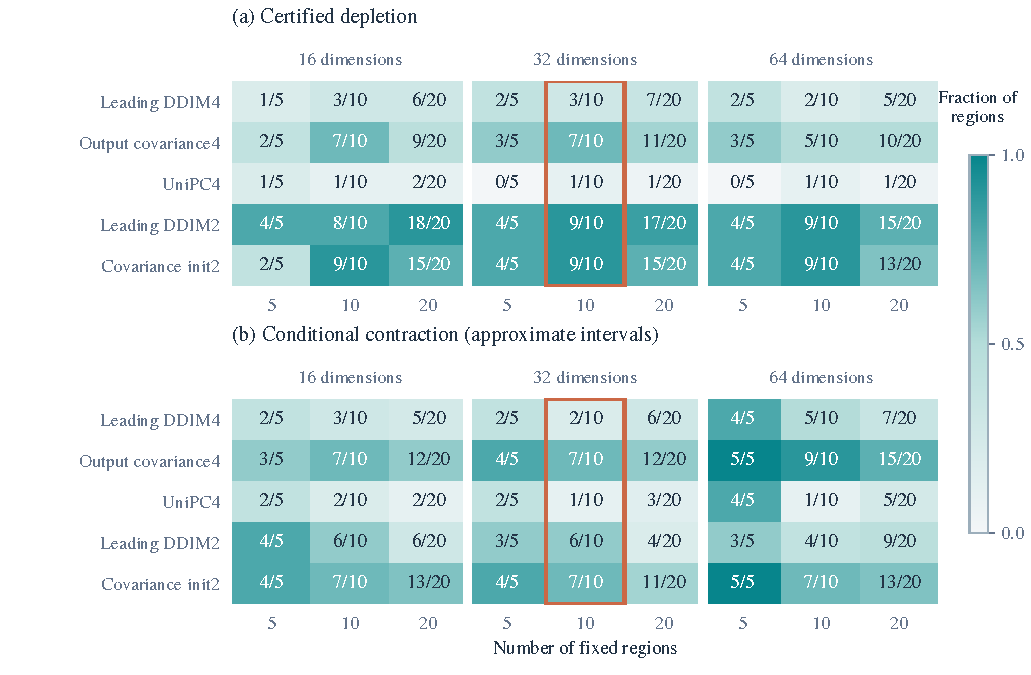
\includegraphics[width=\textwidth]{../figures/support_cifar_resolution.pdf}
\caption{Complete secondary resolution analysis. Entries count flagged regions
out of all $K$ fixed regions; red outlines mark the default 32-direction,
ten-region representation. A region without a spread flag can be unresolved
or have fewer than 30 samples. All 45 support gates pass and no expansion flag
occurs, so the figure displays the two varying outputs. Region identities
change with the resolution; fractions of regions are not fractions of data
probability. Full counts, intervals, eligibility and source hashes accompany
the results.}
\label{fig:support-resolution}
\end{figure*}

\subsection{Interpretation and executable outputs}
The output contains the fixed reference, feature representation, regions,
calibration thresholds, sample counts, ratio intervals, eligibility, unresolved
tests, supported deficit flags, and recommended next comparison. A support
departure is called off-reference expansion only if expansion is independently
supported. The training-comparison branch requires a data reference,
independently validated semantic measurements, a certified data-relative
imbalance (depletion or excess), acceptable resolved-model fidelity, and persistence under
alternative resolved samplers. Otherwise the next step is a controlled sampler
comparison or additional measurement. Invertible contraction can move probability
across a fixed feature boundary; therefore even certified regional depletion
cannot identify a missing semantic mode or unique historical cause.

The practitioner entry point \texttt{audit\_features.py} accepts separate
NPZ fit, calibration, reference-evaluation and candidate arrays, named feature
and sample-ID keys, and a complete frozen configuration. It checks finite
dimensions and declared sample-ID disjointness, records input hashes, and emits
strict JSON measurements and interpretation. External fidelity remains
unmeasured unless supplied explicitly with its evidence source. The delivered
CIFAR example reproduces the original regional intervals and support gate;
synthetic interface checks reject overlapping IDs and invalid evidence.

The complete controlled validation takes 276 seconds on CPU with one BLAS
thread and no GPU. Run \texttt{support\_validate.py --run}, followed by
the supplied secondary-analysis and plotting scripts. These scripts preserve
the frozen raw trials, record source and output hashes, and regenerate editable
vector figures. External fidelity and learned-model intervention outcomes
are reported in their respective experiments rather than inferred from these
feature controls.

\subsection{Two-sided mass balance with shared reference uncertainty}
\label{sec:support-mass-balance}
Severe relative depletion and useful mass balance ask different questions.
For a fixed semantic region, let $p_j$ and $q_{aj}$ be its probabilities under
data and candidate~$a$, respectively, using all images as the denominator.
A candidate can retain a class while allocating too much probability to it.
We therefore also use a prespecified absolute balance tolerance~$\delta$.
This complements the relative-depletion test: a region of mass at most
$\delta$ can disappear without violating an absolute tolerance.

Suppose the study declares $R$ distinct reference-region intervals and $C$
candidate-region intervals. Allocate fraction $w$ of total error $\alpha$ to
the reference. The Clopper--Pearson intervals~\cite{clopper1934confidence}
$[p_j^-,p_j^+]$ have each tail $\alpha w/(2R)$, and
$[q_{aj}^-,q_{aj}^+]$ have each tail $\alpha(1-w)/(2C)$.
A union bound gives simultaneous coverage at least $1-\alpha$ for all
declared masses. On that event,
\begin{equation}
q_{aj}-p_j\in I_{aj}
=[q_{aj}^- -p_j^+,\ q_{aj}^+-p_j^-].
\label{eq:supp_shared_mass_difference}
\end{equation}
Charging each shared reference interval once avoids a redundant multiplicity
penalty. Independence between candidates or between regions is unnecessary;
independent evaluation rows within each fixed population remain required.
This guarantee conditions on the trained models and fixed measurement functions.

We certify excess if $\inf I_{aj}>\delta$, depletion if
$\sup I_{aj}<-\delta$, and equivalence if
$I_{aj}\subseteq[-\delta,\delta]$; all remaining cases are inconclusive.
All-class equivalence requires every interval to be contained. Persistent
imbalance requires the same class and direction under all declared resolved
samplers, with every sampler fidelity-qualified. Certified balance requires
all-class equivalence and fidelity qualification under every probe. Mixed
directions are retained; inconclusive outcomes do not imply a numerical-only
cause. These are operational statements, not identification of a unique cause.
When data representativeness is an objective and validated data regions are
available, the data audit is performed regardless of teacher-relative flags.
A teacher and all its samplers can share the same imbalance; agreement with
the teacher alone cannot establish data-relative balance.

The separately frozen MNIST balance follow-up uses $\alpha=.025$, $w=1/2$,
$R=10$, $C=360$, and $\delta=.03$, with complete $.02/.04$ sensitivity.
The margin is three percentage points of unconditional mass, approximately
30\% of a nominal balanced digit class; it is domain-specific. All 10,000 real
test images are available for semantic counts because classifiers and their
threshold were fixed using training data. Geometry retains its independent
fit/calibration/evaluation pools. Rejection remains a separate fidelity event.

Sample size was chosen before fresh follow-up training from 20,000 synthetic
multinomial trials per setting, using the old reference proportions. With
16,000 generated and 10,000 reference images, excess at $q_3=.16$ versus
$p_3=.0983$ is certified in 99.23\% of trials
(95\% Monte Carlo interval: 99.10--99.35\%); reference-matched masses yield
all-class equivalence in 95.58\% (95.29--95.86\%). With $q_3=.087$, all-class
equivalence remains only 45.12\% (44.42--45.81\%). Thus the design permits
meaningful inconclusive outcomes rather than relaxing the tolerance to obtain
a pass. Complete grids include 5,000/10,000 reference images and
8,000/16,000/32,000/64,000 generated images.

The reusable \texttt{diagnostic\_mass\_balance.py} API and counts-JSON CLI
implement these rules. The study wrapper verifies all 36 diagnosis artifacts
and freezes every label before independent outcome generation. The original
relative-depletion API and its recorded results remain unchanged. Paired
fidelity and separate support families receive errors $.0125$ each, so their
union with the mass family is bounded by $.05$. Full-data self-comparisons are
explicit structural identity anchors, not evidence of absolute visual fidelity.
The joint statement averages over the sampled real-reference pools, conditional
on the trained generators and frozen classifiers. Semantic bounds use all
10,000 reference rows and are not additionally conditioned on the realized
geometry-fit subset. Geometry-based bounds condition on their independent
fitting pools and then average over them; the union bound does not require
independence between these families.

\section{Gaussian initialization--integration identity}
\label{supp:gaussian}
For a centered clean Gaussian coordinate with variance $\lambda>0$, isotropic
variance-preserving noising gives variance $v_t=\bar\alpha_t\lambda+1-\bar\alpha_t$
at timestep $t$, where $\bar\alpha_t$ is the cumulative signal coefficient.
For a value $x_t$ of the noisy coordinate, the exact noise predictor is
$\epsilon^*(x_t,t)=\sqrt{1-\bar\alpha_t}\,x_t/v_t$.
Substituting into deterministic DDIM without clipping gives the multiplier
from timestep $t$ to an earlier timestep $s$:
\begin{equation}
m_{st}=\frac{\sqrt{\bar\alpha_s\bar\alpha_t}\lambda+
\sqrt{(1-\bar\alpha_s)(1-\bar\alpha_t)}}{v_t}.
\label{eq:supp_ddim_step}
\end{equation}
With $u_t=(\sqrt{\bar\alpha_t\lambda},\sqrt{1-\bar\alpha_t})$,
the numerator is $u_s^\top u_t$ and $\|u_t\|^2=v_t$. Thus
$m_{st}=\sqrt{v_s/v_t}\cos\angle(u_s,u_t)$.
Multiplying adjacent grid transitions telescopes the variance factors.
Let $\nu_{\rm start}$ be the actual initial variance, $v_{\rm start}$ and
$v_{\rm end}$ the noising variances at the grid endpoints, and
$X_{\rm out}$ the output coordinate.
\begin{equation}
\frac{\operatorname{Var}(X_{\rm out})}{\lambda}
=\frac{\nu_{\rm start}}{v_{\rm start}}
\frac{v_{\rm end}}{\lambda}
\prod_{t\rightarrow s}\cos^2\angle(u_s,u_t).
\label{eq:supp_ddim_variance}
\end{equation}
The clean endpoint has $v_{\rm end}=\lambda$.
Matched noisy-marginal initialization sets $\nu_{\rm start}=v_{\rm start}$;
standard-normal initialization sets $\nu_{\rm start}=1$.
The numerical oracle uses the checkpoint's actual alpha values and the
scheduler's actual previous-timestep arithmetic. Learned samples keep the
checkpoint's standard clipping behavior, so the exact Gaussian identity is a
surrogate prediction, not an equality asserted for those samples.

For a fixed start and endpoint and ordered angles in the first quadrant,
splitting an angular interval reduces the product-of-cosines deficit because
$\cos a\cos b\geq\cos(a+b)$ for $a,b\geq0$ with $a+b\leq\pi/2$.
This refinement statement does not apply when a changed step count also changes
the initial timestep, when clipping is active, or when the learned dynamics
are nonlinear or noncommuting. Our intermediate-state measurements report
projected off-diagonal mixing and regression residuals to assess these limits.
We do not use a Gaussian integration rule in a covariance-dependent time
coordinate as evidence for a learned-model solver's universal order.

\section{A straight-interpolation flow-matching oracle}
\label{supp:flow_oracle}

\begin{figure*}[t]
\centering
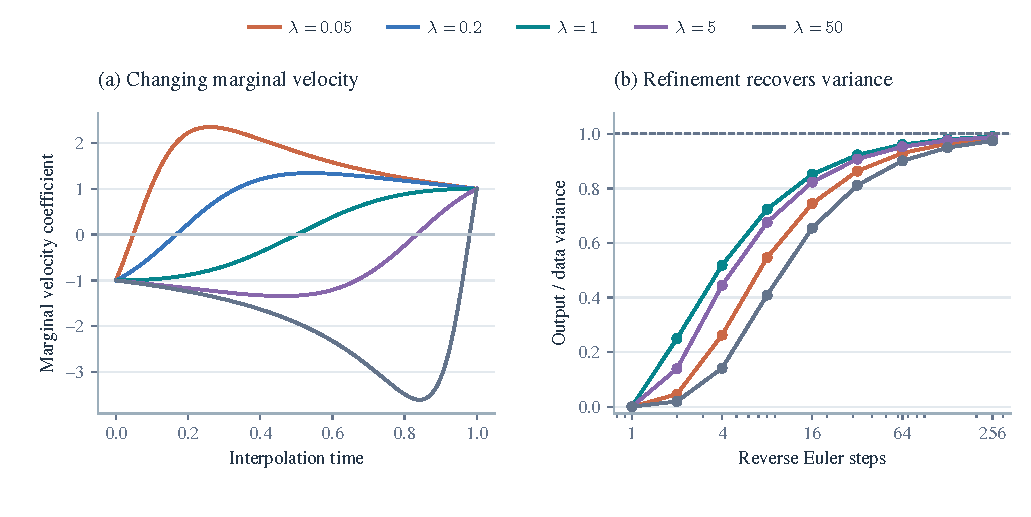
\includegraphics[width=\textwidth]{../figures/theory_flow.pdf}
\caption{Straight-interpolation Gaussian flow oracle. The population regression
velocity coefficient varies with time even though each endpoint-conditioned
path has a constant velocity. Reverse Euler sampling contracts the output
variance on the complete noise-to-data interval, and refinement approaches
the exact variance. Both panels show exact Gaussian-oracle predictions.}
\label{fig:flow_oracle}
\end{figure*}

A Gaussian oracle connects the same variance diagnostic to
straight-interpolation flow matching~\cite{lipman2023flow,liu2023rectified}.
To distinguish per-pair paths from the marginal sampling dynamics,
let $X_0\sim\mathcal N(0,\lambda)$ and $Z\sim\mathcal N(0,1)$ be independent,
with $\lambda>0$. For $t\in[0,1]$ from data to noise, define the
interpolated coordinate $X_t$ and its variance $v_t$:
\begin{equation}
X_t=(1-t)X_0+tZ,\qquad v_t=(1-t)^2\lambda+t^2.
\label{eq:fm_interpolation}
\end{equation}
The per-pair interpolation velocity $Z-X_0$ is constant. The population
regression field used by the marginal ODE at state $x$ is $b_t x$:
\begin{equation}
\mathbb E[Z-X_0\mid X_t=x]
=\frac{t-(1-t)\lambda}{v_t}x=b_tx.
\label{eq:fm_gaussian_velocity}
\end{equation}
This follows from Gaussian conditional expectation and
$\operatorname{Cov}(Z-X_0,X_t)=t-(1-t)\lambda$.
Because $b_t=\tfrac12\partial_t\log v_t$, exact ODE evolution from $t$ to $s$
maps $x_t$ to $\sqrt{v_s/v_t}\,x_t$. In particular, noise at $t=1$ reaches
variance $\lambda$ at $t=0$.

\paragraph{The measured variance ratio under Euler sampling.}
A reverse Euler step from $t$ to an earlier $s$ on a fixed descending grid multiplies a coordinate by
$m_{st}=1+(s-t)b_t$. Define
$u_t=((1-t)\sqrt\lambda,t)$, so that $v_t=\|u_t\|^2$. Since $u_t$ is affine,
\begin{equation}
m_{st}=\frac{u_s^\top u_t}{v_t}
=\sqrt{\frac{v_s}{v_t}}\cos\angle(u_s,u_t).
\label{eq:fm_euler_step}
\end{equation}
Let $X_{\rm out}$ be the final coordinate at $t=0$. Starting at $t=1$
with unit variance gives
\begin{equation}
\frac{\operatorname{Var}(X_{\rm out})}{\lambda}
=\prod_{t\rightarrow s}\cos^2\angle(u_s,u_t).
\label{eq:fm_variance_ratio}
\end{equation}
This is the same operational variance-ratio quantity as the Gaussian diffusion
calculation, derived here for explicit Euler on a different probability path.
For monotone grids spanning the fixed endpoints, the factors lie in $[0,1]$.
Refining an interval replaces $\cos^2(a+b)$ with
$\cos^2a\cos^2b$, which is no smaller for $a,b\geq0$, $a+b\leq\pi/2$.
The ratio converges to one as the maximum grid spacing vanishes.
At a truncated start with actual variance $\nu_{\rm start}$, an additional
factor $\nu_{\rm start}/v_{\rm start}$ appears, separating initialization from
integration as before.

For $\lambda=1$, four uniform reverse steps have multipliers
$(0.75,0.8,1,1.2)$, product $0.72$, and output variance $0.5184$.
A single full-interval Euler step has multiplier zero for every $\lambda>0$,
despite the straight per-pair interpolation paths. The supplied oracle script
checks five eigenvalues and nine grid sizes, and independently simulates
200,000 Gaussian samples for selected grids. It verifies the factorization
and monotone refinement numerically.

The oracle assumes independent Gaussian endpoints and an exact regression field.
Coupling is consequential: if instead $X_0=\sqrt\lambda Z$, one reverse Euler
step has multiplier $\sqrt\lambda$ and is exact. Straightness alone therefore
does not determine the sampling error; the marginal regression and endpoint
coupling matter. This is consistent with rectified flow's use of a changed
coupling to straighten marginal trajectories\cite{liu2023rectified}.
We use this elementary calculation to explain a measurable failure mode.
For learned flows, the empirical support, fidelity, and intervention checks
determine whether these effects predict useful repairs.


\section{Initialization and numerical repair on CIFAR-10}
\label{supp:cifar}

\subsection{Checkpoint, references, and evaluation units}
The checkpoint is \texttt{google/ddpm-cifar10-32}, revision
\texttt{267b167dc01f0e4e6192\allowbreak{}3ea244e8b988f84deb80}. We retain its standard
epsilon prediction, variance schedule, and clipping configuration.
DINOv2-base~\cite{oquab2024dinov2} uses revision
\texttt{f9e44c814b77203eaa57\allowbreak{}a6bdbbd535f21ede1415}; Inception uses the standard
\texttt{pytorch-fid} weights. Features are deterministic. DINO inputs are
bilinearly resized to $224\times224$, normalized with ImageNet mean and
standard deviation, and represented by the final CLS token. The cached
teacher features use the identical preprocessing.

Teacher images 0--4,999 fit PCA, regions, initial moments, and support geometry;
5,000--9,999 calibrate tails; 10,000--19,999 evaluate. The real reference is
the 10,000-image CIFAR-10 test split. Reusing these fixed benchmark references
from pilot to final evaluation means that the held-out component is the
generated seed set, not previously unseen real data. Each panel uses disjoint,
equally sized teacher and real-reference rows. All arms within a study share
generated seeds and reference panels. No bootstrap duplicates enter nearest
neighbor metrics or KID. Uncertainty is conditional on the fixed benchmark
references and summarizes five independent generated panels.

Global variance ratios use the first 128 unwhitened teacher-fit PCA coordinates
in pixels and DINO features. Regional spread uses 32 unwhitened PCA coordinates;
region assignments and support distances use their whitened coordinates.
PRDC~\cite{naeem2020density} uses $k=5$ and all 768 DINO coordinates. KID~\cite{binkowski2018demystifying} is the
unbiased degree-three polynomial-kernel statistic on 2,048-dimensional standard
Inception features, computed over each full panel in float64. FID~\cite{heusel2017gans} is computed
on all 10,000 generated and 10,000 real samples; it is reported without a
confidence interval. Means and 95\% Student-$t$ intervals use the five panels;
contrasts pair the same panels. These intervals do not quantify uncertainty
over checkpoints, datasets, or unseen prompt populations.

\subsection{Frozen studies and executable interventions}
The development seed range begins at 160010, the original final range at 260010,
the trajectory control at 360010, the reference check at 460010, and independent
initializer confirmation at 660010. A separate generator per image makes the
noise seed independent of batching. Timestamped protocols and amendments were
written before their corresponding final outcomes. The 22-arm primary study
includes leading/trailing DDIM, stochastic trailing DDIM with $\eta=1$,
DPM++2M, UniPC, initial-moment correction, and output-moment correction.
The two-step DPM++/UniPC comparisons were added before their final measurements.
The CAS comparison, mean/covariance ablation, and fresh covariance-only
confirmation are separate recorded studies. Every arm is retained below.

At $K=2,4,8$ denoiser calls, trailing DDIM, DPM++2M, and UniPC use identical timestep grids,
for example $[999,749,499,249]$ at four steps. Leading grids start at 500,750,
and 875 respectively and therefore change both initialization and integration
when the budget changes. Official scheduler prediction transforms and clipping
are retained; practical solver differences are not attributed solely to order.

Let $U\in\mathbb R^{3072\times128}$ contain 128 orthonormal teacher-fit
pixel components and $\widehat\lambda\in\mathbb R^{128}$ their sample
variances. Let $I$ be the pixel-space identity and
$\widehat\sigma^2_\perp$ the remaining variance divided by $3072-128$.
The clean covariance estimate is
\begin{equation}
\widehat C=U\operatorname{diag}(\widehat\lambda)U^\top
+\widehat\sigma^2_\perp(I-UU^\top),
\label{eq:supp_cifar_covariance}
\end{equation}
For standard Gaussian noise $Z\sim\mathcal N(0,I)$, the centered remedy initializes
$[(1-\bar\alpha_{\rm start})I+\bar\alpha_{\rm start}\widehat C]^{1/2}Z$,
where $\bar\alpha_{\rm start}$ is the cumulative signal coefficient at the first timestep.
The full-moment variant additionally adds
$\sqrt{\bar\alpha_{\rm start}}\widehat\mu$, where $\widehat\mu$ is the
teacher-fit pixel mean. The mean-only ablation adds this term to unscaled
$Z$. None requires an additional denoiser call.

Output restoration fits a Gaussian Bures map in 64 teacher-fit pixel PCA
coordinates using only the pilot leading-DDIM outputs. If $C_s,C_r$ are
their source and reference covariances, the map is
$A=C_s^{-1/2}(C_s^{1/2}C_rC_s^{1/2})^{1/2}C_s^{-1/2}$.
It maps projected means and covariances, preserves the orthogonal residual,
and clips final pixels to the valid range. Map parameters are frozen before
final evaluation. It adds no denoiser calls; clipping affects approximately
3.0\% of pixel coordinates at four steps. At four calls, this control raises the pixel variance ratio from 0.376 to
0.917 while lowering real-data coverage from 0.478 to 0.332 and worsening
KID from 0.0903 to 0.1024. UniPC at the same four-call budget reaches
coverage 0.549 and KID 0.0694. The outcome comparison separates restored
pixel spread from improved fidelity and coverage.

% BEGIN AUTO ALLARMS
\begin{table*}[t]
\centering
\small
\setlength{\tabcolsep}{3.5pt}
\caption{Complete original primary (P), CAS (C), and initializer-ablation (A) comparisons, each with 10,000 generated images. VR is teacher-relative variance ratio; precision/coverage use real-data DINO features. KID intervals summarize five 2,000-image panels. Calls count forwards plus JVPs for CAS (3/7 within 4/8 ceilings). Bures reuses the corresponding DDIM outputs; its denoiser cost is that source cost and its extra transformation time is not recorded. Wall time is shared-device generation time in seconds. Full intervals for every metric are in the machine-readable results.}
\label{tab:cifar_allarms}
\begin{tabular}{llrrrrrrr}
\toprule
Method & Calls & FID$\downarrow$ & Pixel VR & DINO VR & Prec.$\uparrow$ & Cov.$\uparrow$ & KID$\times10^3\downarrow$ & Sec. \\
\midrule
P: Initial mean+cov. & 1 & 285.0 & 0.929 & 0.128 & 0.938 & 0.091 & $306.8\pm1.8$ & 3.3 \\
P: DDIM leading & 1 & 450.9 & 0.109 & 0.016 & 0.001 & 0.000 & $585.5\pm3.3$ & 7.5 \\
P: DDIM trailing & 1 & 319.9 & 0.250 & 0.083 & 0.552 & 0.022 & $347.6\pm1.1$ & 3.7 \\
A: Initial cov. & 2 & 138.8 & 0.653 & 0.411 & 0.968 & 0.298 & $126.1\pm2.1$ & 20.4 \\
A: Initial mean & 2 & 188.4 & 0.106 & 0.296 & 0.960 & 0.205 & $205.4\pm1.7$ & 27.4 \\
P: DPM++2M & 2 & 242.8 & 0.266 & 0.283 & 0.608 & 0.108 & $223.2\pm2.9$ & 17.4 \\
P: Initial mean+cov. & 2 & 146.4 & 0.631 & 0.422 & 0.963 & 0.297 & $141.3\pm2.2$ & 7.1 \\
P: DDIM leading & 2 & 182.2 & 0.109 & 0.281 & 0.969 & 0.203 & $185.3\pm1.8$ & 7.1 \\
P: DDIM trailing & 2 & 216.3 & 0.198 & 0.288 & 0.797 & 0.131 & $192.2\pm2.6$ & 7.1 \\
P: UniPC & 2 & 242.8 & 0.266 & 0.283 & 0.608 & 0.108 & $223.2\pm2.9$ & 15.2 \\
C: CAS & 3 & 282.7 & 0.357 & 0.130 & 0.788 & 0.077 & $290.2\pm3.2$ & 107.1 \\
P: Output Bures & 4 & 111.1 & 0.917 & 0.515 & 0.966 & 0.332 & $102.4\pm1.6$ & --- \\
P: DPM++2M & 4 & 80.1 & 0.599 & 0.733 & 0.918 & 0.526 & $77.4\pm2.7$ & 11.7 \\
P: DDIM $\eta=1$ & 4 & 149.1 & 0.207 & 0.547 & 0.911 & 0.327 & $161.6\pm4.4$ & 14.1 \\
P: Initial mean+cov. & 4 & 89.7 & 0.473 & 0.686 & 0.932 & 0.488 & $92.6\pm2.4$ & 13.7 \\
P: DDIM leading & 4 & 87.9 & 0.376 & 0.677 & 0.935 & 0.478 & $90.3\pm2.5$ & 13.9 \\
P: DDIM trailing & 4 & 111.2 & 0.371 & 0.638 & 0.911 & 0.428 & $113.2\pm4.2$ & 12.1 \\
P: UniPC & 4 & 73.1 & 0.671 & 0.758 & 0.913 & 0.549 & $69.4\pm2.6$ & 13.6 \\
C: CAS & 7 & 217.3 & 0.661 & 0.309 & 0.961 & 0.227 & $243.3\pm5.5$ & 220.9 \\
P: Output Bures & 8 & 56.4 & 0.949 & 0.812 & 0.927 & 0.596 & $50.5\pm1.8$ & --- \\
P: DPM++2M & 8 & 32.5 & 0.943 & 0.975 & 0.859 & 0.731 & $26.4\pm1.2$ & 23.7 \\
P: DDIM $\eta=1$ & 8 & 74.3 & 0.387 & 0.825 & 0.906 & 0.564 & $71.2\pm2.9$ & 36.2 \\
P: Initial mean+cov. & 8 & 42.6 & 0.633 & 0.913 & 0.892 & 0.676 & $37.8\pm2.2$ & 41.5 \\
P: DDIM leading & 8 & 41.0 & 0.624 & 0.915 & 0.893 & 0.680 & $36.3\pm2.1$ & 24.5 \\
P: DDIM trailing & 8 & 48.3 & 0.606 & 0.903 & 0.879 & 0.649 & $43.5\pm2.3$ & 25.7 \\
P: UniPC & 8 & 31.3 & 1.020 & 0.986 & 0.849 & 0.740 & $24.5\pm1.1$ & 34.5 \\
\bottomrule
\end{tabular}
\end{table*}
% END AUTO ALLARMS

\subsection{Covariance initialization improves two-call fidelity and coverage}
\label{supp:cifar_initializer}
Covariance-only initialization reduces two-call KID from 0.1858 to 0.1264
(32.0\%) in the separate fresh confirmation, while real-data DINO coverage
increases from 0.206 to 0.288. These are five paired generated panels from
one fixed pretrained checkpoint. The earlier secondary ablation isolates
mean and covariance using the original paired seeds: its KID values are
0.1261 for covariance, 0.1413 for full moments, and 0.2054 for mean only.
That analysis motivated the separately predeclared fresh-sample study;
the original frozen selector and all earlier outcomes remain unchanged. The primary confirmation
criterion is lower real-data KID against each of the five declared alternatives;
all other metrics remain reported. Table~\ref{tab:cifar_v2_contrasts} gives
complete paired contrasts and simultaneous intervals. Coverage is similar
between the two covariance variants, so the mean-term finding concerns KID,
not an improvement in every metric.

% BEGIN AUTO V2CONTRASTS
\begin{table*}[t]
\centering
\small
\setlength{\tabcolsep}{3.5pt}
\caption{All five prespecified fresh-confirmation contrasts: centered covariance initializer minus comparator. KID intervals simultaneously cover the five comparisons at 95\% by Bonferroni adjustment; coverage intervals are ordinary paired 95\% intervals. Negative KID and positive coverage differences favor the centered initializer.}
\label{tab:cifar_v2_contrasts}
\begin{tabular}{lrrrr}
\toprule
Comparator & $\Delta$KID$\times10^3$ & Simultaneous interval & $\Delta$coverage & Paired interval \\
\midrule
DDIM leading & -59.38 & [-61.38,-57.39] & 0.0821 & [0.0672,0.0970] \\
DDIM trailing & -65.90 & [-70.11,-61.69] & 0.1575 & [0.1501,0.1649] \\
DPM++2M & -96.14 & [-100.61,-91.66] & 0.1820 & [0.1714,0.1926] \\
UniPC & -96.14 & [-100.61,-91.66] & 0.1820 & [0.1714,0.1926] \\
Initial mean+cov. & -14.11 & [-17.90,-10.31] & -0.0012 & [-0.0157,0.0133] \\
\bottomrule
\end{tabular}
\end{table*}
% END AUTO V2CONTRASTS

\begin{figure}[t]
\centering
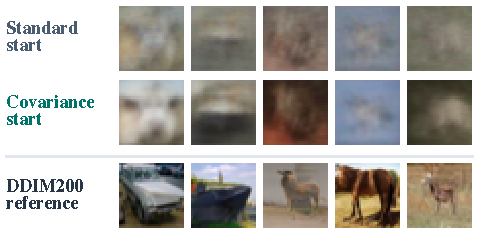
\includegraphics[width=\linewidth]{../figures/initializer_examples.pdf}
\caption{Fixed-index examples from the two-call standard-normal and
covariance-start arms. The two upper rows are paired by initial noise seed,
using the eighth image of each saved 2,000-image panel. The separately
seeded DDIM200 row uses the eighth image of each 400-image reference
panel and provides a visual reference. Every selected image is displayed.}
\label{fig:initializer_examples}
\end{figure}

\subsection{The same outputs improve under an untouched external reference}
\label{supp:cifar101}
The unchanged covariance-initialized outputs reduce KID by 32.7\% against
untouched CIFAR-10.1v6. This separate reference evaluation was frozen
before downloading or scoring CIFAR-10.1v6~\cite{recht2018cifar10}.
The official release supplies
2,000 images, exactly 200 per class, sampled separately for testing CIFAR-10
generalization. We pin repository commit
\texttt{d9982abb0bfc4846b8d1\allowbreak{}3a11e66b887d946205d0}, preserve file hashes,
and verify shapes, class counts, and absence of exact pixel duplicates with
the original CIFAR-10 test reference. This is a new reference for our method
development; it does not assert that general-purpose pretrained representations
have never encountered related public images.

Every available 10,000-image confirmatory candidate is included: 22 primary
arms, two CAS arms, two initializer ablations, and six fresh initializer arms.
Generated images, seeds, features, methods, and selections remain unchanged.
The same frozen Inception and DINO extraction pipeline embeds the new real
reference. Each arm's five disjoint 2,000-image generated panels is compared
to all 2,000 external reference images. Consequently, Student-$t$ intervals
condition on this shared real reference. Four prespecified paired KID contrasts
receive Bonferroni 98.75\% marginal intervals, giving simultaneous 95\%
coverage for that four-comparison family under the panel-effect approximation.
Precision and coverage intervals are descriptive. We do not use bootstrapped
image duplicates in nearest-neighbor metrics.

All four predicted KID directions hold (Fig.~\ref{fig:cifar101}). Output
covariance restoration at four calls worsens KID by 0.01070 [0.00843,0.01297]
and decreases coverage by 0.1269, despite increasing precision by 0.0262.
UniPC4 improves KID by 0.02182 [0.02015,0.02348] and coverage by 0.0564,
with a 0.0228 precision decrease. In the fresh two-call confirmation,
centered initialization reduces KID from 0.19060 to 0.12832, a 32.7\%
reduction; its paired difference is $-0.06228$ [$-0.06422,-0.06035$].
Coverage rises from 0.3221 to 0.4268 (difference 0.1047 [0.0895,0.1199]),
while precision decreases from 0.9756 to 0.9580. Compared with mean-plus-covariance
initialization, centered initialization improves KID by 0.01272
[0.00896,0.01647]; its coverage difference is $-0.0072$
[$-0.0198,0.0054$]. Thus the external reference supports both the useful
initialization repair and the failure of output-moment restoration, while
retaining the observed fidelity--coverage tradeoffs.

No additional denoiser samples are generated. DINO and Inception extraction
of the 2,000 new images takes 8.6 and 53.0 recorded seconds on shared hardware;
all 32-arm metric evaluation takes 9.4 seconds. The artifact manifest records
reference and feature hashes, the frozen protocol, source hashes, resource
use, and every primary comparison. Table~\ref{tab:cifar101_all} retains every
arm, including unfavorable CAS and initializer comparisons.

\begin{figure*}[t]
\centering
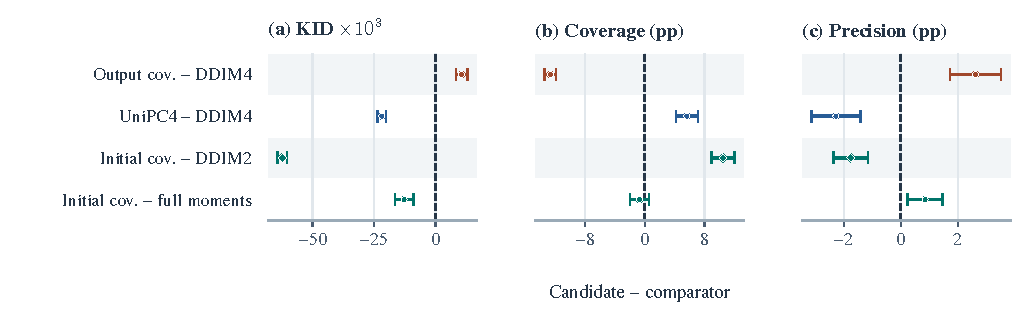
\includegraphics[width=\textwidth]{../figures/cifar101_confirmation.pdf}
\caption{Untouched CIFAR-10.1v6 confirmation using unchanged generated samples.
Four prespecified contrasts are shown. KID intervals have the four-comparison
adjustment; coverage and precision use ordinary 95\% intervals. All intervals
condition on the fixed external real reference. Opposing precision and
coverage changes reinforce the need for multiple measurements.}
\label{fig:cifar101}
\end{figure*}
\begin{table*}[t]
\centering\footnotesize
\setlength{\tabcolsep}{4pt}
\caption{Untouched CIFAR-10.1v6 reference evaluation. All 32 frozen candidate arms are retained. Mean $\pm$95\% interval over five independent generated panels, conditional on the same fixed 2,000-image external reference. DINO precision and coverage are descriptive. P/C/A/V2 denote primary/CAS/initializer ablation/fresh initializer confirmation.}
\label{tab:cifar101_all}
\begin{tabular}{llrrr}
\toprule
Study & Arm & KID$\times10^3\downarrow$ & Precision$\uparrow$ & Coverage$\uparrow$ \\
\midrule
P & Output covariance 4 & $100.825\pm0.422$ & $0.948\pm0.002$ & $0.481\pm0.005$ \\
P & Output covariance 8 & $48.546\pm0.898$ & $0.909\pm0.007$ & $0.715\pm0.014$ \\
P & DPM++ 2 & $232.929\pm3.237$ & $0.614\pm0.016$ & $0.154\pm0.024$ \\
P & DPM++ 4 & $76.362\pm1.481$ & $0.904\pm0.006$ & $0.646\pm0.014$ \\
P & DPM++ 8 & $25.346\pm0.446$ & $0.852\pm0.008$ & $0.790\pm0.010$ \\
P & Stochastic DDIM 4 & $163.798\pm2.586$ & $0.864\pm0.007$ & $0.446\pm0.024$ \\
P & Stochastic DDIM 8 & $72.596\pm2.015$ & $0.884\pm0.011$ & $0.653\pm0.012$ \\
P & Initial mean+cov. 1 & $316.809\pm1.891$ & $0.973\pm0.004$ & $0.132\pm0.007$ \\
P & Initial mean+cov. 2 & $141.748\pm1.833$ & $0.949\pm0.006$ & $0.437\pm0.014$ \\
P & Initial mean+cov. 4 & $92.056\pm1.769$ & $0.919\pm0.009$ & $0.619\pm0.012$ \\
P & Initial mean+cov. 8 & $36.878\pm0.972$ & $0.881\pm0.007$ & $0.761\pm0.016$ \\
P & Leading DDIM 1 & $595.636\pm2.339$ & $0.000\pm0.000$ & $0.000\pm0.000$ \\
P & Leading DDIM 2 & $189.848\pm2.061$ & $0.979\pm0.005$ & $0.322\pm0.020$ \\
P & Leading DDIM 4 & $90.125\pm1.802$ & $0.922\pm0.008$ & $0.608\pm0.011$ \\
P & Leading DDIM 8 & $35.464\pm1.075$ & $0.884\pm0.013$ & $0.763\pm0.015$ \\
P & Trailing DDIM 1 & $353.858\pm1.587$ & $0.390\pm0.017$ & $0.022\pm0.009$ \\
P & Trailing DDIM 2 & $199.990\pm2.138$ & $0.791\pm0.016$ & $0.195\pm0.012$ \\
P & Trailing DDIM 4 & $113.551\pm3.041$ & $0.876\pm0.007$ & $0.569\pm0.017$ \\
P & Trailing DDIM 8 & $42.641\pm1.168$ & $0.869\pm0.008$ & $0.741\pm0.018$ \\
P & UniPC 2 & $232.929\pm3.237$ & $0.614\pm0.016$ & $0.154\pm0.024$ \\
P & UniPC 4 & $68.309\pm1.436$ & $0.899\pm0.005$ & $0.665\pm0.014$ \\
P & UniPC 8 & $23.633\pm0.536$ & $0.845\pm0.014$ & $0.790\pm0.009$ \\
C & CAS ceiling 4 & $297.637\pm2.479$ & $0.753\pm0.011$ & $0.107\pm0.010$ \\
C & CAS ceiling 8 & $246.371\pm5.967$ & $0.971\pm0.005$ & $0.357\pm0.007$ \\
A & Initial covariance 2 & $127.881\pm1.205$ & $0.959\pm0.005$ & $0.433\pm0.015$ \\
A & Initial mean 2 & $207.572\pm1.883$ & $0.962\pm0.003$ & $0.331\pm0.012$ \\
V2 & DPM++ 2 & $232.202\pm1.627$ & $0.614\pm0.006$ & $0.152\pm0.010$ \\
V2 & Initial covariance 2 & $128.321\pm1.914$ & $0.958\pm0.007$ & $0.427\pm0.012$ \\
V2 & Initial mean+cov. 2 & $141.036\pm2.629$ & $0.950\pm0.004$ & $0.434\pm0.013$ \\
V2 & Leading DDIM 2 & $190.602\pm2.626$ & $0.976\pm0.002$ & $0.322\pm0.011$ \\
V2 & Trailing DDIM 2 & $200.159\pm2.041$ & $0.788\pm0.019$ & $0.188\pm0.006$ \\
V2 & UniPC 2 & $232.202\pm1.627$ & $0.614\pm0.006$ & $0.152\pm0.010$ \\
\bottomrule
\end{tabular}
\end{table*}


\subsection{Frozen selectors and threshold sensitivity}
% BEGIN AUTO SELECTORS
\begin{table}[t]
\centering
\small
\setlength{\tabcolsep}{3.5pt}
\caption{Frozen pilot choices evaluated on fresh generated panels. Metrics average budgets 2/4/8 within each panel, followed by the five-panel interval. The later centered-initializer confirmation is separate.}
\label{tab:cifar_selection}
\begin{tabular}{lcc}
\toprule
Selection rule & KID$\times10^3\downarrow$ & Coverage$\uparrow$ \\
\midrule
Default DDIM & $103.9\pm1.7$ & $0.453\pm0.016$ \\
Fixed DPM++ & $109.0\pm2.2$ & $0.455\pm0.011$ \\
Fixed UniPC & $105.7\pm2.1$ & $0.466\pm0.012$ \\
Variance only & $89.4\pm1.5$ & $0.456\pm0.010$ \\
Precision only & $94.0\pm2.0$ & $0.457\pm0.020$ \\
PRDC harmonic & $87.1\pm2.1$ & $0.481\pm0.019$ \\
Vendi & $78.4\pm1.8$ & $0.529\pm0.013$ \\
Teacher Fr\'echet & $78.4\pm1.8$ & $0.529\pm0.013$ \\
Audit (frozen v1) & $79.0\pm1.9$ & $0.526\pm0.015$ \\
\bottomrule
\end{tabular}
\end{table}
% END AUTO SELECTORS
The pilot audit first computes the Gaussian initialization penalty
$1-V_{\rm practical}/V_{\rm matched}$. Above 0.5 it selects initial-moment
correction. Otherwise it considers DPM++2M and UniPC on the matched trailing
grid, retaining candidates whose teacher precision is at least the
leading-DDIM precision minus 0.05, and maximizes teacher coverage. If neither
passes, it retains leading DDIM. These decisions are full moments at two calls,
UniPC at four, and DPM++ at eight; the later centered initializer does not
silently replace the original two-call choice.

The competing selectors maximize pixel variance, teacher precision, the harmonic
mean of teacher precision and coverage, or cosine-kernel Vendi, or minimize
teacher-DINO Fr\'echet distance. Vendi uses the entropy of the normalized
uncentered cosine-kernel spectrum. Fixed DPM++ and UniPC always choose that
solver. Every selector sees only pilot generated samples. The fixed benchmark
reference is shared. The audit evaluates a restricted diagnostic shortlist;
the results establish useful choices but not an optimal search policy or
a universal reduction in required diagnostic compute.

Sensitivity is reported without changing final selections. Initialization
penalty thresholds 0.25,0.5,0.75 all route only the two-call setting to
initialization correction. Precision-loss tolerances 0.05 and 0.10 preserve the
four/eight-call choices; 0.025 admits neither solver and retains the default.
Thus the latter margin is consequential and is disclosed. The support/HF
sensitivity grid includes quantiles 0.90,0.95,0.99 and excess margins
0.025,0.05,0.10, with all nine combinations reported and multiplicity expanded
accordingly. Both noisy one-step DDIM settings fail the HF gate throughout;
their feature-support gates alone can pass. Passing one feature or frequency
test is not a certificate of visual quality.

\subsection{Fidelity gates and remaining deficits}
The primary operational gates use the calibrated 95th-percentile tail and a
0.05 excess-probability margin. The final occupancy/support family contains
32 arm-study entries and two representations, including the independent
confirmation; the ten regions expand the occupancy family to 640 bounds sets.
The external HF family contains 32 entries. Previously derived outputs with
smaller families are preserved, and the reported conclusions use the expanded
family. The HF score is mean Fourier energy outside radius 8 in the
$32\times32$ grayscale frequency grid. It detects excess high-frequency
artifacts; a pass does not certify overall fidelity. Final real-data KID,
precision, and coverage provide additional outcome evidence, separately from
these operational tail tests.

Table~\ref{tab:cifar_gates} reports all final diagnoses. Counts refer to certified
feature-region mass depletion, not semantic class deletion. Even the successful
centered initializer retains DINO-region deficits and conditional contraction.
This is consistent with its remaining gap to the resolved reference and does
not negate the measured coverage gain. No CIFAR result establishes that a
deficit is caused uniquely by model training.

% BEGIN AUTO GATES
\begin{table*}[t]
\centering
\small
\setlength{\tabcolsep}{3.5pt}
\caption{Complete mechanism checks at the final multiplicity. D/P denote DINO/pixel representations. Depletion counts are among ten fixed feature regions. C/E denote conditional contraction/expansion; a dash means neither is certified. Support P means the calibrated excess-tail test passes, not visual quality. HF is the separate artifact-tail test. P/C/A/V2 denote primary, CAS, ablation, and fresh confirmation. CAS budget labels 4/8 correspond to 3/7 actual calls.}
\label{tab:cifar_gates}
\begin{tabular}{llcccc}
\toprule
Arm & Budget & Depleted D/P & Spread D/P & Support D/P & HF \\
\midrule
P: Initial mean+cov. & 1 & 9/0 & C/CE & P/P & Pass \\
P: DDIM leading & 1 & 9/9 & C/C & P/P & Fail \\
P: DDIM trailing & 1 & 9/8 & C/C & P/P & Fail \\
P: DPM++2M & 2 & 9/8 & C/C & P/P & Pass \\
P: Initial mean+cov. & 2 & 9/0 & C/C & P/P & Pass \\
P: DDIM leading & 2 & 9/3 & C/C & P/P & Pass \\
P: DDIM trailing & 2 & 9/7 & C/C & P/P & Pass \\
P: UniPC & 2 & 9/8 & C/C & P/P & Pass \\
P: Output Bures & 4 & 7/0 & C/--- & P/P & Pass \\
P: DPM++2M & 4 & 2/0 & C/C & P/P & Pass \\
P: DDIM $\eta=1$ & 4 & 6/6 & C/C & P/P & Pass \\
P: Initial mean+cov. & 4 & 3/0 & C/C & P/P & Pass \\
P: DDIM leading & 4 & 3/0 & C/C & P/P & Pass \\
P: DDIM trailing & 4 & 4/3 & C/C & P/P & Pass \\
P: UniPC & 4 & 1/0 & C/C & P/P & Pass \\
P: Output Bures & 8 & 1/0 & C/--- & P/P & Pass \\
P: DPM++2M & 8 & 0/0 & ---/--- & P/P & Pass \\
P: DDIM $\eta=1$ & 8 & 2/0 & C/C & P/P & Pass \\
P: Initial mean+cov. & 8 & 0/0 & C/C & P/P & Pass \\
P: DDIM leading & 8 & 0/0 & C/C & P/P & Pass \\
P: DDIM trailing & 8 & 0/0 & C/C & P/P & Pass \\
P: UniPC & 8 & 0/0 & ---/--- & P/P & Pass \\
C: CAS & 4 & 9/6 & C/C & P/P & Pass \\
C: CAS & 8 & 9/2 & C/C & P/P & Pass \\
A: Initial cov. & 2 & 9/0 & C/C & P/P & Pass \\
A: Initial mean & 2 & 9/2 & C/C & P/P & Pass \\
V2: DPM++2M & 2 & 9/8 & C/C & P/P & Pass \\
V2: Initial cov. & 2 & 9/0 & C/C & P/P & Pass \\
V2: Initial mean+cov. & 2 & 9/0 & C/C & P/P & Pass \\
V2: DDIM leading & 2 & 9/3 & C/C & P/P & Pass \\
V2: DDIM trailing & 2 & 9/7 & C/C & P/P & Pass \\
V2: UniPC & 2 & 9/8 & C/C & P/P & Pass \\
\bottomrule
\end{tabular}
\end{table*}
% END AUTO GATES

\subsection{Covariance-aware sampling comparison}
We port Appendix C of CAS~\cite{schioppa2026covariance} to the CIFAR checkpoint
using the published ConvDCT8 basis, channel-averaged covariance estimate,
variance cap $10^4$, and fixed first-step variance 0.1. Later steps use one
forward-mode Jacobian--vector product each. Two/four integration steps therefore
require two/four forward calls plus one/three JVPs: three/seven calls within
ceilings of four/eight. These rows are not labeled strictly equal-four/eight
cost. Shared-device wall time is reported separately.

Validation checks ConvDCT reconstruction (maximum absolute error
$2.4\times10^{-6}$), Gaussian Tweedie covariance scaling
($1.2\times10^{-7}$), and exact zero-covariance reduction to DDIM. Network JVP
agrees with centered finite differences to relative error $8.66\times10^{-4}$
at displacement 0.01; the full displacement sweep is saved. TF32 is disabled.
The primary port follows the published raw predicted-clean-sample formula;
only final pixels are clipped. A separately declared paired 2,048-image adapter
pilot moves checkpoint clipping inside that predictor. Raw versus clipped
KID is 0.2899 versus 0.3984 at the four-call ceiling and 0.2419 versus 0.2479
at eight. This obvious checkpoint adaptation does not rescue performance.
The full raw-port comparison remains reported. These outcomes concern transfer
to this checkpoint and small budget, not the general effectiveness of CAS.

\subsection{Reference stability and learned trajectories}
The reference check uses 2,000 fresh paired seeds for DDIM100, DDIM200, and
DPM++100, summarized in five 400-image panels. PRDC depends on panel size, so
its absolute values are not compared with the primary 2,000-image panels.
DDIM200 changes pixel variance ratio by 0.01095 [0.00678,0.01513], DINO ratio
by $-0.00715$ [$-0.01125,-0.00306$], KID by $-0.00170$
[$-0.00258,-0.00082$], and real coverage by $-0.0035$ [$-0.0247,0.0177$]
relative to DDIM100. The high-frequency ratio rises by 0.0907, showing why the
teacher's artifact distribution must not be treated as an absolute quality
standard. DPM++100 changes pixel ratio by 0.0669 but DINO ratio by only $-0.00168$
with an interval spanning zero. The large few-step contraction persists under
these reference perturbations.

For the Gaussian bridge, 200,000 oracle samples independently verify the
transfer identity across five covariance eigenvalues and both grids.
Learned ratios are evaluated in the separately fitted teacher basis. Leading
four/eight-step directional Spearman correlations are 0.938/0.894, whereas the
trailing one-step ordering is reversed. The formula excludes clipping and
noncommuting learned dynamics. Official DDIM grids whose internal previous-time
arithmetic does not match adjacent nodes are explicitly excluded from the
adjacent-node theory comparison.

Intermediate states from 2,048 independent paired seeds are projected into 64
teacher-fit pixel components. Cross-step linear regressions quantify mixing
and unexplained projected variation. Mean off-diagonal regression mixing is
0.0398/0.0202 for leading DDIM at four/eight calls and 0.0614/0.0215 for DPM++.
Corresponding unexplained fractions are 0.0100/0.0034 and 0.0133/0.0042.
These measurements test the diagonal approximation; omitted coordinates can
also cause regression residuals, so they do not identify nonlinear coupling
uniquely.

\begin{figure*}[t]
\centering
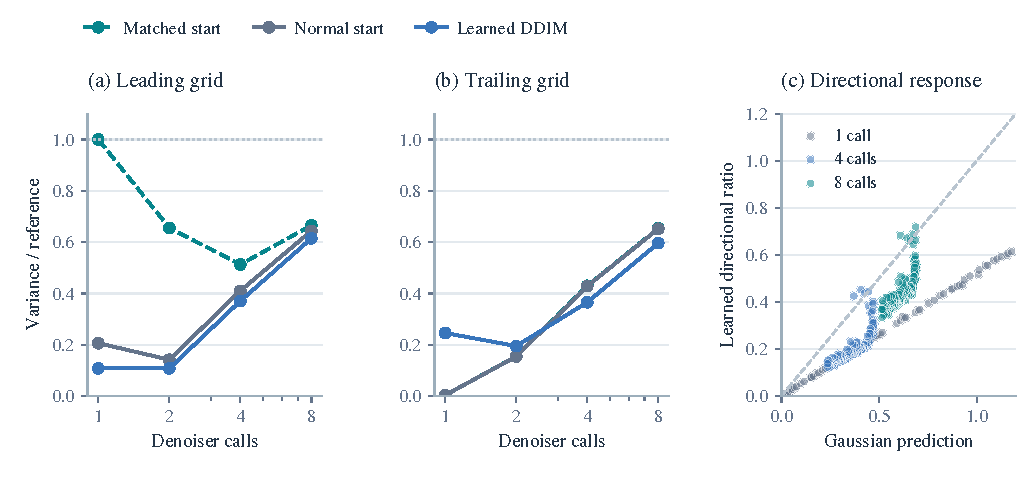
\includegraphics[width=\textwidth]{../figures/theory_initialization.pdf}
\caption{Initialization and integration in the Gaussian surrogate, with learned
CIFAR measurements in a fixed teacher-fit pixel basis. Leading spacing changes
the initial time with the budget; trailing spacing retains the noisy start.
The directional agreement at four/eight leading steps and the trailing
one-step failure delimit the empirical scope of the diagonal calculation.
These panels use the fitted reference covariance for the theory comparison;
the main benchmark metrics use independent evaluation-reference panels.}
\label{fig:cifar_theory_supp}
\end{figure*}

\begin{figure*}[t]
\centering
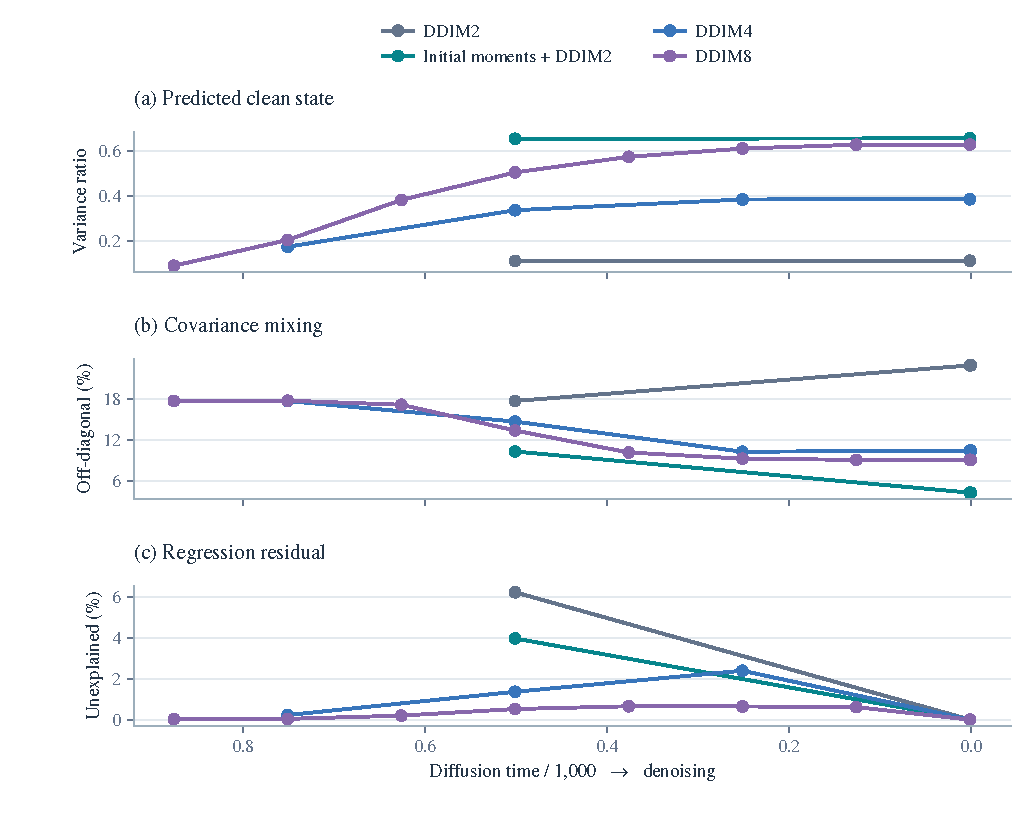
\includegraphics[width=\textwidth]{../figures/theory_trajectories.pdf}
\caption{Intermediate-state measurements in a fixed teacher-fit basis.
Estimated clean-state spread, off-diagonal covariance, and cross-step regression
residuals reveal departures from an exactly diagonal Gaussian evolution.
Projection residuals are descriptive and can include omitted-coordinate effects.}
\label{fig:cifar_trajectory_supp}
\end{figure*}

\subsection{Compute and reproducibility}
All sampling uses one H200 with float32 and at most eight CPU threads per
process. Per-arm records preserve seeds, timesteps, configuration, wall time,
peak memory, sample hashes, and source hashes. Timing reflects shared hardware
and is not a dedicated-device throughput benchmark. The complete CIFAR record
contains 403,824 images including pilot and derived-output images, and 2,256,112
denoiser-plus-JVP calls excluding reused Bures outputs and the supplied teacher.
Recorded sampling wall time totals 1,685 seconds; feature extraction and
diagnosis are additional. The primary 22-arm diagnostic takes about 60 seconds
on eight CPU threads after feature extraction, with all reference fitting
included. Frozen fits can be reused in subsequent audits.

Preparation is not free. The supplied 20,000-image DDIM100 reference represents
\textbf{2,000,000 forward-image calls}; we reuse this valid cache and do not
reconstruct its original generation wall time. The primary 22-arm pilot contains
45,056 images (22$\times$2,048), including two derived Bures outputs, and
174,080 additional denoiser calls. Its recorded generation time is 58.6 seconds;
DINO and Inception extraction records add 89.8 and 91.4 seconds. The broader
26-arm development record in Table~\ref{tab:cifar_resources} also includes four
earlier unmatched-grid solver arms.

The frozen audit's decision uses the reference-based initialization penalty at
two calls and leading-DDIM, DPM++, and UniPC pilot measurements at four/eight
calls. Those six metric inputs comprise 12,288 images and 73,728 denoiser calls;
including the two-call default and selected-remedy validation gives 16,384
images and 81,920 calls. These are input requirements of the frozen rule,
not realized savings: development actually evaluated the complete pilot.
Covariance-fit and per-image transformation wall times were not separately
recorded. ``No extra denoiser calls'' for the initializer refers only to
online sampling after preparation, not to free reference construction,
feature computation, or matrix operations. Original cached teacher-DINO
extraction time is likewise unavailable; its recorded reuse time is not
represented as extraction throughput.

The reproduction guide lists exact commands for feature extraction, generation,
metrics, diagnostics, plots, and independent confirmation. Raw outputs remain
immutable; the manifest verifies their hashes against generation records.
Editable PDF/SVG figures are generated from saved result files.
Figure~\ref{fig:initializer_examples} uses indices 7, 2007, 4007, 6007,
and 8007 in both two-call arms, with no metric-based image selection. All configurations, complete
per-panel metric arrays, gate sensitivity values, and paired contrasts are
included in the accompanying package.

% BEGIN AUTO TIMING
\begin{table*}[t]
\centering
\small
\setlength{\tabcolsep}{3.5pt}
\caption{Generation resources for every CIFAR study. Image totals include derived Bures outputs; call counts exclude their reused sampling. The supplied 20,000-image teacher and feature/metric computation are excluded. Wall time is the sum of recorded arm times on shared hardware.}
\label{tab:cifar_resources}
\begin{tabular}{lrrrr}
\toprule
Study & Arms & Images & Forward+JVP calls & Seconds \\
\midrule
Development pilot & 26 & 53,248 & 223,232 & 67.2 \\
Primary final & 22 & 220,000 & 850,000 & 333.7 \\
CAS pilot & 2 & 4,096 & 20,480 & 76.2 \\
CAS final & 2 & 20,000 & 100,000 & 328.0 \\
CAS clip adapter & 2 & 4,096 & 20,480 & 36.8 \\
Initializer ablation & 2 & 20,000 & 40,000 & 47.8 \\
Fresh initializer confirmation & 6 & 60,000 & 120,000 & 43.5 \\
Reference stability & 3 & 6,000 & 800,000 & 682.5 \\
Trajectories & 8 & 16,384 & 81,920 & 69.3 \\
\bottomrule
\end{tabular}
\end{table*}
% END AUTO TIMING


\section{Additional CIFAR models, training controls, and semantic checks}
\label{sec:supp_additional_cifar}

These completed studies test which conclusions survive a stronger pretrained
model, matched training controls, and a second classifier representation.
They complement the five-panel DDPM confirmation in the main paper; their KID, coverage, and regional-mass results are
\emph{descriptive development measurements}, with one noise panel per arm.
All declared arms are reported below. The additional studies reuse the
10,000-image CIFAR test reference. Only completed study arms contribute to these tables.

\subsection{Cost-matched solver comparisons on EDM}
We use the official unconditional CIFAR-10 VP checkpoint from
EDM~\cite{karras2022edm}, independently pretrained from the public DDPM.
The official implementation is pinned to commit
\texttt{008a4e5316c8e3bfe61a\allowbreak{}62f874bddba254295afb}; checkpoint and source
hashes are retained with the protocol. Sampling uses the power-law noise
grid with $\rho=7$, $\sigma_{\min}=0.002$, $\sigma_{\max}=80$, and
zero stochastic churn. Integration is in FP64 and the network is in FP32,
as in the official implementation. The official conversion to uint8 is
$\operatorname{clip}(127.5x+128,0,255)$, followed by integer conversion.

Euler requires one denoiser call per step. Heun requires two except at the
final step, so $K$ Heun steps require $2K-1$ calls. The complete comparison
pairs Euler at 3/7/15/35 steps with Heun at 2/4/8/18 steps.
This matches denoiser calls while allowing their integration grids to differ;
it does not isolate formal order on an identical grid. All eight arms use
2,048 paired per-image seeds beginning at 97,000,000, batch size 64, and
no result-dependent choice of seeds. Instrumented call counts and a
same-input comparison against the official Heun sampler verify the adapter:
uint8 outputs agree exactly, and floating outputs differ by at most
$10^{-10}$ under the declared check. Total generation is 16,384 images and
245,760 forward-image calls.

Table~\ref{tab:additional_edm} reports all outcomes.
At 15 calls, Heun lowers KID by 71.4\%, but its coverage and precision
are lower. At 35 calls, Heun lowers KID by 83.5\% with essentially unchanged
coverage, while its accepted-class mass error is higher. At three and
seven calls the KID ordering reverses. The joint pattern is informative:
higher integration order helps only when enough integration intervals
remain, and a better distributional quality metric need not improve every
coverage or regional statistic. High DINO precision on the three-call
Euler output is particularly misleading when considered alone: its
classifier acceptance is 1.37\%, recall is 0.026, and coverage is 0.111.
Figure~\ref{fig:edm_fixed_examples} shows the first two paired noise indices
for every arm, without ranking or replacement.

% BEGIN AUTO EDM
\begin{table*}[t]
\centering\small
\setlength{\tabcolsep}{4pt}
\caption{Complete EDM comparison. Each arm uses the same 2,048 noise seeds. Calls count denoiser evaluations; Heun uses $2K-1$ calls for $K$ steps. KID is multiplied by $10^3$; P/C/R/D are fixed-real DINO precision, coverage, recall, and density ($k=5$). MAD is the mean absolute error of ten unconditional accepted-region masses; Acc. is classifier acceptance. These are descriptive development points. Seconds are observed generation time, excluding feature extraction, on a shared H200; call counts are the controlled cost.}
\label{tab:additional_edm}
\begin{tabular}{lrrrrrrrrr}
\toprule
Sampler & Calls & KID$\downarrow$ & P & C & R & D & MAD$\downarrow$ & Acc. & Sec. \\
\midrule
Euler 3 & 3 & 202.607 & 0.868 & 0.111 & 0.026 & 3.229 & 0.0894 & 0.0137 & 14.9 \\
Heun 2 & 3 & 649.138 & 0.000 & 0.000 & 0.000 & 0.000 & 0.0907 & 0.0000 & 14.6 \\
Euler 7 & 7 & 36.549 & 0.881 & 0.341 & 0.409 & 2.320 & 0.0376 & 0.6284 & 34.1 \\
Heun 4 & 7 & 98.298 & 0.906 & 0.191 & 0.135 & 5.023 & 0.0705 & 0.3379 & 33.9 \\
Euler 15 & 15 & 8.758 & 0.856 & 0.477 & 0.638 & 1.423 & 0.0142 & 0.8418 & 73.0 \\
Heun 8 & 15 & 2.504 & 0.787 & 0.417 & 0.692 & 1.006 & 0.0118 & 0.8311 & 72.6 \\
Euler 35 & 35 & 2.500 & 0.821 & 0.501 & 0.716 & 1.136 & 0.0070 & 0.8862 & 170.3 \\
Heun 18 & 35 & 0.413 & 0.799 & 0.501 & 0.741 & 1.053 & 0.0103 & 0.8872 & 169.2 \\
\bottomrule
\end{tabular}
\end{table*}
% END AUTO EDM

\begin{figure*}[t]
\centering
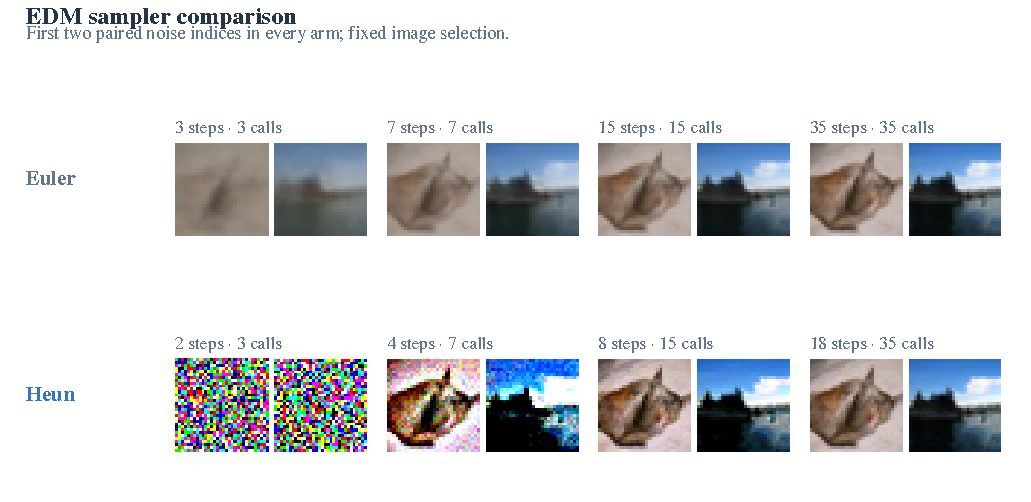
\includegraphics[width=\textwidth]{../figures/edm_quality_examples.pdf}
\caption{All eight EDM arms, using the first two fixed paired noise indices.
They are the first two indices of the prespecified first-12 example set,
with no ranking or replacement. Matching
calls changes the number of Euler versus Heun integration intervals; the
three- and seven-call failures are retained alongside the higher-budget
outputs. Quantitative conclusions use all 2,048 images per arm.}
\label{fig:edm_fixed_examples}
\end{figure*}

\paragraph{Image-frequency cross-check.}
An additional completed check measures the mean squared magnitude of the
unnormalized grayscale $32\times32$ Fourier transform outside centered
radius eight. The range is fixed from 10,000 real training images:
the 1--99\% quantile band is $[2.53593,41.11845]$, and the declared
5--95\% sensitivity band is $[4.37764,30.74381]$ (linear quantiles).
The check was motivated by visible artifacts in development images;
it is an artifact proxy, rather than a universal visual-quality definition.
It can reject legitimate unusually smooth or textured images.
The complete record covers all 58 available cached arms; the EDM arms
and relevant DDPM reference/initializer controls are shown in
Table~\ref{tab:additional_frequency}. The archived frequency display retains marginal precision and primary-band
rates with pointwise 95\% Clopper--Pearson intervals, conditional on the fixed
band. They are separate from simultaneous fidelity certification.

At seven calls, Heun's DINO precision is 0.906 but its frequency-range
rate is only 0.247. At 35 calls, Heun's frequency-range rate rises to
0.978 despite lower DINO precision. The DDPM covariance initializer also
improves the frequency-range rate from 0.0072 to 0.2470, while leaving a
substantial gap to DDIM200's 0.9720. Thus its replicated KID improvement
and coverage gain repair part of the low-budget failure; they do not
establish complete real-data fidelity. The narrower-band results and
conjunction with the fixed DINO precision event remain visible below.

% BEGIN AUTO ARTIFACT
\begin{table*}[t]
\centering\small
\setlength{\tabcolsep}{4pt}
\caption{Frequency-range cross-check: all eight EDM arms and DDPM initializer/reference controls. P is the same fixed-real DINO precision event used in each completed record. F$_{98}$ and F$_{90}$ are the fractions within the 1--99\% and 5--95\% real-training frequency ranges; P$\cap$F is their measured conjunction, not a product of marginal rates. Rows are descriptive, with no simultaneous quality certification.}
\label{tab:additional_frequency}
\begin{tabular}{lrrrrrr}
\toprule
Arm & $n$ & P & F$_{98}$ & P$\cap$F$_{98}$ & F$_{90}$ & P$\cap$F$_{90}$ \\
\midrule
Euler 3 & 2,048 & 0.8682 & 0.0137 & 0.0132 & 0.0010 & 0.0010 \\
Heun 2 & 2,048 & 0.0000 & 0.0000 & 0.0000 & 0.0000 & 0.0000 \\
Euler 7 & 2,048 & 0.8813 & 0.4492 & 0.3950 & 0.1860 & 0.1621 \\
Heun 4 & 2,048 & 0.9058 & 0.2466 & 0.2212 & 0.0776 & 0.0718 \\
Euler 15 & 2,048 & 0.8560 & 0.8853 & 0.7563 & 0.6772 & 0.5854 \\
Heun 8 & 2,048 & 0.7871 & 0.9058 & 0.7163 & 0.7427 & 0.5845 \\
Euler 35 & 2,048 & 0.8213 & 0.9629 & 0.7905 & 0.8730 & 0.7197 \\
Heun 18 & 2,048 & 0.7988 & 0.9780 & 0.7827 & 0.8940 & 0.7197 \\
DDPM leading2 & 10,000 & 0.9410 & 0.0072 & 0.0067 & 0.0005 & 0.0005 \\
DDPM initial covariance2 & 10,000 & 0.9544 & 0.2470 & 0.2348 & 0.1003 & 0.0947 \\
DDPM DDIM200 & 2,000 & 0.7890 & 0.9720 & 0.7650 & 0.9000 & 0.7065 \\
\bottomrule
\end{tabular}
\end{table*}
% END AUTO ARTIFACT

\subsection{Matched natural-image training controls}
\paragraph{Training and pairing.}
All three adapted states start from the same public
\texttt{google/ddpm-cifar10-32} checkpoint, pinned to revision
\texttt{267b167dc01f0e4e6192\allowbreak{}3ea244e8b988f84deb80}.
They receive 3,000 updates with one shared adaptation seed, 85,001,
batch size 128, learning rate $2\times10^{-5}$, dropout 0.1, and a new
Adam state because the public checkpoint contains no optimizer state.
Adam uses $(\beta_1,\beta_2)=(0.9,0.999)$, $\epsilon=10^{-8}$, and
zero weight decay. We clip the gradient norm to one and maintain an EMA
with decay 0.999, initialized from the public weights.
The objective is epsilon-prediction MSE with a uniformly sampled timestep:
$x_t=\sqrt{\bar\alpha_t}x_0+\sqrt{1-\bar\alpha_t}\epsilon$.
There are 1,000 training noise levels with linear betas from $10^{-4}$ to
0.02. Images are mapped to $[-1,1]$ and flipped horizontally with
probability 0.5. Forward computation uses BF16; model masters, loss,
Adam state, and EMA use FP32, with TF32 disabled and deterministic
algorithms enabled.

The controls change only the distribution used to draw labeled training
examples. \emph{Uniform} samples all ten classes equally.
\emph{Cat $3\times$} repeats each cat example three times, so cats have
25\% of the resulting 60,000-example mixture.
\emph{Ratio} uses all ten classifier-event residuals from an earlier,
disjoint 2,000-image public DPM++25 pilot. Let $p_j$ and $q_j$ denote the
unconditional accepted-region frequencies in the real reference and that
pilot, and let $p_R,q_R$ be rejection frequencies. The heuristic sets
weights $w_j$ by clipping the accepted-only frequency ratio to $[0.5,2]$
and normalizes them over the ten classes indexed by $k$:
\begin{equation}
\begin{aligned}
 w_j&=\operatorname{clip}\!\left(
 \frac{p_j/(1-p_R)}{q_j/(1-q_R)},\;0.5,\;2\right),\\
 \Pr(\text{training class}=j)&=\frac{w_j}{\sum_k w_k}.
\end{aligned}
\label{eq:supp_class_weighting}
\end{equation}
The class probabilities in label order, rounded here to four decimals, are
0.1239, 0.0835, 0.1289, 0.0670, 0.1120, 0.1019, 0.0528, 0.0958,
0.1407, and 0.0934. Exact values are frozen in the training protocol.
The ratio is an intervention hypothesis, not an inverse model of how
training frequencies determine generated frequencies.

Uniform and Ratio consume the same uniform random draws through their
inverse sampling CDFs. A saved check verifies matching RNG consumption
against the existing cat branch, including subsequent flips, noise,
timesteps, and dropout. Checkpoints every 500 updates retain model, EMA,
optimizer, RNG states, and hashes; full per-update histories are preserved.
A five-update interrupted/resumed segment reproduces model, EMA, Adam,
RNG state, and losses exactly. This pairing controls optimization noise
within the study; one adaptation seed does not quantify across-training
variability, and all branches share one pretrained base.

\paragraph{Complete evaluation.}
The unmodified public state and all three adapted states are evaluated
with DDIM25, DDIM50, and DPM++25. A separately declared extension evaluates
DPM++8 and UniPC8 on the same four states. All use trailing timesteps,
2,000 paired fresh seeds 98,000,000--98,001,999, FP32 sampling, batch 128,
and the same frozen classifiers and feature extractors. Generation totals
40,000 images and 928,000 forward-image calls; the two newly trained
controls add 6,000 optimizer updates. Table~\ref{tab:additional_training}
retains all 20 arms. The main text's public DPM++25 control is regenerated
on this fresh panel; the older pilot is used only to define the Ratio
weights and the separate reference-sensitivity check.

The regional error is
$\operatorname{MAD}_{10}=\frac{1}{10}\sum_{j=0}^9|q_j-p_j|$,
with all samples, including rejected images, in each denominator.
Thus a high rejection rate cannot disappear through renormalization.
KID is the unbiased cubic-kernel MMD in Inception features against the
fixed 10,000-image real reference. DINO precision uses membership in the
union of those real images' fifth-neighbor balls; coverage is the fraction
of real balls reached by any generated point. Recall uses generated
fifth-neighbor balls, and density averages the number of real balls
containing each generated point, divided by five.
These are the exact fixed-real events used in the reported quality gates;
values from a differently subsampled PRDC reference are not substituted.

Table~\ref{tab:additional_training_contrasts} preserves every declared
same-sampler comparison. For classifier acceptance and fixed-real DINO
precision, the paired-Bernoulli interval in the methods supplement bounds
the candidate-minus-reference probability difference using four
Clopper--Pearson tails per comparison. We use $\alpha=0.05$, a
five-percentage-point noninferiority margin, and families of 36 and 24
binary comparisons for the long-step and eight-call studies, respectively.
All statements condition on the frozen trained checkpoints, classifiers,
and fixed real geometry. They do not quantify uncertainty over training
seeds. A joint pass requires both event lower bounds to exceed $-0.05$;
otherwise the result can remain inconclusive.

Uniform continuation improves KID and mass error over the public state
under every sampler. The Ratio intervention has worse KID under all five
samplers and worse mass error under the three long-step probes than
Uniform; at eight calls it slightly improves mass error while losing KID
and coverage. Cat oversampling also has worse KID and mass error than
Uniform, and its quality noninferiority relative to Uniform remains
inconclusive under every sampler. These controls show why an observed
class-region residual alone is insufficient to prescribe class reweighting.

% BEGIN AUTO TRAINING
\begin{table*}[t]
\centering\small
\setlength{\tabcolsep}{4pt}
\caption{Complete natural-image training-control study: four states and five samplers, with 2,000 paired fresh noise seeds per arm. Uniform, Ratio, and Cat $3\times$ each receive 3,000 updates from the same public base and one adaptation seed. All point estimates condition on those trained states and the reused real reference; they are not independent-training-seed estimates. P/C/R/D and Acc. have the definitions of Table~\ref{tab:additional_edm}; Cat err. is the absolute error of the unconditional accepted cat-region mass.}
\label{tab:additional_training}
\begin{tabular}{llrrrrrrrr}
\toprule
Sampler & Training & KID$\times10^3\downarrow$ & P & C & R & D & MAD$\downarrow$ & Cat err.$\downarrow$ & Acc. \\
\midrule
DDIM25 & Public & 18.253 & 0.780 & 0.315 & 0.543 & 1.286 & 0.0307 & 0.0218 & 0.7210 \\
DDIM25 & Uniform & 13.307 & 0.791 & 0.350 & 0.578 & 1.136 & 0.0165 & 0.0043 & 0.7515 \\
DDIM25 & Ratio & 13.617 & 0.785 & 0.344 & 0.589 & 1.123 & 0.0178 & 0.0122 & 0.7540 \\
DDIM25 & Cat $3\times$ & 16.382 & 0.795 & 0.347 & 0.585 & 1.351 & 0.0260 & 0.0458 & 0.7395 \\
\midrule
DDIM50 & Public & 13.493 & 0.784 & 0.328 & 0.585 & 1.286 & 0.0248 & 0.0048 & 0.7470 \\
DDIM50 & Uniform & 9.589 & 0.787 & 0.356 & 0.627 & 1.128 & 0.0143 & 0.0047 & 0.7645 \\
DDIM50 & Ratio & 10.051 & 0.784 & 0.349 & 0.626 & 1.090 & 0.0170 & 0.0217 & 0.7770 \\
DDIM50 & Cat $3\times$ & 12.228 & 0.793 & 0.347 & 0.622 & 1.287 & 0.0233 & 0.0343 & 0.7430 \\
\midrule
DPM++25 & Public & 14.786 & 0.752 & 0.308 & 0.600 & 0.996 & 0.0247 & 0.0018 & 0.7375 \\
DPM++25 & Uniform & 10.096 & 0.766 & 0.338 & 0.637 & 0.949 & 0.0148 & 0.0092 & 0.7595 \\
DPM++25 & Ratio & 10.899 & 0.757 & 0.334 & 0.639 & 0.912 & 0.0176 & 0.0212 & 0.7735 \\
DPM++25 & Cat $3\times$ & 12.477 & 0.763 & 0.336 & 0.626 & 1.041 & 0.0242 & 0.0353 & 0.7360 \\
\midrule
DPM++8 & Public & 26.943 & 0.794 & 0.306 & 0.437 & 1.516 & 0.0369 & 0.0558 & 0.6500 \\
DPM++8 & Uniform & 21.767 & 0.805 & 0.336 & 0.490 & 1.281 & 0.0255 & 0.0243 & 0.7010 \\
DPM++8 & Ratio & 22.333 & 0.798 & 0.333 & 0.491 & 1.259 & 0.0242 & 0.0083 & 0.7045 \\
DPM++8 & Cat $3\times$ & 25.118 & 0.799 & 0.328 & 0.495 & 1.435 & 0.0378 & 0.0743 & 0.6785 \\
\midrule
UniPC8 & Public & 25.240 & 0.792 & 0.303 & 0.445 & 1.333 & 0.0359 & 0.0553 & 0.6630 \\
UniPC8 & Uniform & 19.527 & 0.786 & 0.340 & 0.507 & 1.176 & 0.0239 & 0.0263 & 0.7210 \\
UniPC8 & Ratio & 20.391 & 0.780 & 0.334 & 0.505 & 1.142 & 0.0227 & 0.0048 & 0.7135 \\
UniPC8 & Cat $3\times$ & 22.988 & 0.796 & 0.334 & 0.505 & 1.322 & 0.0347 & 0.0673 & 0.6955 \\
\bottomrule
\end{tabular}
\end{table*}
% END AUTO TRAINING

% BEGIN AUTO CONTRASTS
\begin{table*}[t]
\centering\small
\setlength{\tabcolsep}{4pt}
\caption{All 30 declared same-sampler training contrasts. Negative KID and MAD differences favor the first state. Intervals bound the candidate-minus-reference acceptance (Acc.) and fixed-real DINO precision (P) differences. The exact paired-Bernoulli construction controls a 36-event family for the three long-step samplers and a separate 24-event family for the two eight-call samplers; the two families are not jointly a single 95\% statement. Pass requires both lower bounds to exceed $-0.05$. Inconclusive is not a demonstrated quality loss; passing permits losses within the stated margin. Decisions use unrounded bounds; KID/MAD differences are descriptive.}
\label{tab:additional_training_contrasts}
\begin{tabular}{llrrlll}
\toprule
Sampler & Contrast & $\Delta$KID$\times10^3$ & $\Delta$MAD & $\Delta$Acc. interval & $\Delta$P interval & Joint NI \\
\midrule
DDIM25 & Uniform $-$ Public & -4.946 & -0.0143 & [-0.0110, +0.0788] & [-0.0298, +0.0545] & Pass \\
DDIM25 & Ratio $-$ Public & -4.636 & -0.0129 & [-0.0090, +0.0821] & [-0.0382, +0.0494] & Pass \\
DDIM25 & Cat $3\times$ $-$ Public & -1.871 & -0.0048 & [-0.0225, +0.0638] & [-0.0251, +0.0588] & Pass \\
DDIM25 & Ratio $-$ Uniform & +0.310 & +0.0014 & [-0.0330, +0.0388] & [-0.0422, +0.0283] & Pass \\
DDIM25 & Cat $3\times$ $-$ Uniform & +3.075 & +0.0095 & [-0.0502, +0.0226] & [-0.0302, +0.0395] & Inconcl. \\
DDIM25 & Ratio $-$ Cat $3\times$ & -2.765 & -0.0082 & [-0.0237, +0.0565] & [-0.0494, +0.0265] & Pass \\
DDIM50 & Uniform $-$ Public & -3.904 & -0.0105 & [-0.0236, +0.0627] & [-0.0389, +0.0445] & Pass \\
DDIM50 & Ratio $-$ Public & -3.442 & -0.0077 & [-0.0110, +0.0778] & [-0.0439, +0.0428] & Pass \\
DDIM50 & Cat $3\times$ $-$ Public & -1.265 & -0.0014 & [-0.0481, +0.0391] & [-0.0302, +0.0506] & Pass \\
DDIM50 & Ratio $-$ Uniform & +0.463 & +0.0028 & [-0.0192, +0.0484] & [-0.0383, +0.0313] & Pass \\
DDIM50 & Cat $3\times$ $-$ Uniform & +2.640 & +0.0090 & [-0.0603, +0.0106] & [-0.0270, +0.0421] & Inconcl. \\
DDIM50 & Ratio $-$ Cat $3\times$ & -2.177 & -0.0063 & [+0.0002, +0.0771] & [-0.0484, +0.0267] & Pass \\
DPM++25 & Uniform $-$ Public & -4.690 & -0.0099 & [-0.0199, +0.0689] & [-0.0286, +0.0598] & Pass \\
DPM++25 & Ratio $-$ Public & -3.886 & -0.0071 & [-0.0053, +0.0852] & [-0.0398, +0.0498] & Pass \\
DPM++25 & Cat $3\times$ $-$ Public & -2.309 & -0.0005 & [-0.0461, +0.0427] & [-0.0321, +0.0555] & Pass \\
DPM++25 & Ratio $-$ Uniform & +0.803 & +0.0028 & [-0.0179, +0.0505] & [-0.0475, +0.0256] & Pass \\
DPM++25 & Cat $3\times$ $-$ Uniform & +2.381 & +0.0094 & [-0.0634, +0.0093] & [-0.0413, +0.0333] & Inconcl. \\
DPM++25 & Ratio $-$ Cat $3\times$ & -1.577 & -0.0066 & [+0.0030, +0.0812] & [-0.0468, +0.0332] & Pass \\
DPM++8 & Uniform $-$ Public & -5.176 & -0.0114 & [+0.0099, +0.1001] & [-0.0273, +0.0520] & Pass \\
DPM++8 & Ratio $-$ Public & -4.610 & -0.0127 & [+0.0110, +0.1058] & [-0.0379, +0.0457] & Pass \\
DPM++8 & Cat $3\times$ $-$ Public & -1.825 & +0.0008 & [-0.0120, +0.0750] & [-0.0341, +0.0453] & Pass \\
DPM++8 & Ratio $-$ Uniform & +0.566 & -0.0013 & [-0.0306, +0.0387] & [-0.0419, +0.0245] & Pass \\
DPM++8 & Cat $3\times$ $-$ Uniform & +3.351 & +0.0123 & [-0.0617, +0.0103] & [-0.0393, +0.0253] & Inconcl. \\
DPM++8 & Ratio $-$ Cat $3\times$ & -2.784 & -0.0135 & [-0.0099, +0.0684] & [-0.0377, +0.0342] & Pass \\
UniPC8 & Uniform $-$ Public & -5.713 & -0.0119 & [+0.0161, +0.1077] & [-0.0483, +0.0338] & Pass \\
UniPC8 & Ratio $-$ Public & -4.849 & -0.0131 & [+0.0082, +0.1007] & [-0.0559, +0.0281] & Inconcl. \\
UniPC8 & Cat $3\times$ $-$ Public & -2.252 & -0.0012 & [-0.0079, +0.0797] & [-0.0356, +0.0446] & Pass \\
UniPC8 & Ratio $-$ Uniform & +0.864 & -0.0012 & [-0.0433, +0.0261] & [-0.0401, +0.0262] & Pass \\
UniPC8 & Cat $3\times$ $-$ Uniform & +3.461 & +0.0107 & [-0.0641, +0.0056] & [-0.0211, +0.0455] & Inconcl. \\
UniPC8 & Ratio $-$ Cat $3\times$ & -2.597 & -0.0119 & [-0.0189, +0.0595] & [-0.0549, +0.0172] & Inconcl. \\
\bottomrule
\end{tabular}
\end{table*}
% END AUTO CONTRASTS

\subsection{Calibrated classifier regions and reference robustness}
\paragraph{Two-classifier consensus.}
Two CIFAR-stem ResNet-18 classifiers are trained from scratch with seeds
84,001 and 84,002. A single unstratified permutation with seed 84,000
splits the 50,000 training images into 45,000 fitting, 2,500 temperature,
and 2,500 acceptance-calibration images. Both use the fixed final
checkpoint at epoch 200. Training uses batch 256, SGD with learning rate
0.1, momentum 0.9, Nesterov updates, weight decay $5\times10^{-4}$,
five warmup epochs followed by cosine decay, reflect-padding by four
pixels, random $32\times32$ cropping, and horizontal flips.
There is no label smoothing or validation-based checkpoint selection.

Separate temperature fits minimize held-out NLL, giving temperatures
1.29126 and 1.27755. An image is accepted only when both classifiers
predict the same class and both calibrated maximum probabilities exceed
a common threshold. Before training, we declare the 14 thresholds
$\{.5,.6,.7,.75,.8,.85,.9,.92,.94,.96,.97,.98,.99,.995\}$.
The lowest eligible threshold must accept at least 500 calibration images
and have a one-sided Clopper--Pearson selective-error upper bound at most
0.02, using tail probability $0.05/14$ to account for threshold selection.
The selected threshold is 0.8: 24 errors among 2,310 accepted calibration
images yield an upper bound of 0.01748. Only then is the official test set
used for reporting. Individual test accuracies are 95.32\% and 95.30\%;
consensus accepts 9,075/10,000 images with 98.7548\% accuracy among them.
Class-region masses are compared with these measured real accepted-region
masses, rather than the nominal 0.1 label proportions.

The guarantee concerns real validation inputs under the sampling
assumption. It does not establish generated-image semantic correctness.
Accordingly, we call these \emph{accepted classifier regions}, retain the
reject event, and inspect unranked examples. No human annotation or
true-label guarantee for generated samples is inferred from classifier
agreement. Primary inference uses the frozen BF16 classifier computation;
CPU/FP32 checks and any event disagreements are recorded separately.

\paragraph{Independent classifier representation.}
A second check fits a multinomial linear classifier on frozen DINOv2
features~\cite{oquab2024dinov2}. From 10,000 CIFAR training images, a
permutation with seed 87,300 assigns 8,000 to fitting, 1,000 to temperature
fitting, and 1,000 to calibration reporting. Standardization uses only
the fitting pool, with standard deviations floored at $10^{-6}$.
The classifier uses $C=1$, LBFGS, maximum 2,000 iterations, and tolerance
$10^{-8}$. Its temperature is 1.51259. The acceptance threshold 0.8 is fixed
before this fit; no threshold is selected on its test results.
On the official real test set, accuracy is 97.52\%, acceptance is 95.66\%,
and accepted accuracy is 99.09\%. The check includes all 50 previously
cached DDPM arms and all eight EDM arms. It changes the classifier
architecture, while DINO's pretrained representation also supplies the
geometric quality measurement; these are not fully independent sources
of semantic evidence.

Table~\ref{tab:additional_reference_regions} exposes why the reference
choice matters. The public DPM++25 frog-region excess decreases under
DDIM200 with either classifier. The DPM++100 comparison retains the frog-region excess. The three resolved probes share their
noise panel, while DPM++25 is from the earlier development pilot.
Together with the numerical reference-stability experiment, this makes
sampler convergence an empirical check rather than an assumption based
only on the number of steps. All displayed masses are fixed-event
observations; none establishes persistent absence or excess of true
semantic classes in the underlying learned distribution.

% BEGIN AUTO FREQUENCY
\begin{table*}[t]
\centering\small
\setlength{\tabcolsep}{4pt}
\caption{Reference sensitivity under two frozen classifiers. All masses are unconditional, retaining rejection in the denominator. Each generated probe has 2,000 images; the three 100/200-call probes share a separate noise panel from the DPM++25 development pilot. The numerical frequencies differ across classifiers, but the frog-region discrepancy shrinks under DDIM200 in both. These are descriptive fixed-event measurements, not verified generated-image class labels or a certificate of population representativeness.}
\label{tab:additional_reference_regions}
\begin{tabular}{lrrrrrr}
\toprule
Probe & CNN airplane & CNN frog & CNN reject & DINO airplane & DINO frog & DINO reject \\
\midrule
Real test & 0.0913 & 0.0943 & 0.0925 & 0.0970 & 0.0975 & 0.0434 \\
DPM++25 & 0.0570 & 0.1380 & 0.2385 & 0.0545 & 0.1380 & 0.2835 \\
DPM++100 & 0.0585 & 0.1470 & 0.2535 & 0.0580 & 0.1385 & 0.3015 \\
DDIM100 & 0.0665 & 0.1175 & 0.2490 & 0.0630 & 0.1170 & 0.3000 \\
DDIM200 & 0.0890 & 0.1030 & 0.2345 & 0.0790 & 0.1045 & 0.2825 \\
\bottomrule
\end{tabular}
\end{table*}
% END AUTO FREQUENCY

\paragraph{Reproduction and numerical provenance.}
\texttt{code/cifar\_additional\_tables.py} renders every table in this
section from the completed JSON reports. It checks report/protocol hashes,
arm counts, sample and call totals, unconditional masses, arithmetic of all
30 contrasts, and fidelity-status consistency before exporting.
The accompanying provenance JSON records exact unrounded values and source
hashes. Original sample arrays, feature arrays, generation metadata,
checkpoint receipts, and unranked first-index grids remain in the evidence
package. The complete eight-arm EDM and 20-arm training tables are
reproducible without fitting or running a GPU when those reports are
available; regenerating their images requires the pinned implementation
and checkpoints described by their protocols.

\section{Signed semantic measurements and independent repairs}
\label{supp:mnist}

\paragraph{Study structure.}
Validated semantic regions make missing mass and overcorrection separately
measurable. The original restoration study tests a withheld digit; the
separate equal-update follow-up repairs excess mass in targeted parents.
A third study crosses existing checkpoints with numerical probes. All three
retain their own diagnosis samples, outcome samples, and comparison families. The training
set is the official 60,000-image MNIST training split. We withhold every image
of digit 3 in the initial phase. The 10,000 official test images are reserved
for evaluation and measurement validation. The generator is unconditional;
its training code does not use digit labels except to construct the declared
training subsets. Digit 3 and the branch definitions are fixed before any
confirmatory training seed is initialized.

Three independent training seeds (10, 11, 12) each train for 25,000 updates on
the withheld dataset. From the same model, EMA, and optimizer checkpoint,
three equal-compute branches perform 8,000 further updates: continue on the
withheld data, restore the full training data, or restore it with digit-3
examples duplicated once. The targeted branch's duplication weight is two,
chosen in a separate seed-98 pilot. A fourth baseline trains on the full data
from initialization for 33,000 updates. All continuation branches use the
same branch RNG seed, initial state, optimizer settings, and number of updates.
The targeted branch is an explicit sensitivity to restoring more missing-class
mass; its effects on every other class remain in the evaluation.

\paragraph{Network and optimization.}
The denoiser is a \texttt{diffusers.UNet2DModel} for $28\times28$ single-channel
images, with block widths 32/64/64, two layers per block, middle-resolution
attention, and GroupNorm with eight groups. The forward diffusion has 1,000
steps and the library's linear beta schedule. Each update samples 128 training
examples with replacement and independent uniform timesteps; the objective is
mean squared epsilon-prediction error. AdamW uses learning rate $2\times10^{-4}$
and weight decay $10^{-4}$. Gradients are clipped at norm one. Model forward
passes use BF16 autocast; optimization and EMA states remain FP32. The EMA decay
at zero-indexed global update $u$ is
$\min(0.999,(1+u)/(10+u))$, avoiding a long contribution from the untrained
initialization in short runs. Checkpoints preserve the model, EMA, optimizer,
update count, configuration, and CUDA RNG state. Training-loss and runtime logs
are retained for every branch.

\paragraph{Independent semantic measurement.}
Two separately initialized convolutional classifiers use seeds 2801 and 2802.
Each has convolution widths 32/64/64, two max-pooling stages, a 128-dimensional
fully connected feature layer, and a ten-class head. For each seed, a random
50,000/10,000 split of the official training data supplies six epochs of
cross-entropy training and temperature calibration, respectively. Temperature
is optimized on the held-out validation logits; test images do not tune it.
Official test accuracies are 99.08\% and 99.09\%.

The semantic cell for digit $j$ contains images on which both classifiers
predict $j$ with probabilities at least 0.9. All other images enter an explicit
rejection cell. This same function is applied to real and generated images;
true test labels are used to validate the function, never as different regions
for the real sample. On test data, the consensus cells cover 95.46\% of images
and classify 99.916\% of accepted images correctly (eight errors among 9,546).
The digit-3 cell contains 983 test images, of which 982 have true label 3.
These are held-out real-image validation results. Generated-image fidelity is
assessed separately, and uncurated sample grids permit inspection of failures.
Rejected generated images remain in every probability denominator.

\paragraph{Sampling and representation.}
For each of five model states and each training seed, all eleven prespecified
samplers generate 5,000 images: leading DDIM at 2/4 steps; trailing DDIM at
4/8/10/25/50 steps; and trailing DPM-Solver++2M at 4/8/10/25 steps. The primary
resolved probe is DPM++25. Each image receives its own initial-noise generator
with seed $6{,}100{,}000+10{,}000s+i$ for training seed $s$ and image index $i$.
Noise is paired across all states and sampler configurations within a training
seed. Scheduler timestep arrays are saved. Images are clamped, quantized to
8-bit pixels, and only then classified and embedded, so stored pixels reproduce
the measurements. Features are the first classifier's 128-dimensional hidden
layer.

\paragraph{Statistics and quality constraints.}
Semantic occupancy uses all 10,000 reference test images and the same eleven
consensus/rejection cells. The exact certificate allocates
$\alpha_{\rm semantic}=0.025$ over $11\times165$ declared cell--arm comparisons,
with retention 0.5 and minimum reference mass 0.01. The additional generic
feature audit uses 3,000 test images for PCA/partition fitting, the next 2,000
for support calibration, and the final 5,000 for evaluation. Its occupancy and
support allocations are 0.0125 each. Semantic conditional spread is a separately
frozen secondary analysis in unwhitened reference-fit PCA32 coordinates,
using the final 5,000 reference images and at least 30 images per semantic cell.
Its log-influence intervals use nominal level $0.05/(10\times165)$ and retain
their approximate status.

Nearest-neighbor fidelity and coverage use five disjoint, paired 1,000-image
panels, with $k=5$. The primary uncertainty unit is the independent training
seed, not a generated image. We average panel metrics within each seed, then
use paired Student-$t$ intervals across the three seeds. These intervals
condition on the shared real-data reference and are approximate
under a normal paired-effect assumption with only two degrees of freedom.
The primary comparisons
are targeted restoration versus continued withholding, ordinary restoration
versus continued withholding, and targeted versus ordinary restoration.
Digit-3 occupancy contrasts use Bonferroni 98.333\% intervals for this three-test
family. Ordinary 95\% intervals for the other reported metrics are descriptive.
The ten-region mass error is the mean absolute difference from real consensus
region probabilities, without renormalizing accepted images. It exposes any
loss in other digit regions when missing-class mass increases.

The resolved full-data model supplies a learned-model fidelity baseline. A
repair passes the predeclared noninferiority criterion only if the paired
95\% lower confidence bounds for both feature precision and consensus acceptance
are at least $-0.05$ relative to this baseline. An upper bound below $-0.05$
fails the criterion; all other cases are inconclusive. With three training
seeds these intervals can remain broad. The protocol preserves that uncertainty
and reports real-data support separately.

\paragraph{Qualitative selection and exclusions.}
The independent seed-98 pilot is excluded from every reported training-seed
interval. Qualitative grids show the first twelve generation indices of seed
10 for every declared row, with no quality ranking. Complete samples,
probabilities, features, and configurations accompany the results.

\subsection{Ordinary restoration recovers the missing region}
All 15 training branches reached their frozen endpoints, and all 165
5,000-image evaluations passed metadata, count, and checksum validation before
analysis. The study performs 246,000 optimization updates (31,488,000 training
example evaluations) and samples 825,000 images using 11,250,000 denoiser-image
calls. Summed recorded training-process time is 18,565 seconds, with 1,891
additional seconds for generation, feature extraction, and saving. Three jobs
share one H200, so summed process times are not dedicated-device elapsed hours.
The checkpoint/log manifest preserves each recorded segment and hash.

The ordinary restoration result is the strongest balanced repair. At DPM++25,
its ten-region mass error is $0.00953\pm0.00254$, compared with
$0.01471\pm0.00306$ for continued withholding and $0.00849\pm0.00110$ for
full-data training. Coverage is $0.7771\pm0.0145$, compared with
$0.7274\pm0.0177$ and $0.7881\pm0.0122$, respectively. Ordinary restoration
has precision $0.7407\pm0.0123$, a paired loss of 0.01407
[0.01076,0.01737] versus continued withholding. Relative to the full-data
baseline, its precision difference is $-0.01013$ [$-0.02131,0.00105$]
and consensus-acceptance difference is $-0.00933$ [$-0.02502,0.00635$].
Both meet the declared $-0.05$ lower-bound criterion. The same conjunction
passes for DDIM25 and DDIM50. These are the predeclared per-comparison
constraints, not a simultaneous all-sampler noninferiority statement.

Targeted restoration is a material counterexample to maximizing missing-region
mass. Its digit-3 mass is 0.1618, compared with the real reference's 0.0983,
and its ten-region error rises to $0.02150\pm0.00349$. Its coverage
($0.7761\pm0.0128$) is similar to ordinary restoration. The complete primary
contrasts preserve both its larger digit-3 gain and its worse overall class-mass
balance. Reject probabilities remain in every denominator.

The secondary semantic-spread control also detects crossing mechanisms.
At leading DDIM2, withheld models exhibit conditional contraction in eight
eligible digit cells in every seed, together with persistent digit-3 depletion;
two cells per seed lack sufficient samples. At DPM++25, those eight
contractions are no longer flagged, but the depleted digit remains ineligible
for spread. Full-data leading-DDIM2 models show eight or nine contractions,
whereas their DPM++25 outputs show no contraction (one seed has one expansion).
These approximate, fixed-family measurements motivate a mixed interpretation;
an ineligible cell does not establish absence of contraction.

\begin{table*}[t]
\centering\footnotesize
\setlength{\tabcolsep}{3.5pt}
\caption{All three prespecified paired effects at DPM++25, in percentage points. Digit-3 consensus-region mass uses Bonferroni 98.333\% intervals for this three-test family; mass error and feature coverage use descriptive 95\% intervals. Lower class-mass error is better. Intervals are approximate Student-$t$ intervals over three training seeds, conditional on the fixed real reference.}
\label{tab:mnist_primary_contrasts}
\begin{tabular}{lccc}
\toprule
Paired contrast & $\Delta$ digit-3 mass & $\Delta$ class-mass error & $\Delta$ coverage \\
\midrule
Targeted $-$ Continue & $16.09\,[14.02,18.17]$ & $0.68\,[0.04,1.32]$ & $4.87\,[4.05,5.70]$ \\
Restore $-$ Continue & $8.66\,[7.68,9.64]$ & $-0.52\,[-0.91,-0.12]$ & $4.97\,[4.42,5.51]$ \\
Targeted $-$ Restore & $7.43\,[4.50,10.37]$ & $1.20\,[0.84,1.55]$ & $-0.09\,[-1.07,0.88]$ \\
\bottomrule
\end{tabular}
\end{table*}

\begin{table*}[t]
\centering\footnotesize
\setlength{\tabcolsep}{3.5pt}
\caption{Resolved-sampler fidelity relative to the full-data DPM++25 model. Differences and paired 95\% intervals are in percentage points. A pass requires both lower bounds to exceed $-5$; an upper bound below $-5$ fails, and other cases are inconclusive. These are separate per-comparison conjunctions, not an all-phase simultaneous guarantee.}
\label{tab:mnist_quality}
\begin{tabular}{lccc}
\toprule
Phase & $\Delta$ precision & $\Delta$ acceptance & Joint gate \\
\midrule
Initial withheld (25k) & $-0.70\,[-1.42,0.02]$ & $-0.43\,[-1.70,0.84]$ & Pass \\
Continue withheld (33k) & $0.39\,[-1.01,1.80]$ & $0.25\,[-0.64,1.15]$ & Pass \\
Restore data (33k) & $-1.01\,[-2.13,0.10]$ & $-0.93\,[-2.50,0.63]$ & Pass \\
Targeted restoration (33k) & $-0.45\,[-1.46,0.57]$ & $-0.49\,[-1.48,0.51]$ & Pass \\
\bottomrule
\end{tabular}
\end{table*}

\begin{table*}[t]
\centering\footnotesize
\setlength{\tabcolsep}{3.5pt}
\caption{Initial withheld (25k): all eleven frozen samplers. All entries are percentages, reported as mean $\pm$ the approximate 95\% interval half-width over three training seeds. MAD is the mean absolute difference across the ten unconditional semantic-region probabilities. The final column compares precision and acceptance with the full-data model at the same sampler, using the frozen five-percentage-point noninferiority margin. These all-arm intervals are descriptive.}
\label{tab:mnist_all_withheld}
\begin{tabular}{lcccccc}
\toprule
Sampler & Digit-3 mass & MAD$\downarrow$ & Precision & Coverage & Acceptance & Fidelity \\
\midrule
Leading DDIM 2 & $0.07\pm0.03$ & $6.14\pm0.65$ & $68.56\pm1.00$ & $10.63\pm2.80$ & $34.04\pm6.46$ & Pass \\
Leading DDIM 4 & $0.21\pm0.03$ & $2.82\pm0.13$ & $74.09\pm0.36$ & $61.09\pm4.16$ & $68.83\pm2.71$ & Pass \\
Trailing DDIM 4 & $0.19\pm0.08$ & $2.72\pm0.10$ & $75.11\pm1.07$ & $60.95\pm4.30$ & $68.71\pm2.19$ & Pass \\
Trailing DDIM 8 & $0.19\pm0.10$ & $1.71\pm0.17$ & $74.03\pm1.37$ & $70.09\pm1.17$ & $80.11\pm3.07$ & Pass \\
Trailing DDIM 10 & $0.17\pm0.13$ & $1.60\pm0.14$ & $74.24\pm1.00$ & $70.95\pm1.99$ & $81.75\pm2.88$ & Pass \\
Trailing DDIM 25 & $0.09\pm0.14$ & $1.51\pm0.33$ & $74.39\pm0.63$ & $71.95\pm1.63$ & $85.29\pm2.39$ & Pass \\
Trailing DDIM 50 & $0.09\pm0.14$ & $1.50\pm0.33$ & $74.15\pm0.98$ & $72.02\pm1.86$ & $86.19\pm2.18$ & Pass \\
DPM++ 4 & $0.15\pm0.08$ & $2.33\pm0.09$ & $74.99\pm0.38$ & $66.36\pm3.29$ & $72.75\pm3.35$ & Pass \\
DPM++ 8 & $0.17\pm0.08$ & $1.51\pm0.25$ & $74.00\pm1.17$ & $72.28\pm1.66$ & $83.70\pm3.02$ & Pass \\
DPM++ 10 & $0.13\pm0.08$ & $1.52\pm0.28$ & $74.26\pm1.35$ & $72.06\pm2.13$ & $84.85\pm2.39$ & Pass \\
DPM++ 25 & $0.10\pm0.13$ & $1.49\pm0.38$ & $74.39\pm0.51$ & $72.04\pm1.69$ & $86.71\pm1.99$ & Pass \\
\bottomrule
\end{tabular}
\end{table*}

\begin{table*}[t]
\centering\footnotesize
\setlength{\tabcolsep}{3.5pt}
\caption{Continue withheld (33k): all eleven frozen samplers. All entries are percentages, reported as mean $\pm$ the approximate 95\% interval half-width over three training seeds. MAD is the mean absolute difference across the ten unconditional semantic-region probabilities. The final column compares precision and acceptance with the full-data model at the same sampler, using the frozen five-percentage-point noninferiority margin. These all-arm intervals are descriptive.}
\label{tab:mnist_all_continue_withheld}
\begin{tabular}{lcccccc}
\toprule
Sampler & Digit-3 mass & MAD$\downarrow$ & Precision & Coverage & Acceptance & Fidelity \\
\midrule
Leading DDIM 2 & $0.08\pm0.05$ & $6.18\pm0.51$ & $68.74\pm2.48$ & $11.31\pm2.14$ & $35.56\pm4.26$ & Pass \\
Leading DDIM 4 & $0.20\pm0.05$ & $2.75\pm0.16$ & $74.13\pm0.62$ & $62.62\pm1.71$ & $70.21\pm2.60$ & Pass \\
Trailing DDIM 4 & $0.19\pm0.10$ & $2.69\pm0.25$ & $75.34\pm0.78$ & $61.73\pm3.33$ & $69.60\pm2.34$ & Pass \\
Trailing DDIM 8 & $0.12\pm0.15$ & $1.72\pm0.15$ & $74.71\pm0.76$ & $71.09\pm1.96$ & $80.31\pm2.12$ & Pass \\
Trailing DDIM 10 & $0.11\pm0.17$ & $1.61\pm0.25$ & $74.99\pm1.57$ & $72.10\pm2.98$ & $82.31\pm1.89$ & Pass \\
Trailing DDIM 25 & $0.09\pm0.16$ & $1.49\pm0.20$ & $75.36\pm1.13$ & $72.79\pm1.86$ & $85.68\pm1.72$ & Pass \\
Trailing DDIM 50 & $0.08\pm0.17$ & $1.52\pm0.20$ & $75.23\pm1.63$ & $72.86\pm1.85$ & $86.80\pm1.30$ & Pass \\
DPM++ 4 & $0.14\pm0.05$ & $2.30\pm0.26$ & $75.54\pm1.70$ & $66.95\pm3.30$ & $73.39\pm2.97$ & Pass \\
DPM++ 8 & $0.10\pm0.18$ & $1.49\pm0.29$ & $74.77\pm0.51$ & $73.23\pm3.03$ & $84.42\pm1.62$ & Pass \\
DPM++ 10 & $0.11\pm0.20$ & $1.47\pm0.33$ & $75.01\pm1.09$ & $73.03\pm2.67$ & $85.45\pm2.05$ & Pass \\
DPM++ 25 & $0.09\pm0.20$ & $1.47\pm0.31$ & $75.48\pm1.55$ & $72.74\pm1.77$ & $87.40\pm1.52$ & Pass \\
\bottomrule
\end{tabular}
\end{table*}

\begin{table*}[t]
\centering\footnotesize
\setlength{\tabcolsep}{3.5pt}
\caption{Restore data (33k): all eleven frozen samplers. All entries are percentages, reported as mean $\pm$ the approximate 95\% interval half-width over three training seeds. MAD is the mean absolute difference across the ten unconditional semantic-region probabilities. The final column compares precision and acceptance with the full-data model at the same sampler, using the frozen five-percentage-point noninferiority margin. These all-arm intervals are descriptive.}
\label{tab:mnist_all_restore_data}
\begin{tabular}{lcccccc}
\toprule
Sampler & Digit-3 mass & MAD$\downarrow$ & Precision & Coverage & Acceptance & Fidelity \\
\midrule
Leading DDIM 2 & $5.86\pm1.34$ & $6.08\pm0.32$ & $69.99\pm0.53$ & $11.61\pm2.08$ & $34.61\pm3.22$ & Pass \\
Leading DDIM 4 & $8.82\pm0.70$ & $2.75\pm0.32$ & $74.08\pm1.58$ & $65.77\pm4.24$ & $67.99\pm3.32$ & Pass \\
Trailing DDIM 4 & $8.62\pm0.35$ & $2.82\pm0.34$ & $74.74\pm1.13$ & $63.93\pm6.20$ & $67.27\pm3.38$ & Pass \\
Trailing DDIM 8 & $8.87\pm0.30$ & $1.67\pm0.23$ & $73.79\pm0.85$ & $75.12\pm2.94$ & $78.79\pm2.34$ & Pass \\
Trailing DDIM 10 & $8.93\pm0.35$ & $1.48\pm0.20$ & $73.93\pm0.50$ & $76.36\pm2.80$ & $80.63\pm2.04$ & Pass \\
Trailing DDIM 25 & $8.72\pm0.39$ & $1.11\pm0.11$ & $73.77\pm1.45$ & $77.53\pm1.18$ & $84.41\pm1.13$ & Pass \\
Trailing DDIM 50 & $8.70\pm0.52$ & $0.99\pm0.17$ & $73.85\pm1.33$ & $77.77\pm1.92$ & $85.71\pm1.18$ & Pass \\
DPM++ 4 & $8.39\pm0.55$ & $2.43\pm0.30$ & $75.09\pm0.73$ & $70.77\pm4.00$ & $71.17\pm2.99$ & Pass \\
DPM++ 8 & $8.81\pm0.10$ & $1.26\pm0.17$ & $73.54\pm0.67$ & $77.89\pm2.42$ & $82.83\pm1.74$ & Pass \\
DPM++ 10 & $8.97\pm0.19$ & $1.15\pm0.24$ & $73.29\pm1.19$ & $77.77\pm1.65$ & $83.99\pm2.39$ & Pass \\
DPM++ 25 & $8.75\pm0.37$ & $0.95\pm0.25$ & $74.07\pm1.23$ & $77.71\pm1.45$ & $86.21\pm2.06$ & Pass \\
\bottomrule
\end{tabular}
\end{table*}

\begin{table*}[t]
\centering\footnotesize
\setlength{\tabcolsep}{3.5pt}
\caption{Targeted restoration (33k): all eleven frozen samplers. All entries are percentages, reported as mean $\pm$ the approximate 95\% interval half-width over three training seeds. MAD is the mean absolute difference across the ten unconditional semantic-region probabilities. The final column compares precision and acceptance with the full-data model at the same sampler, using the frozen five-percentage-point noninferiority margin. These all-arm intervals are descriptive.}
\label{tab:mnist_all_targeted_restore}
\begin{tabular}{lcccccc}
\toprule
Sampler & Digit-3 mass & MAD$\downarrow$ & Precision & Coverage & Acceptance & Fidelity \\
\midrule
Leading DDIM 2 & $10.73\pm2.86$ & $6.04\pm0.36$ & $71.21\pm0.93$ & $11.89\pm0.67$ & $37.09\pm2.05$ & Pass \\
Leading DDIM 4 & $16.67\pm1.51$ & $3.90\pm0.19$ & $74.89\pm0.85$ & $64.81\pm3.45$ & $70.17\pm2.25$ & Pass \\
Trailing DDIM 4 & $16.40\pm1.35$ & $3.94\pm0.27$ & $75.91\pm0.37$ & $63.60\pm2.12$ & $69.15\pm2.36$ & Pass \\
Trailing DDIM 8 & $16.42\pm1.85$ & $2.86\pm0.28$ & $74.01\pm0.52$ & $74.60\pm2.33$ & $80.02\pm2.28$ & Pass \\
Trailing DDIM 10 & $16.50\pm1.61$ & $2.70\pm0.28$ & $74.40\pm1.50$ & $75.94\pm1.77$ & $81.80\pm1.84$ & Pass \\
Trailing DDIM 25 & $16.27\pm1.63$ & $2.32\pm0.40$ & $74.55\pm0.55$ & $77.54\pm0.65$ & $85.10\pm2.17$ & Pass \\
Trailing DDIM 50 & $16.19\pm1.38$ & $2.18\pm0.30$ & $74.54\pm0.53$ & $77.64\pm1.15$ & $86.39\pm1.31$ & Pass \\
DPM++ 4 & $16.43\pm1.18$ & $3.55\pm0.25$ & $75.54\pm0.60$ & $70.33\pm3.82$ & $73.16\pm2.67$ & Pass \\
DPM++ 8 & $16.52\pm1.72$ & $2.49\pm0.45$ & $74.11\pm1.20$ & $77.53\pm1.37$ & $83.99\pm1.90$ & Pass \\
DPM++ 10 & $16.47\pm1.47$ & $2.37\pm0.36$ & $74.14\pm1.27$ & $77.78\pm0.33$ & $85.01\pm0.99$ & Pass \\
DPM++ 25 & $16.18\pm1.30$ & $2.15\pm0.35$ & $74.64\pm0.74$ & $77.61\pm1.28$ & $86.66\pm1.69$ & Pass \\
\bottomrule
\end{tabular}
\end{table*}

\begin{table*}[t]
\centering\footnotesize
\setlength{\tabcolsep}{3.5pt}
\caption{Full data (33k): all eleven frozen samplers. All entries are percentages, reported as mean $\pm$ the approximate 95\% interval half-width over three training seeds. MAD is the mean absolute difference across the ten unconditional semantic-region probabilities. The final column compares precision and acceptance with the full-data model at the same sampler, using the frozen five-percentage-point noninferiority margin. These all-arm intervals are descriptive.}
\label{tab:mnist_all_full_data}
\begin{tabular}{lcccccc}
\toprule
Sampler & Digit-3 mass & MAD$\downarrow$ & Precision & Coverage & Acceptance & Fidelity \\
\midrule
Leading DDIM 2 & $6.29\pm0.10$ & $6.02\pm0.46$ & $70.19\pm2.86$ & $11.65\pm3.80$ & $35.21\pm4.56$ & Reference \\
Leading DDIM 4 & $9.59\pm0.69$ & $2.63\pm0.37$ & $74.49\pm0.63$ & $66.17\pm5.02$ & $69.13\pm3.66$ & Reference \\
Trailing DDIM 4 & $9.33\pm1.47$ & $2.71\pm0.46$ & $75.43\pm0.55$ & $64.67\pm6.12$ & $68.42\pm4.69$ & Reference \\
Trailing DDIM 8 & $9.47\pm1.63$ & $1.58\pm0.29$ & $74.40\pm2.12$ & $75.71\pm3.24$ & $79.81\pm2.77$ & Reference \\
Trailing DDIM 10 & $9.54\pm1.35$ & $1.42\pm0.22$ & $74.65\pm2.44$ & $76.77\pm2.56$ & $81.41\pm2.09$ & Reference \\
Trailing DDIM 25 & $9.47\pm0.95$ & $1.04\pm0.05$ & $74.87\pm0.80$ & $78.38\pm1.00$ & $85.07\pm0.48$ & Reference \\
Trailing DDIM 50 & $9.45\pm0.86$ & $0.91\pm0.11$ & $74.49\pm1.05$ & $78.59\pm0.77$ & $86.43\pm1.00$ & Reference \\
DPM++ 4 & $9.18\pm0.76$ & $2.33\pm0.26$ & $75.51\pm2.41$ & $71.67\pm2.14$ & $72.14\pm2.60$ & Reference \\
DPM++ 8 & $9.44\pm1.08$ & $1.20\pm0.15$ & $74.15\pm1.78$ & $78.17\pm1.41$ & $83.47\pm1.54$ & Reference \\
DPM++ 10 & $9.51\pm0.77$ & $1.06\pm0.16$ & $74.45\pm1.77$ & $78.34\pm1.59$ & $84.86\pm1.65$ & Reference \\
DPM++ 25 & $9.47\pm0.94$ & $0.85\pm0.11$ & $75.09\pm1.02$ & $78.81\pm1.22$ & $87.15\pm0.72$ & Reference \\
\bottomrule
\end{tabular}
\end{table*}


\begin{figure*}[t]
\centering
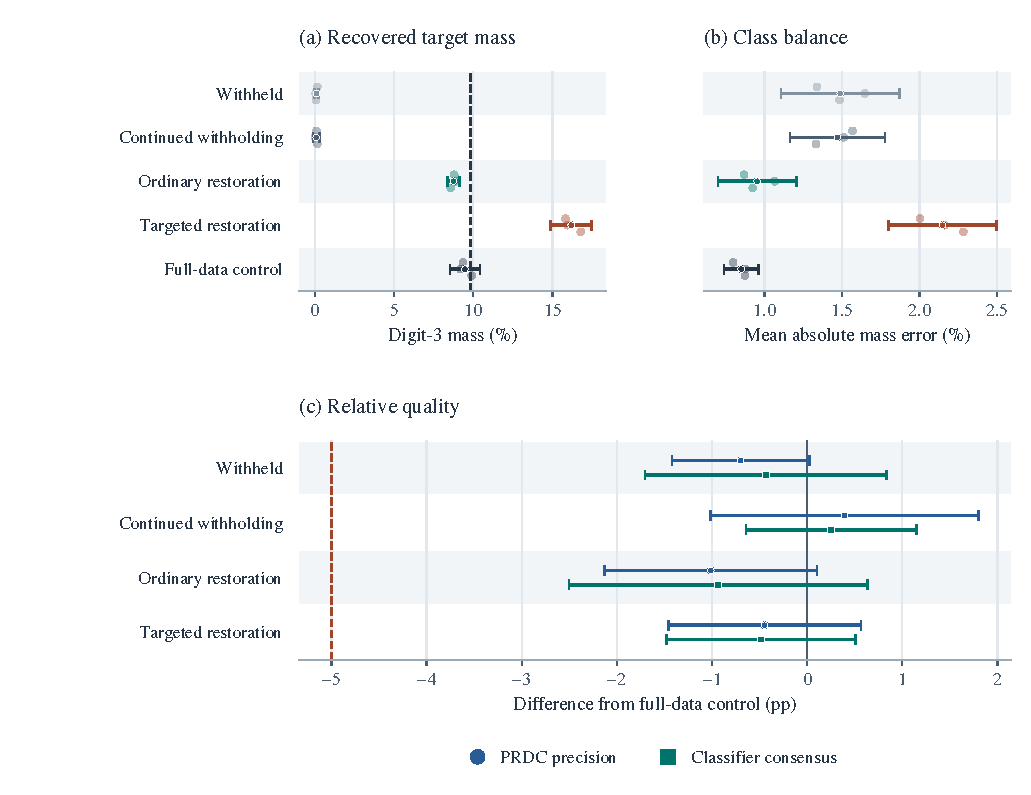
\includegraphics[width=\textwidth]{../figures/mnist_final_primary.pdf}
\caption{Completed original confirmation at DPM++25. All five checkpoint states
and the predeclared quality differences are retained. Small dots show
individual seed outcomes. Intervals are descriptive
95\% Student-$t$ intervals across three independent training seeds; the quality panel's dashed line is the
five-percentage-point noninferiority margin. Ordinary restoration improves
balanced support; targeted restoration overshoots the missing region.}
\label{fig:mnist_primary_supp}
\end{figure*}

\begin{figure*}[t]
\centering
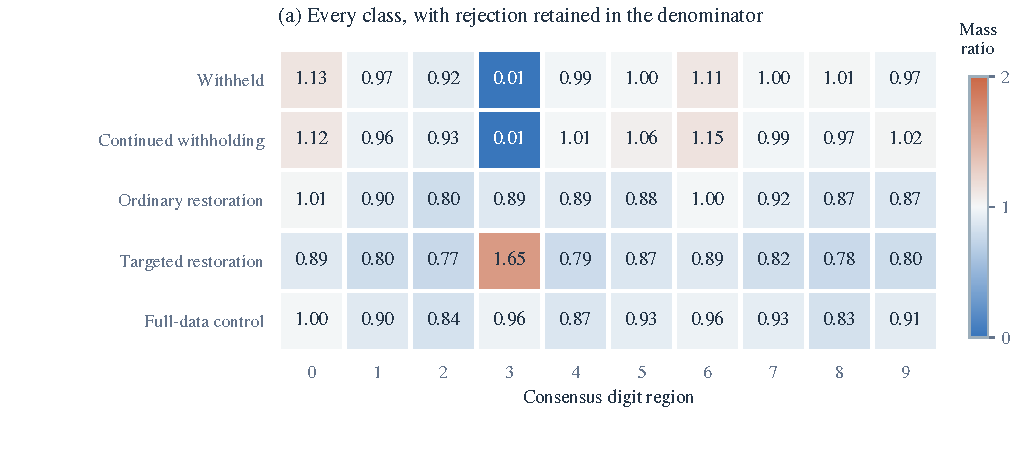
\includegraphics[width=\textwidth]{../figures/mnist_final_class_masses.pdf}
\caption{All ten consensus-region mass ratios relative to real data. This
complete class accounting exposes the targeted intervention's overcorrection.
Rejected samples remain in the denominator; class probabilities are not
renormalized over accepted images.}
\label{fig:mnist_masses_supp}
\end{figure*}

\begin{figure*}[t]
\centering
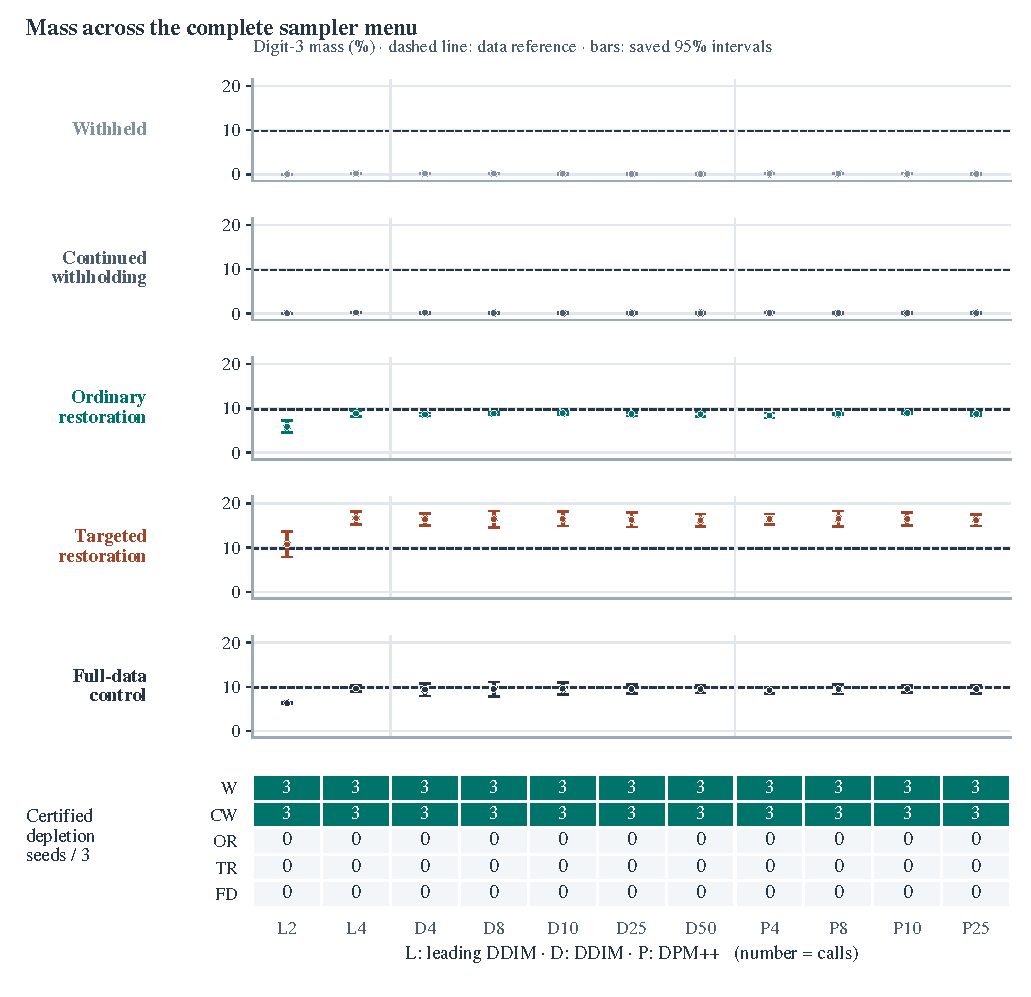
\includegraphics[width=\textwidth]{../figures/mnist_final_solver_persistence.pdf}
\caption{Complete sampler comparison from the original frozen study.
The missing region persists at resolved step budgets under both DDIM and
DPM++, while ordinary data restoration improves its mass. Intervals are
descriptive 95\% Student-$t$ intervals across three training seeds and do not
treat generated panels as independent models.}
\label{fig:mnist_persistence_supp}
\end{figure*}

\begin{figure*}[t]
\centering
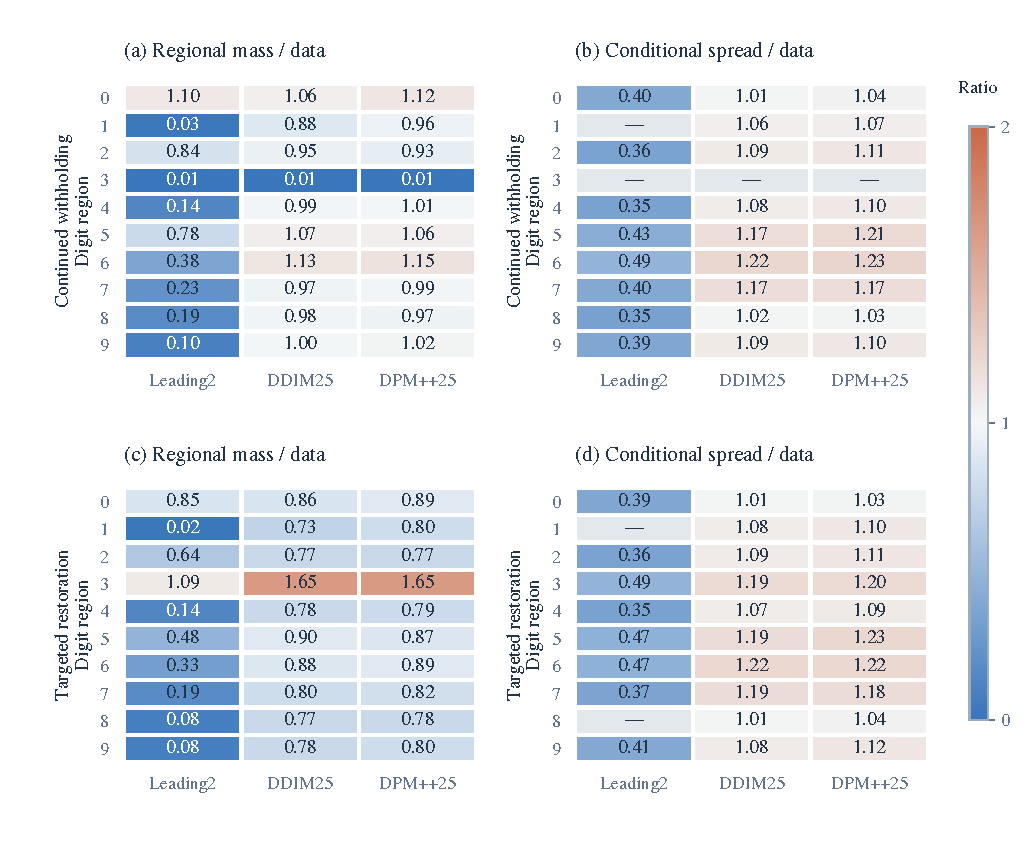
\includegraphics[width=\textwidth]{../figures/mnist_final_mixed_mechanisms.pdf}
\caption{Secondary conditional-spread measurements in independently fitted
PCA32 coordinates and validated semantic cells. Minimum counts and all
ineligible cells are retained. Displayed values are point ratios. Complete interval-based statuses use the
approximate influence-function construction with the declared 1,650-cell
family; they are not exact certificates.}
\label{fig:mnist_mixed_supp}
\end{figure*}

\begin{figure*}[t]
\centering
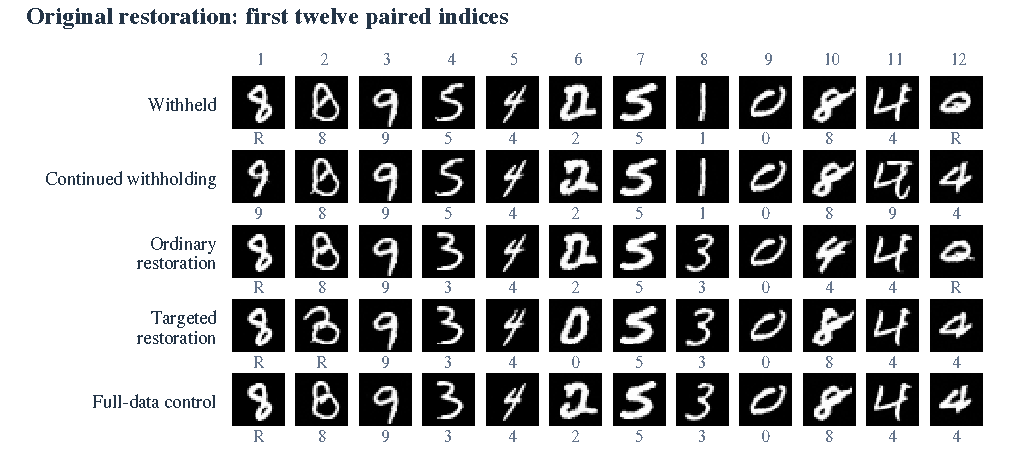
\includegraphics[width=\textwidth]{../figures/mnist_final_qualitative.pdf}
\caption{First twelve noise indices from training seed 10 under DPM++25,
paired across every checkpoint state. No example is ranked or excluded.
Annotations beneath the images show the fixed classifier-consensus digit or rejection; they
allow inspection of the measurement and do not replace visual fidelity.}
\label{fig:mnist_qualitative_supp}
\end{figure*}

\subsection{Signed mass supports an equal-update repair of overcorrection}
\label{sec:mnist_balance_supp}
Ordinary continuation reduces ten-class mass error by 58.7\% and target-digit
absolute error by 89.1\% relative to continued targeting at equal update
budget. This separate follow-up uses a two-sided mass audit to identify
excess probability even when every digit remains represented. Its audit and
matched-update comparison were frozen before follow-up training or generation.
The original restoration results and the 30 crossed-probe routing decisions
(Sec.~\ref{supp:mnist_routing}) remain unchanged. The controlled comparison
tests a repair of measured imbalance without identifying a unique historical cause.

\paragraph{Matched training branches and fresh evaluation.}
Each of the three targeted-restoration checkpoints branches into two further
8,000-update runs. Ordinary continuation draws uniformly from the 60,000
training images. Continued targeted sampling draws from the same images plus
one duplicate of each of the 6,131 digit-3 training images. Both branches
start from identical model, EMA, AdamW, and CUDA random states; the global EMA
counter continues from 33,000 to 41,000 updates. Branch receipts verify these
loaded states. Batch size, learning rate,
optimizer, precision, architecture, and loss are unchanged. No evaluation
occurs during training. The original 33,000-update full-data models are
fixed fidelity controls, not equal-update intervention branches.

All four checkpoint states---targeted parent, ordinary continuation, targeted
continuation, and full-data control---are evaluated under trailing DDIM25,
trailing DDIM50, and second-order DPM++25 for all three training seeds.
Each of these 36 arms receives 16,000 diagnosis samples and 2,000 independent
outcome samples. Noise seeds are paired across arms and are disjoint from
every earlier study. All diagnosis artifacts and their complete decisions
are saved and hashed before outcome generation. Semantic probabilities use
the same frozen classifier-consensus event and all 10,000 real test images;
the denominator includes rejected images. Geometric fidelity retains the
disjoint 3,000/2,000/5,000 real fit/calibration/evaluation split.

\paragraph{Exact two-sided mass bounds.}
For each digit, let $p$ and $q$ be real and generated unconditional consensus
probabilities. We construct Clopper--Pearson intervals $[p_L,p_U]$ and
$[q_L,q_U]$, then report
\begin{equation}
  q-p\in[q_L-p_U,\;q_U-p_L].
\label{eq:supp_mnist_mass_difference}
\end{equation}
The mass error budget is $\alpha_m=0.025$. Half is allocated once across
the ten shared real-reference intervals, and half across all 360 generated
digit--arm intervals. Thus each reference tail has error
$\alpha_m/(4\cdot10)$ and each generated tail
$\alpha_m/(4\cdot360)$. A union bound gives simultaneous coverage at least
$1-\alpha_m$ for the declared differences, conditional on the fixed
semantic regions and trained models. Shared references and paired-noise
dependence across arms do not invalidate this bound.

At the prespecified absolute tolerance $\delta=0.03$, a class is excessive if
the difference interval lies above $\delta$, depleted if it lies below $-\delta$,
equivalent if it lies wholly within $[-\delta,\delta]$, and otherwise inconclusive.
Three percentage points is an explicit MNIST-scale practical resolution,
about 30\% of a nominal balanced class; it is not a universal semantic
threshold. Every class is retained, and the same intervals are evaluated
at $\delta=0.02$ and $0.04$ for sensitivity. Rejection is governed by fidelity,
not treated as a semantic digit.

Synthetic sample planning preceded training. Across 20,000 multinomial
trials per setting, 16,000 generated samples with the fixed-size 10,000-image
reference detect a digit-3 mass of 0.16 as excessive with 99.23\% probability
([99.10,99.35]\% Monte Carlo interval)
and certify all-ten-class equivalence at exactly matching probabilities
with 95.58\% probability ([95.29,95.86]\%). At a digit-3 mass of 0.087,
all-class equivalence power is only 45.12\% ([44.42,45.81]\%); inconclusive
decisions remain expected near the resolution boundary. These planning
calculations concern one sampler, not the three-probe intersection. Its
power also depends on dependence across probes. They are not measured model
performance.

\paragraph{Qualification and persistence.}
The two relative-fidelity events are membership in fixed real-fit
five-neighbor balls and classifier-consensus acceptance. All 27 non-control
arms are paired with the same-seed, same-sampler full-data control. The exact
paired Bernoulli construction in Sec.~\ref{supp:mnist_paired_quality} uses $\alpha_f=0.0125$ across 54 metric
comparisons and a five-percentage-point noninferiority margin. Full-data
self-comparisons are structural zero-difference reference anchors; they do
not establish absolute perceptual fidelity. A checkpoint receives a
persistent-imbalance decision only when at least one same digit is excessive
or depleted under all three resolved samplers and all their fidelity gates
pass. Balanced-at-resolution requires every digit to be equivalent under
all three samplers with the same qualification. All other outcomes are
inconclusive. The calibrated real-support tail is separately reported with
$\alpha_s=0.0125$ across 36 comparisons; it is not silently added as a third
qualification gate. The three exact families sum to 0.05. This simultaneous
statement does not include the approximate training-seed outcome intervals.

\paragraph{Prespecified independent outcomes.}
The two primary comparisons are ordinary minus targeted continuation under
DPM++25 for ten-class mean absolute mass error and digit-3 absolute mass
error. Each receives a 97.5\% paired Student-$t$ interval across the three
training seeds (Bonferroni correction for two comparisons, two degrees of
freedom). These intervals assume approximately normal seed effects and
condition on the common fixed real reference. All other sampler, class,
coverage, precision, support, and variance measurements are reported with
descriptive uncertainty. Four five-percentage-point fidelity constraints
compare ordinary continuation with both continued targeting and the
full-data control for the two declared events; the conjunction passes only
if every paired 95\% interval has lower bound at least $-0.05$.
The 2,000-image outcomes issue no new semantic certificates and do not tune
thresholds, select a sampler, or change diagnosis decisions.

\paragraph{Complete frozen diagnosis.}
The signed audit certifies persistent digit-3 excess in all three targeted
parents and all three continued-targeting checkpoints at $\delta=0.03$.
Digit~3 is equivalent within the same tolerance in all nine ordinary-
continuation probe arms and all nine full-data probe arms. Thus the
specifically identified regional excess is resolved at the declared
resolution, while broader balance remains a separate question.
Every non-control arm passes both relative-fidelity gates (27/27), while
the nine full-data arms retain their explicit anchor status. Ordinary
continuations and full-data controls are all inconclusive for all-ten-class
balance at this resolution; none is labeled data-adequate. At $\delta=0.04$,
ordinary and full-data checkpoints from seeds 10 and 11 receive equivalence
certificates, while both seed-12 checkpoints remain inconclusive. The
seed-10 targeted parent becomes inconclusive for excess at this larger
margin; the other five targeted checkpoints retain persistent excess.
At $\delta=0.02$, the six targeted checkpoints retain excess and the other six
remain inconclusive. Table~\ref{tab:mnist_balance_diagnosis} includes every
checkpoint and sensitivity decision.

The separate support-tail gate passes in 34 of 36 arms. Its two inconclusive
cases are seed-10 targeted-parent DDIM50 and seed-11 full-data DDIM50, with
excess-tail differences 0.03129 [0.01047,0.05085] and
0.03066 [0.00987,0.05020], respectively, against the 0.05 margin.
Neither is a support failure, and neither is silently counted as a pass.
An independent reconstruction of raw semantic counts, paired-fidelity
discordances, support events, and all declared interval/decision formulas
matches the saved diagnosis in all 653 numerical comparisons.

\begin{table*}[t]
\centering\small
\caption{Every signed-mass checkpoint decision. E/D denotes persistent excess/depletion of the listed digit across all three resolved samplers; B denotes all-ten-digit equivalence at the stated resolution; ? denotes inconclusive. Fidelity lists the two-gate conjunction for DDIM25/DDIM50/DPM++25: P (pass), F (fail), I (inconclusive), A (structural reference anchor). Anchors do not certify absolute quality. The primary absolute mass tolerance is $\delta=0.03$; the other columns use the same bounds for prespecified sensitivity analysis.}
\label{tab:mnist_balance_diagnosis}
\begin{tabular}{llcccc}
\toprule
Checkpoint & Seed & Fidelity (25/50/DPM) & $\delta=0.02$ & $\delta=0.03$ & $\delta=0.04$ \\
\midrule
Targeted parent & 10 & P/P/P & E(3) & E(3) & ? \\
Ordinary continuation & 10 & P/P/P & ? & ? & B \\
Targeted continuation & 10 & P/P/P & E(3) & E(3) & E(3) \\
Full-data anchor & 10 & A/A/A & ? & ? & B \\
Targeted parent & 11 & P/P/P & E(3) & E(3) & E(3) \\
Ordinary continuation & 11 & P/P/P & ? & ? & B \\
Targeted continuation & 11 & P/P/P & E(3) & E(3) & E(3) \\
Full-data anchor & 11 & A/A/A & ? & ? & B \\
Targeted parent & 12 & P/P/P & E(3) & E(3) & E(3) \\
Ordinary continuation & 12 & P/P/P & ? & ? & ? \\
Targeted continuation & 12 & P/P/P & E(3) & E(3) & E(3) \\
Full-data anchor & 12 & A/A/A & ? & ? & ? \\
\bottomrule
\end{tabular}
\end{table*}


\paragraph{Independent outcomes and retained tradeoffs.}
Both prespecified primary comparisons favor ordinary continuation.
At DPM++25, ten-class mass error is 0.00900 versus 0.02177 for continued
targeting; the paired difference is $-0.01277$
[$-0.01878,-0.00676$]. Digit-3 absolute error is 0.00747 versus 0.06837,
with difference $-0.06090$ [$-0.11814,-0.00366$]. These are the two
97.5\% adjusted three-seed intervals. The corresponding class-3 masses are
0.09083 and 0.16667 against the real reference's 0.0983. The complete
DDIM25 and DDIM50 comparisons agree in direction: ordinary-minus-targeted
mass-error changes are $-0.01268$ [$-0.01546,-0.00990$] and
$-0.01227$ [$-0.01551,-0.00903$], and class-3 absolute-error changes are
$-0.06173$ [$-0.09812,-0.02534$] and
$-0.06140$ [$-0.09922,-0.02358$]. These secondary intervals are descriptive
95\% intervals, without a simultaneous all-sampler claim.

The four primary fidelity constraints pass. Ordinary-minus-targeted
fixed-neighborhood precision is $+0.00650$ [$-0.00336,0.01636$], while
consensus acceptance changes by $-0.00617$ [$-0.02481,0.01248$].
Against full-data controls, the corresponding changes are $+0.00683$
[$-0.00388,0.01754$] and $+0.00117$ [$-0.03085,0.03318$]. Every lower
bound exceeds $-0.05$. Ordinary continuation has consensus acceptance
0.87383, versus 0.88000 for continued targeting, 0.87267 for full-data
controls, and 0.95460 for real data. The relative-fidelity comparison does
not erase this real/generated difference. Classifier rejection contributes
to the unresolved all-class balance shown in
Fig.~\ref{fig:mnist_balance_allclass}.

Conventional PRDC yields additional, less decisive comparisons. At DPM++25,
ordinary-minus-targeted precision is $-0.00600$ [$-0.02111,0.00911$], and
coverage is $+0.00393$ [$-0.02911,0.03698$]. Thus the mass repair does not
establish broad quality or coverage superiority. PRDC uses the independent
5,000-image real evaluation pool against 2,000 generated outcomes; fixed-
neighborhood precision instead uses 3,000 real-fit anchors. Neither is the
original 165-arm study's five disjoint 1,000-image PRDC panels, so these
absolute values should not be compared across studies without that distinction.
Table~\ref{tab:mnist_balance_all} and the result files retain all 36 arms,
every class, all six checkpoint-pair comparisons under each sampler, and
their three-seed intervals.

\paragraph{Compute and verification.}
The six branches use 48,000 new optimizer updates, or 6.144 million training
batch examples. Three paired workers complete training in approximately
22.4 minutes while sharing an H200; their summed elapsed times are 4,028.7
seconds and are not an exclusive-GPU measurement. Diagnosis generates
576,000 images using 19.2 million denoiser-image calls; independent outcomes
generate 72,000 images using 2.4 million calls. Recorded sampling times are
882.5 and 113.9 seconds, respectively, and CPU diagnosis takes 79.7 seconds.
Per checkpoint, the audit requires 48,000 diagnosis images and 1.6 million
calls across three probes. It is an amortizable checkpoint audit, not a
cheap per-image operation. Generation moves to the second H200 only after
an unrelated old-checkpoint parity check produces exactly identical images,
features, and probabilities on both devices, with all numerical settings
unchanged. Timing is descriptive under concurrent workloads.

The manifest verifies all 72 archives, checkpoint/protocol identities, and
paired seeds. Independent reconstruction matches all 1,661 outcome
comparisons, including PRDC, within $1.78\times10^{-15}$.
Figure~\ref{fig:mnist_balance_grid} retains every state's first twelve
paired outcome seeds.

\begin{table*}[t]
\centering\small\setlength{\tabcolsep}{4pt}
\caption{Complete balance-follow-up outcome comparisons. Mean $\pm$ descriptive 95\% across-training-seed interval half-width ($n=3$); mass metrics use the same 10,000-image semantic reference. Fixed-reference precision uses the original 3,000 real feature anchors. The ordinary and targeted continuation branches each receive 8,000 additional updates from identical targeted parents. Full unrounded endpoints are retained in the result files.}
\label{tab:mnist_balance_all}
\begin{tabular}{llrrrr}
\toprule
Checkpoint & Sampler & Digit-3 mass & Mass MAD $\downarrow$ & Fixed precision $\uparrow$ & Consensus $\uparrow$ \\
\midrule
Targeted parent & DDIM25 & $0.1597\pm0.0268$ & $0.0224\pm0.0064$ & $0.8855\pm0.0120$ & $0.8537\pm0.0186$ \\
Targeted parent & DDIM50 & $0.1592\pm0.0267$ & $0.0216\pm0.0070$ & $0.8845\pm0.0164$ & $0.8618\pm0.0136$ \\
Targeted parent & DPMPP25 & $0.1597\pm0.0225$ & $0.0209\pm0.0044$ & $0.8803\pm0.0134$ & $0.8687\pm0.0029$ \\
Ordinary continuation & DDIM25 & $0.0910\pm0.0087$ & $0.0106\pm0.0048$ & $0.8967\pm0.0133$ & $0.8578\pm0.0318$ \\
Ordinary continuation & DDIM50 & $0.0912\pm0.0148$ & $0.0098\pm0.0046$ & $0.8972\pm0.0107$ & $0.8670\pm0.0305$ \\
Ordinary continuation & DPMPP25 & $0.0908\pm0.0121$ & $0.0090\pm0.0047$ & $0.8965\pm0.0126$ & $0.8738\pm0.0320$ \\
Targeted continuation & DDIM25 & $0.1673\pm0.0284$ & $0.0233\pm0.0054$ & $0.8923\pm0.0047$ & $0.8640\pm0.0281$ \\
Targeted continuation & DDIM50 & $0.1668\pm0.0252$ & $0.0221\pm0.0063$ & $0.8920\pm0.0126$ & $0.8765\pm0.0200$ \\
Targeted continuation & DPMPP25 & $0.1667\pm0.0298$ & $0.0218\pm0.0074$ & $0.8900\pm0.0062$ & $0.8800\pm0.0209$ \\
Full-data control & DDIM25 & $0.0962\pm0.0155$ & $0.0113\pm0.0024$ & $0.8905\pm0.0037$ & $0.8537\pm0.0137$ \\
Full-data control & DDIM50 & $0.0963\pm0.0187$ & $0.0105\pm0.0038$ & $0.8948\pm0.0115$ & $0.8685\pm0.0218$ \\
Full-data control & DPMPP25 & $0.0932\pm0.0127$ & $0.0098\pm0.0034$ & $0.8897\pm0.0117$ & $0.8727\pm0.0093$ \\
\bottomrule
\end{tabular}
\end{table*}


\begin{figure*}[t]
\centering
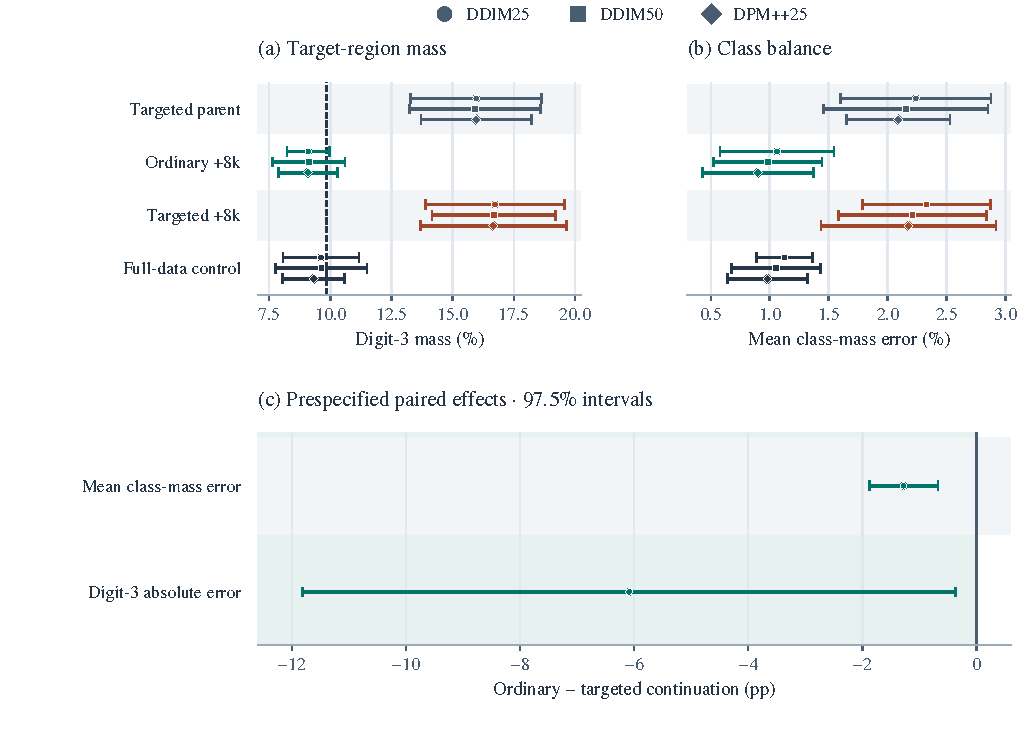
\includegraphics[width=\textwidth]{../figures/mnist_balance.pdf}
\caption{Complete balanced-restoration outcome comparisons.
(a,b) All four checkpoint states and all three resolved samplers, with
descriptive 95\% intervals across three training seeds. The dashed line is
the real digit-3 consensus mass.
(c) Both prespecified DPM++25 differences with 97.5\% paired intervals
(two-comparison adjustment). Intervals condition on the shared fixed real
reference and use the approximate three-seed Student-$t$ model.}
\label{fig:mnist_balance_results}
\end{figure*}

\begin{figure*}[t]
\centering
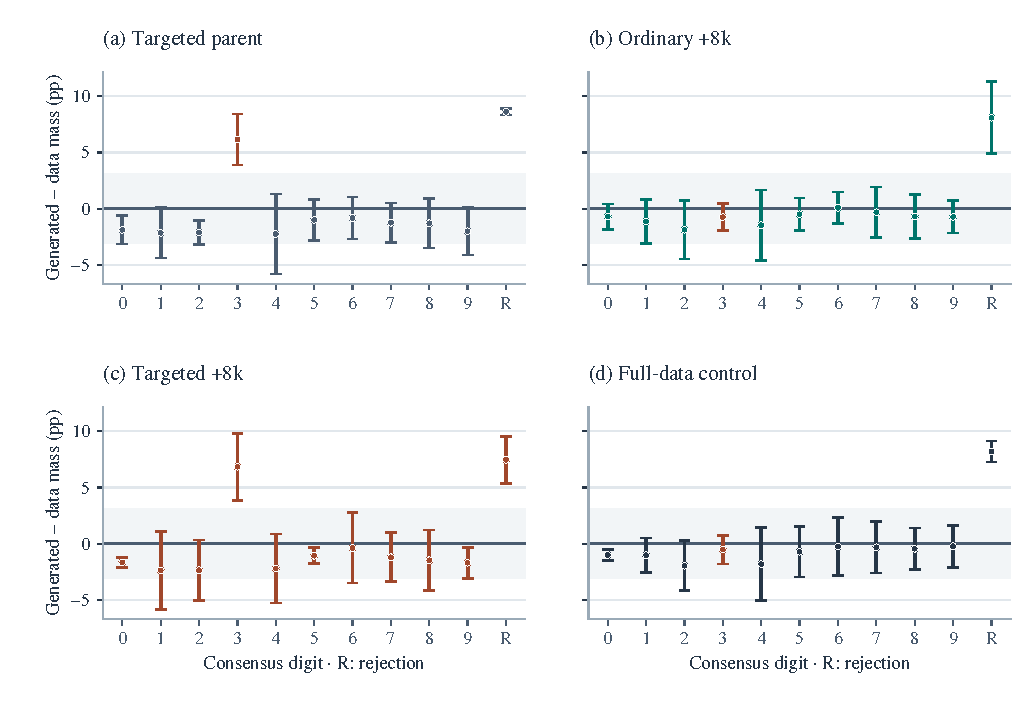
\includegraphics[width=\textwidth]{../figures/mnist_balance_allclass.pdf}
\caption{Every class and the rejection cell at the prespecified DPM++25
sampler. Points are generated-minus-real unconditional masses; intervals
are descriptive 95\% Student-$t$ intervals across three seeds. Digit~3 is
highlighted; the pale band marks the $\pm3$ percentage-point tolerance for
context. These outcome intervals are distinct from the exact diagnosis
bounds. Ordinary continuation resolves the targeted digit's excess while
other regional differences and excess rejection remain visible.}
\label{fig:mnist_balance_allclass}
\end{figure*}

\begin{figure*}[t]
\centering
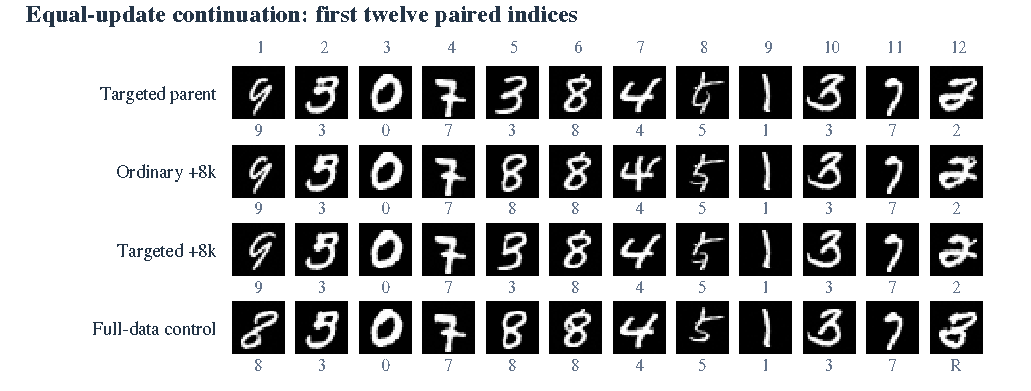
\includegraphics[width=\textwidth]{../figures/mnist_balance_qualitative.pdf}
\caption{Uncurated balanced-restoration outcomes: the first twelve fresh
DPM++25 noise seeds for training seed 10, paired across all four checkpoint
states. The two continuation branches each receive 8,000 updates from the
same targeted parent. The separately trained full-data model is a quality
control. Ambiguous images remain in the grid; none is selected by quality
or classifier label.}
\label{fig:mnist_balance_grid}
\end{figure*}

\begin{figure}[t]
\centering
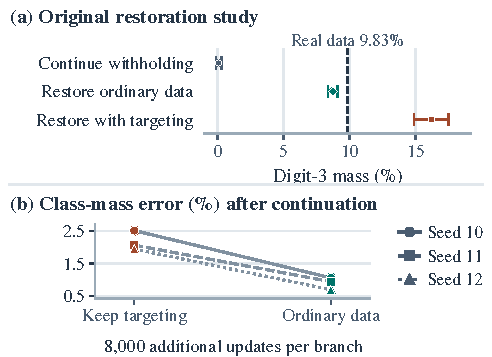
\includegraphics[width=\linewidth]{../figures/mnist_actionable.pdf}
\par\smallskip{\small
\setlength{\tabcolsep}{2.2pt}
\begin{tabular*}{\linewidth}{@{\extracolsep{\fill}}lrrrrr@{}}
\toprule
& \multicolumn{3}{c}{(a) Digit-3 mass (\%)}
& \multicolumn{2}{c@{}}{(b) Class-mass error (\%)} \\
\cmidrule(lr){2-4}\cmidrule(l){5-6}
Seed & Withheld & Ordinary & Targeted & Targeted & Ordinary \\
\midrule
10 & $0.100$ & $8.800$ & $15.820$ & $2.515$ & $1.062$ \\
11 & $0.000$ & $8.860$ & $15.940$ & $2.065$ & $0.946$ \\
12 & $0.160$ & $8.580$ & $16.780$ & $1.950$ & $0.691$ \\
\midrule
Mean & $0.087$ & $8.747$ & $16.180$ & $2.177$ & $0.900$ \\
\bottomrule
\end{tabular*}
}

\caption{Signed measurements support a verified repair of overcorrection.
Both panels use DPM++25. (a) Original ordinary restoration recovers missing
digit-3 mass; targeted restoration overshoots the real-data target (dashed
line). Whiskers show ordinary 95\% Student-$t$ intervals over three training
seeds. (b) A separately frozen follow-up compares equal 8,000-update branches
from each targeted parent. Lines join outcomes from the same seed.
The table gives seed-level values and means.}
\label{fig:mnist_actionable}
\end{figure}

\subsection{Crossed numerical and data probes}
\label{supp:mnist_routing}
The original experiment crosses five checkpoint states with eleven samplers.
We additionally freeze a prospective routing evaluation before generating new
samples. It reuses the three trained seeds and all five states, with leading
DDIM2, trailing DDIM4/25/50, and DPM++25. Each of these 75 arms generates
8,000 diagnosis images and then 2,000 independent outcome images. Every
image uses noise seed $71{,}000{,}000+100{,}000s+i$, with indices 0--7,999
for diagnosis and 8,000--9,999 for outcomes; indices are paired across states
and samplers. All diagnostic routes and policy actions are saved before any
outcome generation begins. No checkpoint is trained further for this study.

\paragraph{Two references and fixed measurements.}
For each short sampler, the same checkpoint's DPM++25 output is its
teacher-relative reference. The data reference uses the final 5,000 real test
images; the first 3,000 fit the geometry and the next 2,000 calibrate its
support threshold. Semantic regions remain the validated classifier-consensus
cells. A fixed real-neighborhood precision event accepts a generated feature
inside the union of real-fit feature balls, each with its fifth-neighbor
radius. This makes each image's precision indicator independent of other
generated images, enabling a paired Bernoulli interval. It differs from
sample-dependent recall and coverage; complete conventional PRDC metrics are
also reported on outcomes.
The fresh outcome PRDC compares 2,000 generated images against all 5,000
reference-evaluation images. This differs from the original study's five
1,000-by-1,000 PRDC panels and its 10,000-image semantic reference. Fresh
semantic masses use only the 5,000 evaluation reference images. Consequently,
absolute nearest-neighbor metrics and finite-reference class masses should
not be compared across the two protocols as if their evaluation sets matched.

\paragraph{Exact paired quality intervals.}\label{supp:mnist_paired_quality}
For each shared-noise pair, let $D=I_{\rm candidate}-I_{\rm reference}$
for consensus acceptance or fixed real-neighborhood precision. Write
$\eta=\Pr(D\ne0)$ and $\pi=\Pr(D=1\mid D\ne0)$. Then the quality
difference is $\Delta=\eta(2\pi-1)$. Clopper--Pearson intervals for
$\eta$ and $\pi$, with tail error $\alpha/(4M)$, give a rectangle;
the minimum and maximum of $\eta(2\pi-1)$ over its four corners bound
$\Delta$. Conditional binomial coverage holds for every random discordance
count, so a union bound proves simultaneous coverage over the declared family.
For zero discordances, the conditional interval is $[0,1]$, giving
$[-\eta^+,\eta^+]$. Both quantities are bounded rather than substituting
a potentially invalid plug-in discordance estimate~\cite{newcombe1998paired};
we do not propose a new paired-proportion estimator.
The same finite-sample calculation is applied to full-data identity controls.
Noninferiority passes only when the lower bound is at least $-0.05$.
Synthetic multinomial simulations and an independent implementation validate
coverage, boundary behavior, and interval arithmetic before learned-model
sampling. At 8,000 pairs, 20,000 synthetic trials with reference acceptance 0.85,
a $-0.01$ difference, and discordance 0.255 give 99.17\% passing probability
(95\% simulation interval 99.03--99.29\%). A $-0.025$ difference gives only
37.91\% power: acceptable differences nearer the margin can remain inconclusive.

\paragraph{Frozen families and route.}
The semantic family contains 1,155 cells: 30 short/data, 30 short/teacher,
and 45 resolved/data comparisons, each with eleven cells and total error
0.025. The paired fidelity family has 150 metric comparisons: the 45 resolved
arms against full-data at the same sampler, plus the 30 short/teacher pairs,
each with two metrics and error 0.0125. Separately, 75 absolute data-support
and 30 paired teacher-support comparisons share error 0.0125. These three
exact families sum to 0.05. Conditional spread uses 300 separately labeled
approximate intervals, one per digit in each short/teacher pair, in unwhitened
PCA32 coordinates. Its paired influence function preserves shared-noise
covariance even when the two samples enter different semantic cells.

A resolved probe is adequate only if both fidelity metrics pass relative to
the corresponding full-data sampler. A data route requires the same digit's
certified depletion under all three resolved probes and adequacy of all three.
A numerical route requires an adequate DPM++25 teacher and short/teacher
regional depletion, conditional contraction, fidelity failure, or support-tail
failure. Both signals produce a combined route; neither yields inconclusive.
Reject-cell depletion does not establish a missing semantic region. Absolute
real-support flags remain visible, including defects shared by the full-data
benchmark; they are not silently promoted to an additional eligibility test.
Because numerical routing can use approximate spread intervals, the entire
routing decision is not an exact 95\% certificate. These are qualified
recommendations for intervention tests, not unique causal identifications.

\paragraph{All policies and independent outcomes.}
For the six original-withheld cases, available data interventions are precisely
the equal-8,000-update continuation branches. A numerical route chooses
continued withholding with DPM++25; a data route chooses ordinary restoration
with the original short sampler; a combined route chooses ordinary restoration
with DPM++25. An inconclusive route uses the continued-withheld short control.
Thus the policy named ``no change'' denotes matched additional training on
withheld data, not the unchanged 25,000-update origin. Comparators are this
control, occupancy-only routing, always numerical, always data, always
combined, targeted restoration at the short sampler, and targeted restoration
with DPM++25. Occupancy-only chooses ordinary restoration whenever any baseline
data-relative digit deficit is certified. All eight policies and all 75 outcome
arms are reported. For every one of the 30 crossed cases we also report the
short-to-DPM++25 outcome change, without inventing a new training transition
from checkpoints that already received restoration.
Numerical repair increases inference cost from 2 or 4 calls to 25; these
comparisons measure the benefit of resolving the sampler, not a free or
matched-budget gain.

Policy intervals average the two short settings within each trained seed,
then use paired Student-$t$ intervals over three seeds. They condition on the
shared real reference and assume approximately normal training-seed effects;
there is no simultaneous superiority claim over policies. The diagnostic
cost is substantial: 600,000 images and 12.72 million denoiser calls across
15 checkpoints, followed by 150,000 independent outcome images. This is a
checkpoint-level audit whose cost can be amortized over deployment, not a
cheap per-prompt diagnostic.
The 8,000 diagnosis samples are per sampler arm: across five samplers this is
40,000 images and 848,000 denoiser-image calls per checkpoint.

\subsection{Crossed-probe outcomes and limits}
All 150 diagnosis/outcome files passed configuration, row-count, pairing,
checkpoint-hash, and sample-checksum validation. The 30 routes were frozen
before any outcome generation. All three resolved probes pass both declared
quality constraints in every checkpoint. The twelve short-sampler cases from
withheld or continued-withheld checkpoints retain the same deficient digit~3
under all three probes and receive the combined route. The eighteen cases from
ordinary restoration, targeted restoration, or full-data training have no
qualified persistent digit depletion and receive the numerical recommendation, which does not certify balanced mass. Training
absence or restoration labels are never inputs to the routing computation.

Occupancy-only routing raises a data flag in nine of the eighteen latter
cases, compared with zero persistent-reference depletion flags. This is a disagreement
in recommendations relative to the known training intervention, not a
classification accuracy or false-positive certificate: targeted restoration,
for example, changes other class probabilities and overrepresents digit~3.
Table~\ref{tab:mnist_all_routes} retains every decision and actual digit counts.
All 30 cases also have exact relative-fidelity evidence for their numerical
signal, although the general rule admits the separately approximate spread
test. No inconclusive outcome occurred in these particular checkpoints;
the implementation and synthetic controls retain that outcome.

The independent short-to-DPM++25 comparison improves class-mass error,
coverage, and consensus acceptance in every one of the eighteen
numerical-only cases. Across ordinary-restored, targeted, and full-data
checkpoints, mean mass-error changes are respectively $-0.05022$, $-0.03783$,
and $-0.05097$ from leading DDIM2, and $-0.01781$, $-0.01772$, and $-0.01804$
from trailing DDIM4. Precision has a meaningful tradeoff: fixed-neighborhood
membership improves from the two-call sampler but decreases from trailing
DDIM4 by 0.01133, 0.02150, and 0.01950, respectively. All 75 arms and all
30 paired changes, including their three-seed intervals, remain in the result
files. These observed numerical improvements use existing checkpoints. They do not
establish that all eighteen checkpoints need no data intervention: the six
targeted-checkpoint cases retain excess digit-3 mass, which the depletion-only
rule does not test. Of the nine nonpersistent occupancy flags, three come
from leading-DDIM2 targeted cases with this distinct imbalance. We therefore
do not count nine correct avoided training interventions or claim measured
counterfactual training savings.

For the six original-withheld origins, the audit chooses ordinary restoration
plus DPM++25 and therefore equals always-combined exactly. Its digit-3 mass is
$0.08567\pm0.01120$, versus $0.00067\pm0.00072$ for numerical repair alone.
Mass error is $0.01162\pm0.00117$, versus $0.04563\pm0.00191$ for data-only
repair and $0.01493\pm0.00379$ for numerical-only repair. Audit-minus-numerical
mass error is $-0.00331$ [$-0.00683,0.00020$], so superiority on this endpoint
is unresolved. Audit-minus-data-only error is $-0.03402$
[$-0.03555,-0.03248$]. Targeted restoration plus DPM++25 again overshoots,
with digit-3 mass 0.1650 and error 0.02348. All eight policies are retained in
Table~\ref{tab:mnist_routing_policies}; these are descriptive paired
three-training-seed comparisons, not a simultaneous best-policy claim.

Sampling takes 924.8 seconds for diagnosis and 221.1 seconds for outcomes;
CPU routing and outcome measurement take approximately 86 and 188 seconds.
No additional training is performed. Figure~\ref{fig:mnist_routing_grid_supp}
retains the first twelve fresh outcome noise indices from seed 10 for every
listed arm, including classifier rejections.

\begin{table*}[t]
\centering\small
\setlength{\tabcolsep}{4pt}
\caption{Fresh routing outcomes. All policies were frozen on independent diagnosis seeds. Mean $\pm$95\% Student-$t$ interval over three trained seeds, averaging the two short settings within each seed. Precision uses the fixed real-neighborhood event. Continued withholding is the matched 8,000-update control. These complete secondary comparisons do not assert simultaneous policy superiority.}
\label{tab:mnist_routing_policies}
\begin{tabular}{lrrrrr}
\toprule
Policy & Digit-3 mass & Mass error $\downarrow$ & Precision $\uparrow$ & Consensus $\uparrow$ & Calls \\
\midrule
Audit & $0.086\pm0.011$ & $0.012\pm0.001$ & $0.894\pm0.009$ & $0.865\pm0.025$ & $25.0$ \\
Occupancy only & $0.076\pm0.013$ & $0.046\pm0.002$ & $0.868\pm0.007$ & $0.517\pm0.019$ & $3.0$ \\
Numerical & $0.001\pm0.001$ & $0.015\pm0.004$ & $0.905\pm0.020$ & $0.875\pm0.010$ & $25.0$ \\
Restore data & $0.076\pm0.013$ & $0.046\pm0.002$ & $0.868\pm0.007$ & $0.517\pm0.019$ & $3.0$ \\
Restore + numerical & $0.086\pm0.011$ & $0.012\pm0.001$ & $0.894\pm0.009$ & $0.865\pm0.025$ & $25.0$ \\
Targeted & $0.137\pm0.017$ & $0.051\pm0.001$ & $0.871\pm0.013$ & $0.534\pm0.023$ & $3.0$ \\
Targeted + numerical & $0.165\pm0.015$ & $0.023\pm0.002$ & $0.888\pm0.013$ & $0.867\pm0.016$ & $25.0$ \\
Continue withheld & $0.001\pm0.001$ & $0.045\pm0.001$ & $0.875\pm0.007$ & $0.527\pm0.008$ & $3.0$ \\
\bottomrule
\end{tabular}
\end{table*}

\begin{table*}[t]\centering\small
\setlength{\tabcolsep}{4pt}
\caption{All 30 fresh depletion-only routing cases. The occupancy flag uses short-sampler data-relative digit depletion; persistence requires the same digit under all three quality-qualified resolved probes. Digit-3 counts are paired short/DPM++25 counts, out of8,000 for diagnosis and2,000 for independent outcomes. N denotes a numerical recommendation and D a data recommendation; N does not certify balanced data-relative mass. Training-state names are reporting labels, not inputs to the rule.}
\label{tab:mnist_all_routes}
\begin{tabular}{llrrrrrrr}\toprule
State & Seed & Calls & Occupancy flag & Persistent flag & Route & Diagnosis 3 & Outcome 3 & $\Delta$ mass error \\\midrule
Withheld & 10 & 2 & 1 & 1 & N+D & 6/8 & 0/3 & -0.0460 \\
Withheld & 10 & 4 & 1 & 1 & N+D & 16/8 & 2/3 & -0.0133 \\
Continue & 10 & 2 & 1 & 1 & N+D & 6/6 & 1/1 & -0.0475 \\
Continue & 10 & 4 & 1 & 1 & N+D & 8/6 & 3/1 & -0.0155 \\
Restore & 10 & 2 & 1 & 0 & N & 509/710 & 140/172 & -0.0483 \\
Restore & 10 & 4 & 0 & 0 & N & 700/710 & 176/172 & -0.0183 \\
Targeted & 10 & 2 & 1 & 0 & N & 902/1312 & 243/344 & -0.0375 \\
Targeted & 10 & 4 & 0 & 0 & N & 1299/1312 & 337/344 & -0.0173 \\
Full & 10 & 2 & 1 & 0 & N & 524/746 & 146/170 & -0.0483 \\
Full & 10 & 4 & 0 & 0 & N & 727/746 & 191/170 & -0.0171 \\
Withheld & 11 & 2 & 1 & 1 & N+D & 9/8 & 2/3 & -0.0463 \\
Withheld & 11 & 4 & 1 & 1 & N+D & 23/8 & 3/3 & -0.0166 \\
Continue & 11 & 2 & 1 & 1 & N+D & 2/11 & 2/2 & -0.0448 \\
Continue & 11 & 4 & 1 & 1 & N+D & 19/11 & 5/2 & -0.0148 \\
Restore & 11 & 2 & 1 & 0 & N & 468/684 & 121/180 & -0.0514 \\
Restore & 11 & 4 & 0 & 0 & N & 682/684 & 194/180 & -0.0170 \\
Targeted & 11 & 2 & 1 & 0 & N & 809/1278 & 199/325 & -0.0378 \\
Targeted & 11 & 4 & 0 & 0 & N & 1312/1278 & 337/325 & -0.0175 \\
Full & 11 & 2 & 1 & 0 & N & 531/768 & 146/192 & -0.0527 \\
Full & 11 & 4 & 0 & 0 & N & 735/768 & 191/192 & -0.0191 \\
Withheld & 12 & 2 & 1 & 1 & N+D & 10/6 & 4/3 & -0.0481 \\
Withheld & 12 & 4 & 1 & 1 & N+D & 13/6 & 3/3 & -0.0144 \\
Continue & 12 & 2 & 1 & 1 & N+D & 8/9 & 1/1 & -0.0469 \\
Continue & 12 & 4 & 1 & 1 & N+D & 12/9 & 4/1 & -0.0134 \\
Restore & 12 & 2 & 1 & 0 & N & 541/702 & 115/162 & -0.0510 \\
Restore & 12 & 4 & 0 & 0 & N & 743/702 & 163/162 & -0.0180 \\
Targeted & 12 & 2 & 1 & 0 & N & 993/1358 & 211/321 & -0.0381 \\
Targeted & 12 & 4 & 0 & 0 & N & 1422/1358 & 321/321 & -0.0183 \\
Full & 12 & 2 & 1 & 0 & N & 543/784 & 113/192 & -0.0519 \\
Full & 12 & 4 & 0 & 0 & N & 834/784 & 187/192 & -0.0179 \\
\bottomrule\end{tabular}\end{table*}


\begin{figure*}[t]
\centering
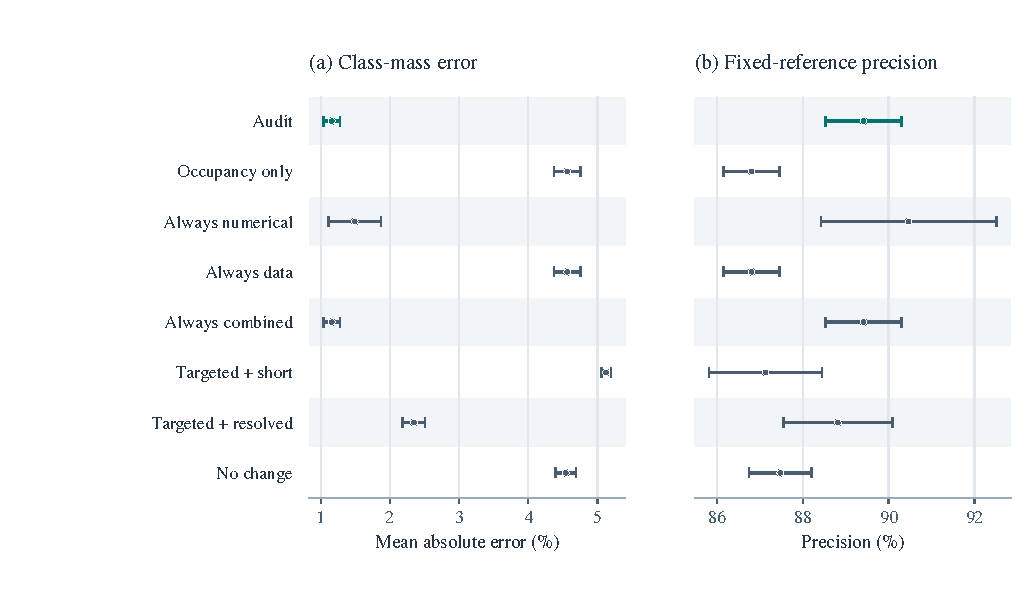
\includegraphics[width=\textwidth]{../figures/mnist_routing.pdf}
\caption{Complete independent outcomes of the depletion-only routing
study: all eight policies for six original-withheld origins. Both short settings
are averaged within each training seed; intervals are descriptive 95\%
Student-$t$ intervals over three seeds. (a) Mean absolute class-mass error.
(b) Membership in fixed real-fit five-neighbor balls. Numerical repair uses
25 calls versus the original 2/4; audit and always-combined coincide.
All 30 frozen recommendations remain in Table~\ref{tab:mnist_all_routes}.
A numerical recommendation does not certify balanced mass.}
\label{fig:mnist_routing}
\end{figure*}

\begin{figure*}[t]
\centering
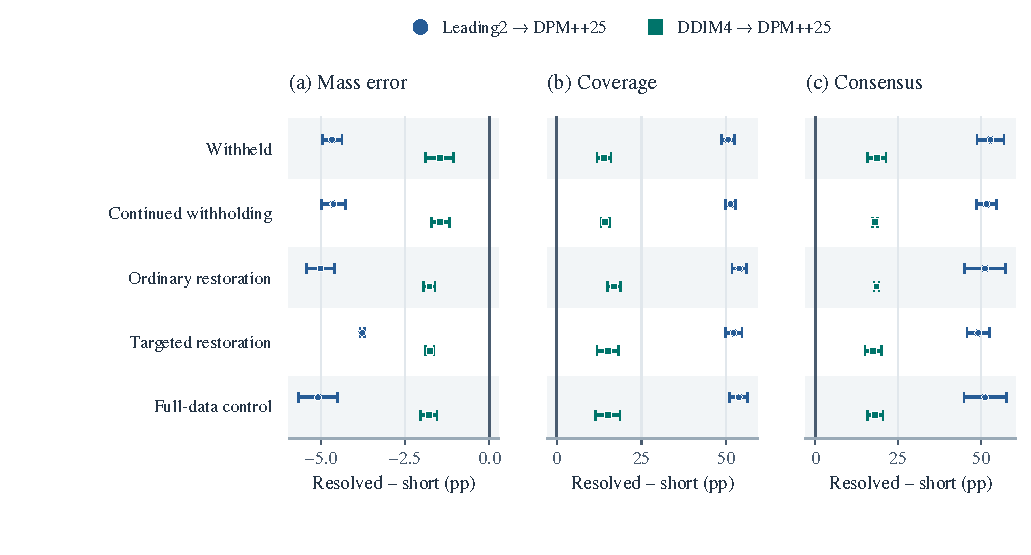
\includegraphics[width=\textwidth]{../figures/mnist_routing_numerical.pdf}
\caption{Every checkpoint state's independent short-to-resolved comparison.
All changes use the same checkpoint and paired fresh noise; intervals are
approximate 95\% paired Student-$t$ intervals across three trained seeds.
Numerical improvement cannot recover the withheld digit's data-relative mass;
restoration is needed for that deficit. Complete precision and support
outcomes accompany these plots in the saved result tables.}
\label{fig:mnist_routing_numerical_supp}
\end{figure*}

\begin{figure*}[t]
\centering
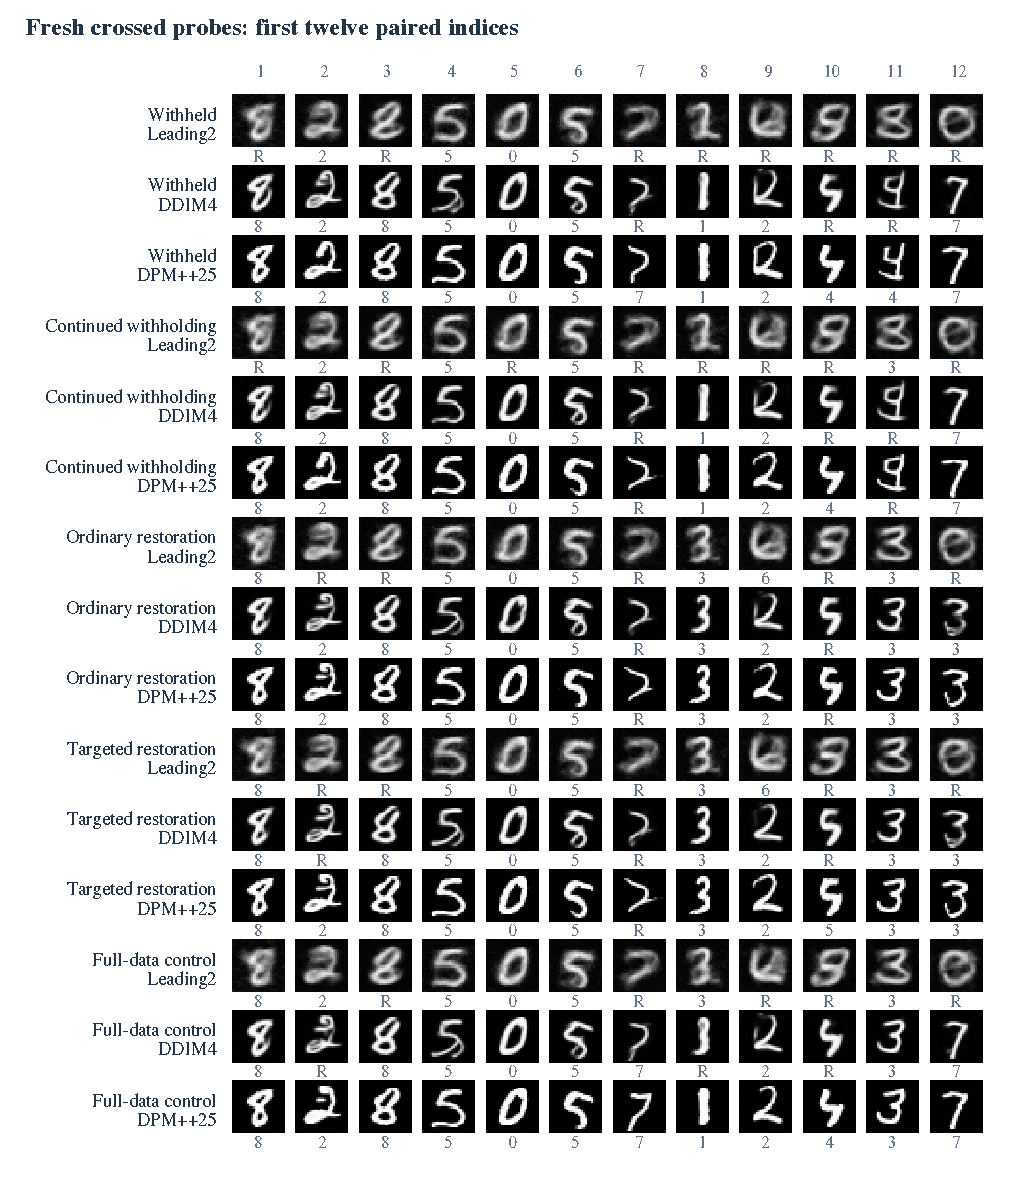
\includegraphics[width=\textwidth]{../figures/mnist_routing_qualitative.pdf}
\caption{Uncurated fresh outcomes: first twelve noise indices of training
seed 10, paired across all five checkpoint states and the two short samplers
plus DPM++25. Labels beneath the images are fixed classifier-consensus assignments or rejection.
Numerical resolution sharpens samples and increases acceptance; restored
data changes which semantic outcomes the checkpoint produces. Imperfect
digits and classifier disagreements remain visible.}
\label{fig:mnist_routing_grid_supp}
\end{figure*}

\section{Conditioning and reference matching resolve diversity reversals}
\label{sec:supp_t2i}

\subsection{Independent prompts, random streams, and evaluation units}
We use the complete public PartiPrompts~\cite{yu2022parti} prompt list, retaining its category and
challenge annotations. A fixed permutation (NumPy seed 20261015) selects 32
representation-fit prompts, 48 development prompts, 128 evaluation prompts, and
256 separate calibration prompts. Selection precedes generation and does not
inspect prompt wording or image outcomes. All 464 selected rows have unique
identifiers and unique casefolded, whitespace-normalized prompt strings, with
no exact text duplicate across splits. The reference fit pool contains 16
images per prompt; calibration uses one independently seeded image per prompt.
Development uses eight images per prompt. Evaluation uses eight diagnosis seeds
and 16 separate outcome seeds per prompt. All arm-level headline results use
only the 16 outcome seeds, giving 2,048 images per arm and 128 independent prompt
units. The eight diagnosis images implement a frozen action-selection rule;
they never enter the outcome estimate.

The initial seed is the split-specific offset plus 1,000 times the original
PartiPrompts row index plus the replicate index. Noise is drawn in CPU FP32 and
then converted to the model's native precision. Every method within a family
receives the same initial noise. Separate random streams, offset by $10^8$,
$2\!\times\!10^8$, and $3\!\times\!10^8$, supply stochastic scheduler updates,
conditional CADS perturbations, and unconditional CADS perturbations. The
Stable Diffusion evaluation offset is $10^7$; Sana uses $2\!\times\!10^7$.
The fit, calibration, development, and reference-refinement streams are disjoint
from evaluation. Saved configuration files list every prompt and seed; a
collision audit checks the generated initial-noise streams.

Let $p$ index the $N_{\rm p}$ evaluation prompts, and let $X$ and
$X_{\rm ref}$ denote candidate and reference images at that prompt.
For a representation $\phi$, the primary conditional spread ratio
uses sample covariances within prompts:
\begin{equation}
 R_\phi=\frac{N_{\rm p}^{-1}\sum_{p=1}^{N_{\rm p}}\operatorname{tr}
 \widehat{\operatorname{Cov}}(\phi(X)\mid p)}
 {N_{\rm p}^{-1}\sum_{p=1}^{N_{\rm p}}\operatorname{tr}
 \widehat{\operatorname{Cov}}(\phi(X_{\rm ref})\mid p)}.
\label{eq:supp_prompt_spread}
\end{equation}
Each prompt is centered separately and receives equal weight. This differs from
both a pooled covariance, which includes differences between prompts, and the
mean of promptwise variance ratios. We retain these alternatives as sensitivity
analyses. Intervals resample paired prompt units, preserving all seeds and all
methods within each sampled prompt. Arm and representation intervals are
descriptive 95\% intervals; the frozen policy's four primary contrasts use
98.75\% intervals. Fixed-prompt occupancy inference is kept separate from this
population-over-prompts analysis.
The saved representation analysis additionally retains an approximate simultaneous
95\% max-standardized-log-ratio bootstrap check across its 20 fixed contrasts.
A directional interval excluding 1 does not by itself pass the operational
0.9/1.1 contraction/expansion margins or the accompanying quality/support gates.

To explain a pooled/conditional reversal, we retain the exact balanced-design
ANOVA decomposition. With $N_{\rm p}$ prompts and $m$ samples per prompt,
let $W$ be the mean within-prompt sample covariance trace and $B_{\rm obs}$
the sample covariance trace of prompt means. The sample covariance trace
$T_{\rm pooled}$ across all images is
\begin{equation}
 T_{\rm pooled}=\frac{N_{\rm p}(m-1)}{N_{\rm p}m-1}W
              +\frac{m(N_{\rm p}-1)}{N_{\rm p}m-1}B_{\rm obs}.
\label{eq:supp_prompt_anova}
\end{equation}
We verify this identity numerically for every arm and representation. The
classical correction $B_{\rm obs}-W/m$ removes estimated finite-seed noise
from the prompt-mean covariance under independent seed draws; negative
estimates are retained. This is a descriptive variance-component analysis,
not a new estimator or a decision gate. The extension that retains both additive terms and this correction was
specified after access to the DDIM4 outcome contrast. It covers all 29 SD
and seven Sana arms using the same 128 prompts and 16 outcome seeds. The complete tables normalize both contributions by the common reference's
pooled trace and retain paired prompt-bootstrap intervals for between-prompt
ratios. For DINO, reference within/between contributions 0.400/0.600 become
0.523/0.396 under DDIM4. Their sum is the pooled ratio 0.919; dividing
within-prompt variation by the reference within component gives 1.306.
This secondary descriptive decomposition explains the reversal without
changing any primary comparison or gate.

\subsection{Native model configurations}
\paragraph{Stable Diffusion.}
All images are $512\!\times\!512$ pixels. The base model is SD1.5
\cite{rombach2022ldm}; DINOv2-base \cite{oquab2024dinov2} and CLIP ViT-L/14-336
\cite{radford2021clip} provide independent image representations. DINO uses the
raw 768-dimensional final class token; CLIP uses its normalized 768-dimensional
image embedding. CLIP prompt--image cosine similarity is computed with the
same frozen encoder. All 464 selected prompts fit both tokenizers: the maximum
is 63 tokens, including start/end tokens, below the 77-token limit.
The reference sampler is 50-step leading-schedule DDIM, with guidance 7.5 as the
common comparison. Additional reference pools at guidance 1.75 and 1 support
explicitly identified reference-sensitivity analyses.

\paragraph{Native distillation.}
LCM-LoRA \cite{luo2023lcmlora} uses its native LCMScheduler at four or eight
steps, with external guidance disabled. Its external guidance value of 1 does
not identify the effective guidance embedded during distillation; comparison
with a CFG-1 base reference is therefore a numerical-guidance sensitivity.
The official adapter card does not identify a unique fixed training guidance;
the official LCM-LoRA training example samples a range of teacher guidance
values while validating with external guidance 1. DMD2
\cite{yin2024dmd2} uses the released SD1.5
\texttt{fid8.35\_checkpoint\_model\_041000} checkpoint. In the native
recipe, $z$ is the starting noise latent, $c$ the prompt conditioning,
$\epsilon_\theta$ the noise predictor with frozen checkpoint parameters $\theta$,
and $z_0$ the clean
latent estimate. The decoder $\operatorname{Dec}$ maps the rescaled
latent to image $x$. The single prediction at timestep 999 uses
cumulative signal coefficient 0.0047 and latent scale 0.18215:
\begin{equation}
 \begin{aligned}
 z_0&=\frac{z-\sqrt{1-0.0047}\,\epsilon_\theta(z,999,c)}{\sqrt{0.0047}},\\
 x&=\operatorname{Dec}(z_0/0.18215).
 \end{aligned}
\label{eq:supp_dmd2_step}
\end{equation}
We strictly load every checkpoint tensor and use freshly loaded FP32 text
encoder, denoiser, and VAE weights, with TF32 enabled as in the official
implementation. The matched teacher guidance is 1.75;
common-reference guidance 7.5 and guidance 1 are also reported. A multi-step
LCM schedule is not an eligible implementation of this DMD2 checkpoint.

\paragraph{Learned flow.}
Sana-600M \cite{xie2025sana} is evaluated at its native 512-pixel resolution,
with a Gemma text encoder, deep-compression autoencoder, and guidance 5. The
pinned public checkpoint is
\texttt{Sana\_600M\_512px\_diffusers}, revision
\texttt{83d7a190bfd1fd070570\allowbreak{}a793d2dab5c7a3231b9d}. Its native Flow-DPM++
configuration uses flow prediction, second-order midpoint updates, flow-shift
3, and a zero terminal sigma. We compare its 50-step reference, native
20-step setting, four/eight-step Flow-DPM++, four/eight-step shifted Euler, and
eight-step CADS--Flow-DPM++. Euler uses its native shifted time grid; this is a
comparison of practical solver configurations, not an isolated change in order.
The transformer uses FP16 and the text encoder and autoencoder use BF16, as in
the public recipe. We retain the native complex-instruction prefix and
300-token text-encoder limit; the exact instruction is saved with the run.
Independent Sana reference samples fit and calibrate its
support scores; SD feature thresholds are not reused across model families.
The numerical decision margins and routing rule transfer without retuning.

\subsection{Interventions and closest comparisons}
\begin{table*}[t]
\centering\small
\begin{tabular}{llll}
\toprule
SD1.5 comparison & Sequential denoiser calls & Guidance & Configuration \\
\midrule
DDIM reference & 50 & 7.5, 1.75, 1 & Leading schedule \\
DDIM & 4, 8 & 7.5 & Leading schedule, deterministic \\
DDIM trailing & 4, 8, 16 & 7.5 & Trailing schedule \\
Stochastic DDIM & 4, 8 & 7.5 & $\eta=1$ \\
Reduced guidance & 4, 8 & 3 & Leading DDIM \\
DPM++ / UniPC & 4, 8, 16 & 7.5 & Order 2, linspace schedule \\
CADS--DDIM & 4, 8 & 7.5 & Published annealing parameters \\
CADS--DPM++ & 4, 8, 16 & 7.5 & Published annealing parameters \\
Tuned CADS--DPM++ & 8 & 7.5 & Secondary frozen development choice \\
LCM-LoRA & 4, 8 & External 1 & Native LCM scheduler \\
Hybrid LCM-LoRA & 4, 8 & First 5; then external 1 & First step uses base denoiser \\
DMD2 & 1 & Distilled 1.75 & Native epsilon-to-$z_0$ conversion \\
\bottomrule
\end{tabular}
\caption{Complete SD evaluation: 28 primary arms, including three named
references, and one separately frozen tuned-CADS arm. Guided base samplers use
two denoiser example evaluations per sequential call. Native LCM uses one;
hybrid LCM uses five/nine examples for four/eight calls; DMD2 uses one.}
\label{tab:t2i_arms}
\end{table*}

CADS \cite{sadat2024cads} follows the original equations and algorithm: every
step perturbs the original text embedding, with independent noise on both CFG
branches, then restores its mean and standard deviation. Published SD
annealing parameters are $(\tau_1,\tau_2,s,\psi)=(0.6,0.9,0.25,1)$.
We hold guidance at 7.5 for controlled SD comparisons; this is not a reproduction
of the paper's longer-schedule, guidance-9 headline experiment. A compact
development sweep evaluates $(s,\tau_1,\tau_2)=(0.1,0.6,0.9)$,
$(0.1,0.8,1)$, and $(0.25,0.8,1)$ alongside the published setting, using the
first 16 development prompts and their eight paired seeds. All four settings
are retained. The strongest development preference, $s=0.1$ and
$(\tau_1,\tau_2)=(0.8,1)$, is frozen as a secondary held-out comparison;
it does not change the primary policy. Full sweep results are included below.
For Sana, CADS applies the same published perturbation parameters to the native
conditioning embeddings while preserving the original attention masks; this
flow-family adaptation receives no additional parameter tuning.

The hybrid LCM comparison adapts the official first-base-step procedure of
Gandikota and Bau \cite{gandikota2026diversity} from SDXL to SD1.5 LCM-LoRA.
It preserves the LCM timestep sequence, uses the base denoiser at the first
step with the official CLI guidance of 5, and then uses LCM with external
guidance disabled. We explicitly identify this model-family adaptation.
The additional base step's CFG branch is counted in computational cost.
This hybrid has no single guidance-matched teacher; its primary comparison uses
the common CFG-7.5 reference.

\subsection{Quality, support, and competing diversity measures}
PickScore \cite{kirstain2023pickapic} supplies a frozen human-preference
\emph{proxy}, distinct from the generator and the DINO/CLIP audit encoders.
Let $s$ index $N_{\rm s}$ seeds per prompt and let $X_{p,s},X^{\rm ref}_{p,s}$
be the matched candidate and reference images. The quality statistic is
\begin{equation}
 \begin{aligned}
 \psi&=\frac{1}{N_{\rm p}}\sum_p\frac{1}{N_{\rm s}}\sum_s
 \operatorname{sigmoid}(\Delta\ell_{p,s}),\\
 \Delta\ell_{p,s}&=\ell(X_{p,s},p)-\ell(X^{\rm ref}_{p,s},p),
 \end{aligned}
\label{eq:supp_pickscore_preference}
\end{equation}
where $\ell$ is the model's scaled cosine logit. This averages probabilities
directly; sigmoid of an averaged logit difference is a different statistic.
A preference floor of 0.45 allows five percentage points below model
indifference. The lower confidence bound must meet that floor for a quality
pass; an interval spanning the threshold remains unresolved. This is not a
human-study equivalence claim. CLIP alignment has a separately fixed loss
tolerance of 0.01. Sensitivities use preference floors 0.475/0.45/0.40,
alignment tolerances 0.005/0.01/0.02, support-tail excess margins
0.025/0.05/0.10, and spread retention 0.95/0.90/0.80.

Each image representation fits a 32-dimensional reference PCA, ten support
regions, and a nearest-reference support score using the fit pool only.
The independent 256-prompt calibration pool determines the 95th-percentile
support threshold. The population outcome analysis averages support-tail
excess within prompts and bootstraps prompt units. Fixed-prompt regional mass
bounds instead use simultaneous exact binomial bounds, with a declared family
over regions, prompts, representations, arms, and references. Sixteen images
per prompt generally cannot resolve rare regional probability loss; an
inconclusive occupancy test is never evidence that deletion is absent.
PartiPrompts contains prompts, not a paired image population, so support and
coverage here are relative to the named generator reference.

\paragraph{Native reference gates.}
Against the common CFG-7.5 reference, LCM4, LCM8, and DMD2 pass both feature
support gates but fail the preference floor. DMD2 against its matched CFG-1.75
teacher passes support and reaches preference 0.558, while its DINO/CLIP spread
ratios of 0.901/0.907 remain unresolved at the 0.9 contraction margin.
Against the CFG-1 sensitivity reference, LCM4/8 improve preference to
0.731/0.712 but fail CLIP support compatibility: their support-tail excess
intervals are [0.143, 0.226]/[0.165, 0.249], exceeding the 0.05 margin.
DINO support passes in both cases. These reference-compatibility failures
coexist with improved preference; we report spread directions without a joint
contraction assignment. All intervals in this paragraph are descriptive
95\% paired prompt-bootstrap intervals.

Scendi \cite{ospanov2025scendi} measures prompt-aware diversity through the
Schur complement of CLIP embeddings. Together with Conditional Vendi, it
addresses the important distinction between prompt variation and image
variation. The audit builds on this established distinction by jointly specifying a
named reference, an effect-size resolution, quality/support requirements,
and an independently evaluated intervention comparison.

Conventional PRDC \cite{naeem2020density} uses Euclidean DINO distances with
$k=3$ neighbors within each prompt. We report both within-prompt Vendi
\cite{friedman2023vendi} and the distinct Conditional Vendi/Conditional RKE
definitions of Jalali et al.\ \cite{jalali2026conditional}, using image/text
cosine Gram matrices and their Hadamard product. The latter are computed on
the complete outcome subset and match the official implementation numerically.
For a single fixed prompt its text kernel is rank one, so Conditional Vendi
reduces to ordinary within-prompt Vendi; this is the quantity available to a
promptwise routing baseline. Averaging such scores is not the global
cross-prompt Conditional Vendi statistic.
Delete-one-prompt sensitivity and jackknife standard errors describe their
stability. We do not report naive row-bootstrap intervals for these nonlinear
Gram statistics: duplicated prompt blocks alter their finite-sample entropy.

\subsection{Reference refinement and numerical validation}
Before evaluation, the first 16 shuffled development prompts receive eight
paired images from DDIM100 at each reference guidance and from DPM++50 at
guidance 7.5. Relative to DDIM50, DDIM100 gives conditional DINO ratios
0.962 [0.897, 1.014], 1.006 [0.994, 1.018], and 1.006 [0.992, 1.018] at
guidance 7.5, 1.75, and 1, respectively. The paired preference at guidance
7.5 is 0.500 [0.490, 0.509]. Full sampling-latent spread increases by about
6\%, so these checks support semantic-reference stability without asserting
that every latent statistic has converged. The main representation/reference
reversals persist against the refined references. Sana has an independently
seeded 50-versus-100-step check on the same fixed 16 development prompts:
its conditional ratios are 1.006 [0.998, 1.020] in DINO,
1.024 [0.999, 1.046] in CLIP, 1.0008 [0.9984, 1.0036] in complete sampling
latents, and 1.0005 [0.9981, 1.0034] after image re-encoding. The alignment
change is $-0.00015$ [$-0.00068$, $0.00031$].
Its paired preference is 0.4953 [0.4919, 0.4985], a small shift favoring
50 steps that remains within the predeclared practical quality tolerance.

Our manual DDIM, stochastic DDIM, DPM++, UniPC, and LCM samplers match stock
diffusers within one saved 8-bit pixel quantization unit. The DMD2 conversion
matches the official formula exactly. Disabling the complete CADS perturbation
gives exact identity; moment restoration has maximum mean error
$6.1\!\times\!10^{-9}$ and zero standard-deviation error in FP32.
Setting only its noise scale to zero is not generally an identity when the
annealing coefficient is zero. Manual Sana DPM and Euler four-step latent
outputs match their native pipelines exactly. On a fixed 16-sample numerical
check, Conditional Vendi and RKE match the archived official source within
$6.3\!\times\!10^{-15}$.

A paired DMD2 precision audit compares freshly loaded FP32 auxiliary weights
with the preserved exploratory implementation that had cast FP16-rounded
weights back to FP32. Conditional DINO and CLIP ratios between these versions
are 1.0001 [0.9994, 1.0007] and 0.9994 [0.9977, 1.0010]. Final evaluation
nevertheless uses the exact original FP32 recipe. Checkpoints are pinned;
strict loading, tensor compatibility, source hashes, scheduler configurations,
and environment versions are retained with each run. A separate 64-image
development check applies the same VAE weights in FP16 and FP32 to identical
saved reference and DMD2 images: the DMD2/reference re-encoded spread ratio
changes by only 0.00245\%, demonstrating insensitivity to this precision
change in the paired development check.

\subsection{Representations, artifacts, and cost accounting}
We save all 16,384 final SD latent coordinates and all 8,192 final Sana latent
coordinates. Re-encoding the decoded 8-bit image supplies a complementary
representation: the SD VAE posterior mode, or the deterministic Sana
autoencoder output, multiplied by the model's scaling factor. This comparison
separates the sampled latent state from the state reconstructed from the
visible image. Lower-dimensional pooled latent summaries and adjacent-pixel
gradient energy are retained as descriptive checks. Per-image spatial
standard-deviation trajectories are not treated as cross-seed covariance
trajectories or as evidence for a Gaussian covariance theorem.

Lossless WebP files preserve the exact images used for feature extraction.
Every batch records prompt IDs, seeds, replicate IDs, image paths, features,
alignment, latent representations, and generation/feature/re-encoding times.
The experiment manifest checks completed sample counts, unique keys, seed
matching, and all image paths. Generation uses at most eight CPU threads per
process. SD initially runs on one H200; Sana runs concurrently on a shared H200 with an
11-GiB PyTorch allocation cap, leaving room for CUDA context memory.
Four-image autoencoder chunks keep the 16-image Sana denoiser batch below the
memory budget. Shared-GPU timings are descriptive; controlled inference cost
uses sequential denoiser calls and effective CFG branch evaluations.
Parallel SD jobs use disjoint output directories; additional workers use atomic
batch commits and guards against overlapping writers. Jobs on the shared H200 have an
18-GiB allocation cap. Concurrent-job
parity is exact on 64 development images; cross-H200 parity is exact for latents,
pixels, features, alignment, and re-encodings on 128 additional development
images spanning four configurations. Batch size, model settings, seed streams,
and sampling source are fixed. Controlled timing runs on GPU0 after its other
jobs finish, with background activity on the other H200 recorded. It recomputes
prompt encodings for both families and reports text, decoding, feature
extraction, and preference scoring separately.

Audit overhead includes all diagnosis calls, feature extraction, and support
scoring. Online search costs replay the frozen access rule on the complete
offline matrix. Fixed samplers have no online diagnostic cost. Fit and
calibration costs are reported separately. The SD display uses the three
smallest held-out prompt IDs and first four outcome seeds. Sana uses the
first four shuffled prompts and their first outcome seed. All indices
are fixed without image ranking or replacement.

\begin{table*}[t]
\centering\footnotesize
\setlength{\tabcolsep}{3.5pt}
\begin{tabular}{lrrrrr}
\toprule
Method & Calls & \shortstack{DINO spread\\ratio} & \shortstack{CLIP spread\\ratio} & \shortstack{Learned preference\\$\psi$} & \shortstack{CLIP alignment\\$\Delta$} \\
\midrule
DDIM50 (CFG7.5) & 50 & 1.00 [1.00, 1.00] & 1.00 [1.00, 1.00] & 0.500 [0.500, 0.500] & 0.000 [0.000, 0.000] \\
DDIM4 & 4 & 1.31 [1.24, 1.38] & 1.16 [1.09, 1.25] & 0.247 [0.227, 0.268] & -0.031 [-0.035, -0.026] \\
DDIM8 & 8 & 1.08 [1.05, 1.12] & 1.09 [1.05, 1.14] & 0.417 [0.403, 0.430] & -0.005 [-0.007, -0.003] \\
Trailing DDIM4 & 4 & 1.13 [1.10, 1.17] & 1.05 [1.00, 1.10] & 0.330 [0.314, 0.347] & -0.011 [-0.015, -0.008] \\
Trailing DDIM8 & 8 & 1.01 [0.99, 1.03] & 1.01 [0.99, 1.04] & 0.452 [0.443, 0.460] & -0.001 [-0.003, 0.000] \\
Stochastic DDIM4 & 4 & 1.37 [1.30, 1.45] & 1.12 [1.04, 1.20] & 0.205 [0.186, 0.224] & -0.038 [-0.043, -0.033] \\
Stochastic DDIM8 & 8 & 1.07 [1.03, 1.10] & 1.07 [1.03, 1.12] & 0.392 [0.378, 0.406] & -0.005 [-0.008, -0.003] \\
CFG3 DDIM4 & 4 & 1.34 [1.26, 1.42] & 1.10 [1.03, 1.18] & 0.197 [0.178, 0.216] & -0.050 [-0.056, -0.045] \\
CFG3 DDIM8 & 8 & 1.27 [1.21, 1.32] & 1.21 [1.15, 1.28] & 0.331 [0.314, 0.348] & -0.021 [-0.024, -0.018] \\
DPM++4 & 4 & 1.13 [1.10, 1.17] & 1.07 [1.03, 1.12] & 0.326 [0.309, 0.343] & -0.012 [-0.015, -0.009] \\
DPM++8 & 8 & 1.01 [1.00, 1.03] & 1.03 [1.01, 1.05] & 0.448 [0.440, 0.456] & -0.002 [-0.003, -0.001] \\
UniPC4 & 4 & 1.15 [1.11, 1.19] & 1.07 [1.03, 1.12] & 0.321 [0.303, 0.338] & -0.013 [-0.016, -0.010] \\
UniPC8 & 8 & 1.03 [1.01, 1.04] & 1.04 [1.02, 1.06] & 0.440 [0.432, 0.448] & -0.002 [-0.003, -0.001] \\
CADS--DDIM4 & 4 & 1.38 [1.31, 1.46] & 1.22 [1.14, 1.31] & 0.229 [0.209, 0.249] & -0.036 [-0.040, -0.031] \\
CADS--DDIM8 & 8 & 1.32 [1.27, 1.38] & 1.32 [1.25, 1.40] & 0.335 [0.318, 0.352] & -0.015 [-0.018, -0.012] \\
CADS--DPM++4 & 4 & 1.46 [1.38, 1.54] & 1.34 [1.26, 1.43] & 0.224 [0.205, 0.243] & -0.034 [-0.038, -0.029] \\
CADS--DPM++8 & 8 & 1.39 [1.33, 1.45] & 1.40 [1.33, 1.47] & 0.314 [0.298, 0.329] & -0.018 [-0.021, -0.015] \\
DDIM50 (CFG1.75) & 50 & 1.39 [1.33, 1.45] & 1.38 [1.32, 1.46] & 0.327 [0.312, 0.342] & -0.028 [-0.031, -0.025] \\
DDIM50 (CFG1) & 50 & 1.58 [1.50, 1.67] & 1.54 [1.44, 1.64] & 0.208 [0.192, 0.225] & -0.062 [-0.067, -0.057] \\
LCM4 & 4 & 1.10 [1.06, 1.14] & 1.11 [1.07, 1.15] & 0.418 [0.403, 0.432] & -0.016 [-0.019, -0.013] \\
LCM8 & 8 & 1.09 [1.05, 1.13] & 1.12 [1.07, 1.17] & 0.404 [0.385, 0.422] & -0.022 [-0.025, -0.018] \\
Hybrid LCM4 & 4 & 1.22 [1.18, 1.25] & 1.21 [1.16, 1.26] & 0.410 [0.396, 0.424] & -0.014 [-0.018, -0.011] \\
Hybrid LCM8 & 8 & 1.14 [1.10, 1.18] & 1.14 [1.10, 1.19] & 0.423 [0.406, 0.440] & -0.019 [-0.022, -0.016] \\
DMD2 one step & 1 & 1.25 [1.21, 1.30] & 1.26 [1.20, 1.31] & 0.385 [0.370, 0.399] & -0.018 [-0.021, -0.015] \\
DPM++16 & 16 & 0.99 [0.98, 1.01] & 1.01 [1.00, 1.03] & 0.490 [0.485, 0.494] & 0.000 [-0.001, 0.001] \\
UniPC16 & 16 & 1.00 [0.99, 1.02] & 1.02 [1.01, 1.04] & 0.488 [0.483, 0.493] & -0.001 [-0.002, 0.000] \\
Trailing DDIM16 & 16 & 0.99 [0.98, 1.00] & 1.00 [0.99, 1.01] & 0.498 [0.493, 0.503] & 0.000 [0.000, 0.001] \\
CADS--DPM++16 & 16 & 1.27 [1.22, 1.32] & 1.30 [1.24, 1.35] & 0.394 [0.381, 0.407] & -0.009 [-0.011, -0.007] \\
Tuned CADS--DPM++8 & 8 & 1.15 [1.11, 1.18] & 1.17 [1.13, 1.21] & 0.403 [0.391, 0.414] & -0.005 [-0.007, -0.004] \\
\bottomrule
\end{tabular}
\caption{Complete SD comparisons against the common DDIM50, CFG7.5 reference. DMD2's separate matched-CFG1.75 comparison is retained in the reference-sensitivity analysis. All rows use 128 held-out prompts and 16 outcome seeds per prompt; brackets are descriptive 95\% paired prompt-bootstrap intervals. No diagnosis samples enter these results.}
\label{tab:t2i_all_outcomes}
\end{table*}

\begin{table*}[t]
\centering\footnotesize
\setlength{\tabcolsep}{3.5pt}
\begin{tabular}{lrrrrr}
\toprule
Method & Calls & \shortstack{DINO spread\\ratio} & \shortstack{CLIP spread\\ratio} & \shortstack{Learned preference\\$\psi$} & \shortstack{CLIP alignment\\$\Delta$} \\
\midrule
Flow-DPM++50 & 50 & 1.00 [1.00, 1.00] & 1.00 [1.00, 1.00] & 0.500 [0.500, 0.500] & 0.000 [0.000, 0.000] \\
Flow-DPM++20 & 20 & 1.00 [0.99, 1.01] & 1.02 [1.00, 1.03] & 0.510 [0.508, 0.513] & 0.000 [-0.001, 0.000] \\
DPM++4 & 4 & 1.57 [1.46, 1.69] & 1.55 [1.42, 1.69] & 0.292 [0.271, 0.314] & -0.016 [-0.020, -0.012] \\
DPM++8 & 8 & 1.13 [1.10, 1.17] & 1.16 [1.12, 1.21] & 0.479 [0.471, 0.487] & -0.002 [-0.004, -0.001] \\
Euler4 & 4 & 1.75 [1.60, 1.92] & 1.57 [1.41, 1.75] & 0.209 [0.187, 0.232] & -0.031 [-0.037, -0.026] \\
Euler8 & 8 & 1.12 [1.08, 1.16] & 1.15 [1.10, 1.20] & 0.475 [0.466, 0.484] & -0.002 [-0.004, -0.001] \\
CADS--DPM++8 & 8 & 1.97 [1.83, 2.12] & 2.12 [1.93, 2.34] & 0.354 [0.339, 0.369] & -0.015 [-0.018, -0.012] \\
\bottomrule
\end{tabular}
\caption{Complete learned-flow comparisons against native Flow-DPM++50, CFG5. The 20-step method is the frozen fallback; it does not replace the reference after evaluation. All rows use 128 held-out prompts and 16 outcome seeds per prompt; brackets are descriptive 95\% paired prompt-bootstrap intervals. No diagnosis samples enter these results.}
\label{tab:flow_all_outcomes}
\end{table*}

\begin{table*}[t]
\centering\footnotesize
\setlength{\tabcolsep}{3.5pt}
\begin{tabular}{lrrrrr}
\toprule
Method & Calls & \shortstack{DINO spread\\ratio} & \shortstack{CLIP spread\\ratio} & \shortstack{Learned preference\\$\psi$} & \shortstack{CLIP alignment\\$\Delta$} \\
\midrule
DMD2 one step vs CFG7.5 & 1 & 1.25 [1.21, 1.30] & 1.26 [1.20, 1.31] & 0.385 [0.370, 0.399] & -0.018 [-0.021, -0.015] \\
DMD2 one step vs CFG1.75 matched & 1 & 0.90 [0.87, 0.93] & 0.91 [0.88, 0.94] & 0.558 [0.545, 0.571] & 0.010 [0.007, 0.012] \\
DMD2 one step vs CFG1 sensitivity & 1 & 0.79 [0.76, 0.82] & 0.82 [0.78, 0.85] & 0.708 [0.691, 0.724] & 0.044 [0.040, 0.048] \\
LCM4 vs CFG7.5 & 4 & 1.10 [1.07, 1.14] & 1.11 [1.07, 1.15] & 0.418 [0.403, 0.432] & -0.016 [-0.019, -0.013] \\
LCM4 vs CFG1 sensitivity & 4 & 0.70 [0.65, 0.74] & 0.72 [0.67, 0.77] & 0.731 [0.710, 0.751] & 0.046 [0.042, 0.051] \\
LCM4 vs native LCM8 & 4 & 1.01 [0.99, 1.03] & 0.99 [0.97, 1.02] & 0.519 [0.509, 0.530] & 0.006 [0.004, 0.007] \\
\bottomrule
\end{tabular}
\caption{Native distilled-model reference sensitivity. Each row changes only the named comparison reference. External CFG1 for LCM does not establish a matched teacher; its CFG1 row is explicitly a sensitivity. All rows use 128 held-out prompts and 16 outcome seeds per prompt; brackets are descriptive 95\% paired prompt-bootstrap intervals. No diagnosis samples enter these results.}
\label{tab:t2i_native_references}
\end{table*}

\begin{table*}[t]
\centering\footnotesize
\setlength{\tabcolsep}{4pt}
\begin{tabular}{lrrrrrr}
\toprule
Method & \shortstack{Pooled\\$R$} & \shortstack{Within-prompt\\$R$} & \shortstack{PRDC\\coverage} & \shortstack{Prompt\\Vendi} & \shortstack{Conditional\\Vendi} & \shortstack{Conditional\\RKE} \\
\midrule
DDIM50 (CFG7.5) & 1.00 & 1.00 & 1.00 [1.00, 1.00] & 5.06 & 17.34 & 35.96 $\pm$ 3.20 \\
DDIM4 & 0.92 & 1.31 & 0.22 [0.18, 0.25] & 7.48 & 24.07 & 38.76 $\pm$ 2.73 \\
DDIM8 & 0.98 & 1.08 & 0.79 [0.76, 0.82] & 5.68 & 19.34 & 38.32 $\pm$ 3.41 \\
Trailing DDIM4 & 0.96 & 1.13 & 0.54 [0.49, 0.59] & 6.06 & 20.47 & 38.13 $\pm$ 2.94 \\
Trailing DDIM8 & 0.99 & 1.01 & 0.93 [0.92, 0.95] & 5.23 & 17.78 & 36.07 $\pm$ 3.12 \\
Stochastic DDIM4 & 0.89 & 1.37 & 0.15 [0.12, 0.17] & 8.03 & 25.09 & 34.12 $\pm$ 1.98 \\
Stochastic DDIM8 & 0.97 & 1.07 & 0.65 [0.61, 0.68] & 5.59 & 18.87 & 36.66 $\pm$ 3.09 \\
CFG3 DDIM4 & 0.86 & 1.34 & 0.11 [0.09, 0.14] & 7.96 & 23.67 & 29.11 $\pm$ 1.85 \\
CFG3 DDIM8 & 0.95 & 1.27 & 0.39 [0.35, 0.44] & 7.07 & 23.47 & 42.73 $\pm$ 3.53 \\
DPM++4 & 0.96 & 1.13 & 0.55 [0.51, 0.60] & 6.08 & 20.47 & 37.40 $\pm$ 2.86 \\
DPM++8 & 0.99 & 1.01 & 0.95 [0.94, 0.96] & 5.26 & 17.85 & 35.78 $\pm$ 3.12 \\
UniPC4 & 0.95 & 1.15 & 0.53 [0.48, 0.57] & 6.20 & 20.81 & 37.64 $\pm$ 2.88 \\
UniPC8 & 0.98 & 1.03 & 0.94 [0.92, 0.95] & 5.35 & 18.16 & 36.11 $\pm$ 3.13 \\
CADS--DDIM4 & 0.91 & 1.38 & 0.18 [0.14, 0.21] & 8.12 & 25.59 & 39.25 $\pm$ 2.65 \\
CADS--DDIM8 & 0.96 & 1.32 & 0.48 [0.45, 0.52] & 7.32 & 24.31 & 45.23 $\pm$ 3.88 \\
CADS--DPM++4 & 0.90 & 1.46 & 0.20 [0.17, 0.24] & 8.76 & 27.76 & 41.01 $\pm$ 2.61 \\
CADS--DPM++8 & 0.96 & 1.39 & 0.46 [0.42, 0.50] & 7.80 & 25.82 & 47.01 $\pm$ 3.85 \\
DDIM50 (CFG1.75) & 0.95 & 1.39 & 0.39 [0.35, 0.43] & 8.03 & 26.72 & 49.47 $\pm$ 4.15 \\
DDIM50 (CFG1) & 0.88 & 1.58 & 0.12 [0.10, 0.15] & 10.23 & 31.85 & 46.15 $\pm$ 3.21 \\
LCM4 & 1.00 & 1.10 & 0.51 [0.46, 0.56] & 5.70 & 19.10 & 38.61 $\pm$ 3.21 \\
LCM8 & 0.99 & 1.09 & 0.42 [0.37, 0.48] & 5.53 & 18.30 & 36.07 $\pm$ 2.85 \\
Hybrid LCM4 & 0.99 & 1.22 & 0.46 [0.41, 0.50] & 6.41 & 21.82 & 43.94 $\pm$ 3.61 \\
Hybrid LCM8 & 0.99 & 1.14 & 0.46 [0.42, 0.51] & 5.79 & 19.39 & 38.68 $\pm$ 3.12 \\
DMD2 one step & 0.98 & 1.25 & 0.37 [0.33, 0.41] & 6.87 & 23.11 & 45.06 $\pm$ 3.82 \\
DPM++16 & 0.99 & 0.99 & 0.99 [0.98, 0.99] & 5.09 & 17.31 & 35.38 $\pm$ 3.16 \\
UniPC16 & 0.99 & 1.00 & 0.99 [0.98, 0.99] & 5.16 & 17.51 & 35.75 $\pm$ 3.16 \\
Trailing DDIM16 & 1.00 & 0.99 & 0.99 [0.99, 1.00] & 5.05 & 17.20 & 35.46 $\pm$ 3.19 \\
CADS--DPM++16 & 0.98 & 1.27 & 0.69 [0.65, 0.72] & 6.80 & 22.93 & 44.30 $\pm$ 3.90 \\
Tuned CADS--DPM++8 & 0.98 & 1.15 & 0.76 [0.73, 0.80] & 6.09 & 20.62 & 39.87 $\pm$ 3.47 \\
\bottomrule
\end{tabular}
\caption{SD diversity diagnostics on the same 128 held-out prompts and 16 outcome seeds, using DINOv2 features. Pooled and within-prompt spread ratios and PRDC coverage compare with DDIM50, CFG7.5. Coverage brackets are descriptive 95\% paired prompt-bootstrap intervals. Prompt Vendi averages the within-prompt score; Conditional Vendi and Conditional RKE instead use the full 2,048-image/text Gram matrices. RKE reports a delete-one-prompt jackknife standard error, not a confidence interval. Entropy scores are descriptive and never establish sample quality. All methods and seeds are retained.}
\label{tab:test_competing_diagnostics}
\end{table*}

\begin{table*}[t]
\centering\footnotesize
\setlength{\tabcolsep}{4pt}
\begin{tabular}{lrrrrrr}
\toprule
Method & \shortstack{Pooled\\$R$} & \shortstack{Within-prompt\\$R$} & \shortstack{PRDC\\coverage} & \shortstack{Prompt\\Vendi} & \shortstack{Conditional\\Vendi} & \shortstack{Conditional\\RKE} \\
\midrule
Flow-DPM++50 & 1.00 & 1.00 & 1.00 [1.00, 1.00] & 2.76 & 9.61 & 23.42 $\pm$ 2.13 \\
Flow-DPM++20 & 1.00 & 1.00 & 1.00 [1.00, 1.00] & 2.77 & 9.62 & 23.39 $\pm$ 2.14 \\
DPM++4 & 0.95 & 1.57 & 0.19 [0.15, 0.24] & 4.16 & 13.99 & 26.81 $\pm$ 2.02 \\
DPM++8 & 1.00 & 1.13 & 0.88 [0.86, 0.91] & 3.06 & 10.52 & 24.39 $\pm$ 2.16 \\
Euler4 & 0.91 & 1.75 & 0.08 [0.05, 0.11] & 4.73 & 15.23 & 25.10 $\pm$ 1.65 \\
Euler8 & 1.00 & 1.12 & 0.76 [0.72, 0.80] & 3.02 & 10.44 & 24.41 $\pm$ 2.17 \\
CADS--DPM++8 & 0.97 & 1.97 & 0.17 [0.14, 0.20] & 5.26 & 17.44 & 32.75 $\pm$ 2.87 \\
\bottomrule
\end{tabular}
\caption{Sana diversity diagnostics on the same 128 held-out prompts and 16 outcome seeds, using DINOv2 features. Pooled and within-prompt spread ratios and PRDC coverage compare with Flow-DPM++50, CFG5. Coverage brackets are descriptive 95\% paired prompt-bootstrap intervals. Prompt Vendi averages the within-prompt score; Conditional Vendi and Conditional RKE instead use the full 2,048-image/text Gram matrices. RKE reports a delete-one-prompt jackknife standard error, not a confidence interval. Entropy scores are descriptive and never establish sample quality. All methods and seeds are retained.}
\label{tab:flow_test_competing_diagnostics}
\end{table*}

\begin{table*}[t]
\centering\footnotesize
\setlength{\tabcolsep}{5pt}
\begin{tabular}{lrrrr}
\toprule
Method and reference & Sampling latent & Image re-encoding & DINOv2 & CLIP \\
\midrule
\shortstack[l]{DDIM4\\CFG7.5 reference} & 0.41 [0.40, 0.43] & 0.48 [0.46, 0.50] & 1.31 [1.20, 1.42] & 1.16 [1.05, 1.28] \\[2pt]
\shortstack[l]{LCM4\\CFG7.5 reference} & 0.97 [0.94, 1.01] & 0.97 [0.94, 1.00] & 1.10 [1.05, 1.16] & 1.11 [1.05, 1.17] \\[2pt]
\shortstack[l]{LCM4\\CFG1 sensitivity} & 1.36 [1.30, 1.41] & 1.28 [1.24, 1.33] & 0.70 [0.64, 0.76] & 0.72 [0.66, 0.80] \\[2pt]
\shortstack[l]{DMD2 one step\\CFG7.5 reference} & 1.17 [1.11, 1.22] & 1.17 [1.12, 1.23] & 1.25 [1.19, 1.32] & 1.26 [1.18, 1.34] \\[2pt]
\shortstack[l]{DMD2 one step\\CFG1.75 matched} & 1.59 [1.53, 1.66] & 1.52 [1.47, 1.59] & 0.90 [0.86, 0.94] & 0.91 [0.87, 0.95] \\[2pt]
\bottomrule
\end{tabular}
\caption{Simultaneous check for the 20 prespecified representation/reference contrasts in the main figure. Entries show conditional spread ratios with approximate 95\% simultaneous intervals from the maximum standardized absolute bootstrap log-ratio deviation, using 10,000 shared paired-prompt resamples. These wider intervals are distinct from the descriptive marginal intervals in the figure. Excluding 1 identifies a directional change; passing 0.9/1.1 operational margins and quality/support gates is a separate requirement.}
\label{tab:t2i_simultaneous}
\end{table*}

\begin{table*}[t]
\centering\footnotesize
\setlength{\tabcolsep}{4pt}
\begin{tabular}{lrrrrr}
\toprule
Method & \shortstack{Within\\contribution} & \shortstack{Between\\contribution} & \shortstack{Pooled\\$R$} & \shortstack{Observed\\between $R$} & \shortstack{Noise-corrected\\between $R$} \\
\midrule
DDIM50 (CFG7.5) & 0.400 & 0.600 & 1.000 & 1.00 [1.00, 1.00] & 1.00 [1.00, 1.00] \\
DDIM4 & 0.523 & 0.396 & 0.919 & 0.66 [0.62, 0.69] & 0.63 [0.59, 0.67] \\
DDIM8 & 0.434 & 0.549 & 0.983 & 0.92 [0.90, 0.93] & 0.91 [0.89, 0.93] \\
Trailing DDIM4 & 0.453 & 0.510 & 0.963 & 0.85 [0.83, 0.87] & 0.84 [0.81, 0.86] \\
Trailing DDIM8 & 0.405 & 0.587 & 0.991 & 0.98 [0.97, 0.99] & 0.98 [0.96, 0.99] \\
Stochastic DDIM4 & 0.549 & 0.343 & 0.891 & 0.57 [0.54, 0.61] & 0.53 [0.50, 0.57] \\
Stochastic DDIM8 & 0.428 & 0.546 & 0.974 & 0.91 [0.89, 0.93] & 0.90 [0.88, 0.93] \\
CFG3 DDIM4 & 0.536 & 0.328 & 0.864 & 0.55 [0.51, 0.59] & 0.51 [0.47, 0.55] \\
CFG3 DDIM8 & 0.507 & 0.446 & 0.953 & 0.74 [0.72, 0.77] & 0.72 [0.69, 0.75] \\
DPM++4 & 0.454 & 0.503 & 0.957 & 0.84 [0.82, 0.86] & 0.83 [0.80, 0.85] \\
DPM++8 & 0.406 & 0.580 & 0.987 & 0.97 [0.96, 0.98] & 0.97 [0.95, 0.98] \\
UniPC4 & 0.460 & 0.495 & 0.955 & 0.83 [0.80, 0.85] & 0.81 [0.79, 0.83] \\
UniPC8 & 0.411 & 0.573 & 0.985 & 0.96 [0.95, 0.97] & 0.95 [0.94, 0.97] \\
CADS--DDIM4 & 0.553 & 0.356 & 0.909 & 0.59 [0.56, 0.63] & 0.56 [0.52, 0.60] \\
CADS--DDIM8 & 0.529 & 0.432 & 0.961 & 0.72 [0.69, 0.75] & 0.69 [0.66, 0.72] \\
CADS--DPM++4 & 0.583 & 0.320 & 0.903 & 0.53 [0.50, 0.57] & 0.49 [0.46, 0.53] \\
CADS--DPM++8 & 0.555 & 0.401 & 0.956 & 0.67 [0.64, 0.70] & 0.64 [0.61, 0.67] \\
DDIM50 (CFG1.75) & 0.556 & 0.397 & 0.953 & 0.66 [0.64, 0.68] & 0.63 [0.60, 0.65] \\
DDIM50 (CFG1) & 0.634 & 0.250 & 0.884 & 0.42 [0.39, 0.44] & 0.36 [0.34, 0.39] \\
LCM4 & 0.441 & 0.556 & 0.997 & 0.93 [0.90, 0.95] & 0.92 [0.89, 0.95] \\
LCM8 & 0.436 & 0.554 & 0.990 & 0.92 [0.90, 0.95] & 0.92 [0.89, 0.95] \\
Hybrid LCM4 & 0.487 & 0.507 & 0.995 & 0.85 [0.82, 0.87] & 0.83 [0.80, 0.85] \\
Hybrid LCM8 & 0.456 & 0.537 & 0.994 & 0.90 [0.87, 0.92] & 0.89 [0.86, 0.91] \\
DMD2 one step & 0.501 & 0.482 & 0.983 & 0.80 [0.78, 0.83] & 0.78 [0.75, 0.81] \\
DPM++16 & 0.398 & 0.596 & 0.994 & 0.99 [0.99, 1.00] & 0.99 [0.99, 1.00] \\
UniPC16 & 0.402 & 0.592 & 0.994 & 0.99 [0.98, 1.00] & 0.99 [0.98, 1.00] \\
Trailing DDIM16 & 0.395 & 0.602 & 0.997 & 1.00 [1.00, 1.01] & 1.00 [1.00, 1.01] \\
CADS--DPM++16 & 0.508 & 0.469 & 0.977 & 0.78 [0.76, 0.81] & 0.76 [0.73, 0.79] \\
Tuned CADS--DPM++8 & 0.460 & 0.517 & 0.977 & 0.86 [0.84, 0.88] & 0.85 [0.83, 0.87] \\
\bottomrule
\end{tabular}
\caption{SD DINO trace-covariance decomposition on all 128 held-out prompts and 16 outcome seeds. The two additive contributions are divided by the same reference pooled trace; their sum is the pooled ratio, up to rounding. The reference within/between shares are 0.400/0.600. Observed between variation is the trace covariance of prompt means; the classical noise correction subtracts $W/16$ without clipping, where $W$ is mean within-prompt trace covariance. Between ratios include descriptive 95\% paired prompt-bootstrap intervals. The exact ANOVA identity is verified for every arm and representation. This secondary descriptive decomposition was specified after inspecting the DDIM4 contrast; it does not change any selected method, gate, or primary comparison.}
\label{tab:test_anova}
\end{table*}

\begin{table*}[t]
\centering\footnotesize
\setlength{\tabcolsep}{4pt}
\begin{tabular}{lrrrrr}
\toprule
Method & \shortstack{Within\\contribution} & \shortstack{Between\\contribution} & \shortstack{Pooled\\$R$} & \shortstack{Observed\\between $R$} & \shortstack{Noise-corrected\\between $R$} \\
\midrule
Flow-DPM++50 & 0.209 & 0.791 & 1.000 & 1.00 [1.00, 1.00] & 1.00 [1.00, 1.00] \\
Flow-DPM++20 & 0.209 & 0.790 & 1.000 & 1.00 [1.00, 1.00] & 1.00 [1.00, 1.00] \\
DPM++4 & 0.328 & 0.621 & 0.950 & 0.79 [0.76, 0.81] & 0.77 [0.75, 0.80] \\
DPM++8 & 0.237 & 0.758 & 0.995 & 0.96 [0.95, 0.97] & 0.96 [0.94, 0.97] \\
Euler4 & 0.366 & 0.546 & 0.913 & 0.69 [0.66, 0.72] & 0.67 [0.64, 0.71] \\
Euler8 & 0.234 & 0.762 & 0.995 & 0.96 [0.95, 0.97] & 0.96 [0.95, 0.97] \\
CADS--DPM++8 & 0.411 & 0.555 & 0.967 & 0.70 [0.68, 0.72] & 0.68 [0.66, 0.70] \\
\bottomrule
\end{tabular}
\caption{Sana DINO trace-covariance decomposition on all 128 held-out prompts and 16 outcome seeds. The two additive contributions are divided by the same reference pooled trace; their sum is the pooled ratio, up to rounding. The reference within/between shares are 0.209/0.791. Observed between variation is the trace covariance of prompt means; the classical noise correction subtracts $W/16$ without clipping, where $W$ is mean within-prompt trace covariance. Between ratios include descriptive 95\% paired prompt-bootstrap intervals. The exact ANOVA identity is verified for every arm and representation. This secondary descriptive decomposition was specified after inspecting the DDIM4 contrast; it does not change any selected method, gate, or primary comparison.}
\label{tab:flow_test_anova}
\end{table*}

\begin{table*}[t]
\centering\small
\begin{tabular}{lrrr}
\toprule
Development configuration & DINO spread ratio & CLIP spread ratio & Preference $\psi$ \\
\midrule
DPM++8 (no CADS) & 0.97 [0.91, 1.04] & 1.01 [0.93, 1.08] & 0.458 [0.437, 0.480] \\
$s=.25,\;(\tau_1,\tau_2)=(.6,.9)$ & 1.37 [1.20, 1.63] & 1.58 [1.36, 1.88] & 0.295 [0.260, 0.333] \\
$s=.10,\;(\tau_1,\tau_2)=(.6,.9)$ & 1.23 [1.13, 1.38] & 1.33 [1.22, 1.50] & 0.374 [0.343, 0.405] \\
$s=.10,\;(\tau_1,\tau_2)=(.8,1)$ & 1.16 [1.07, 1.29] & 1.24 [1.13, 1.38] & 0.398 [0.370, 0.425] \\
$s=.25,\;(\tau_1,\tau_2)=(.8,1)$ & 1.16 [1.08, 1.27] & 1.26 [1.15, 1.41] & 0.383 [0.351, 0.416] \\
\bottomrule
\end{tabular}
\caption{Complete exploratory CADS--DPM++8 sweep on the first 16 shuffled development prompts and eight paired seeds, relative to DDIM50 at CFG7.5. All arms use CFG7.5 and eight calls. Brackets are descriptive 95\% prompt-bootstrap intervals. The published annealing setting is the second row; the highest-preference tuned setting is retained as a secondary held-out arm. This table is development evidence, not a final outcome comparison.}
\label{tab:t2i_cads_development}
\end{table*}

\begin{table*}[t]
\centering\small
\begin{tabular}{llrrrrr}
\toprule
Family / reference & Pool & Images & Image-NFE & CFG examples & Gen. s & Features s \\
\midrule
SD CFG7.5 & Fit & 512 & 25,600 & 51,200 & 202.1 & 6.9 \\
SD CFG1.75 & Fit & 512 & 25,600 & 51,200 & 201.6 & 6.6 \\
SD CFG1 & Fit & 512 & 25,600 & 25,600 & 111.4 & 6.6 \\
SD CFG7.5 & Calibration & 256 & 12,800 & 25,600 & 101.2 & 3.5 \\
SD CFG1.75 & Calibration & 256 & 12,800 & 25,600 & 100.5 & 3.3 \\
SD CFG1 & Calibration & 256 & 12,800 & 12,800 & 55.6 & 3.3 \\
Sana CFG5 & Fit & 512 & 25,600 & 51,200 & 413.4 & 7.1 \\
Sana CFG5 & Calibration & 256 & 12,800 & 25,600 & 192.0 & 3.7 \\
\bottomrule
\end{tabular}
\caption{Recorded reference preparation costs. Every fit pool has 32 prompts with 16 images each; every calibration pool has 256 independent prompts with one image each. The frozen policy in each family requires one named reference pool, costing 38,400 per-image denoiser calls. The other two SD guidance references serve research sensitivity analyses. CFG examples count conditional and unconditional branches separately. Timings are observed shared-hardware totals, not controlled method comparisons; generation includes text encoding and image decoding. The machine-readable ledger separately retains re-encoding, PickScore, CPU support fitting/scoring, and controlled repeated timing.}
\label{tab:t2i_preparation_cost}
\end{table*}

\begin{table*}[t]
\centering\footnotesize
\begin{tabular}{llrrrrr}
\toprule
Family & Method & Calls & \shortstack{Generation\\ms/image} & \shortstack{Text\\ms/image} & \shortstack{Decode\\ms/image} & \shortstack{Features\\ms/image} \\
\midrule
SD & DDIM50 (CFG7.5) & 50 & 393.03 $\pm$ 0.48 & 1.02 & 22.45 & 13.39 \\
SD & DDIM8 & 8 & 82.98 $\pm$ 0.28 & 1.06 & 22.48 & 13.03 \\
SD & Trailing DDIM8 & 8 & 82.88 $\pm$ 0.30 & 1.03 & 22.45 & 12.92 \\
SD & Stochastic DDIM8 & 8 & 82.86 $\pm$ 0.07 & 1.00 & 22.47 & 12.97 \\
SD & CFG3 DDIM8 & 8 & 83.10 $\pm$ 0.33 & 1.01 & 22.46 & 13.42 \\
SD & DPM++8 & 8 & 82.53 $\pm$ 0.08 & 1.00 & 22.47 & 12.78 \\
SD & UniPC8 & 8 & 83.15 $\pm$ 0.38 & 1.00 & 22.47 & 12.93 \\
SD & CADS--DDIM8 & 8 & 83.12 $\pm$ 0.32 & 1.01 & 22.47 & 13.12 \\
SD & CADS--DPM++8 & 8 & 82.70 $\pm$ 0.05 & 1.00 & 22.45 & 12.96 \\
SD & DPM++16 & 16 & 141.36 $\pm$ 0.09 & 1.01 & 22.46 & 13.17 \\
SD & UniPC16 & 16 & 142.41 $\pm$ 0.39 & 1.00 & 22.44 & 12.63 \\
Sana & Flow-DPM++50 & 50 & 233.05 $\pm$ 0.38 & 12.28 & 14.53 & 8.92 \\
Sana & Flow-DPM++20 & 20 & 110.20 $\pm$ 0.25 & 12.19 & 14.53 & 8.72 \\
Sana & DPM++8 & 8 & 60.89 $\pm$ 0.48 & 12.25 & 14.54 & 8.67 \\
Sana & Euler8 & 8 & 60.78 $\pm$ 0.06 & 12.28 & 14.53 & 8.91 \\
Sana & CADS--DPM++8 & 8 & 61.39 $\pm$ 0.17 & 12.25 & 14.54 & 8.73 \\
\bottomrule
\end{tabular}
\caption{Controlled throughput on one H200 using the same batch of 16 development prompts, one warmup per arm and three alternating-order repetitions. Generation reports mean and standard deviation across repetitions; components report means and are already included in generation, except neural feature extraction. These are milliseconds per image at batch 16, not single-image latency. Prompt embeddings are recomputed for both families. Every displayed arm uses two CFG branch examples per denoiser call. Model loading and saved-image writing are excluded. Background GPU processes, re-encoding, and separate warm-text-cache PickScore timings are retained in the ledger.}
\label{tab:t2i_controlled_timing}
\end{table*}


\begin{figure*}[tp]
\centering

\includegraphics[width=\textwidth]{../figures/t2i_multiseed_0026.pdf}
\caption{Predetermined multi-seed comparison for prompt 26 (``emotion'').
The three displayed prompts are the smallest held-out original prompt IDs;
columns are outcome replicas 8--11, paired across configurations. The index
rule was recorded before opening images for this display. Every image is
retained without ranking, replacement, or cropping. These abstract prompts
illustrate variation and do not establish semantic coverage.}
\label{fig:t2i_multiseed_26}
\end{figure*}

\begin{figure*}[tp]
\centering
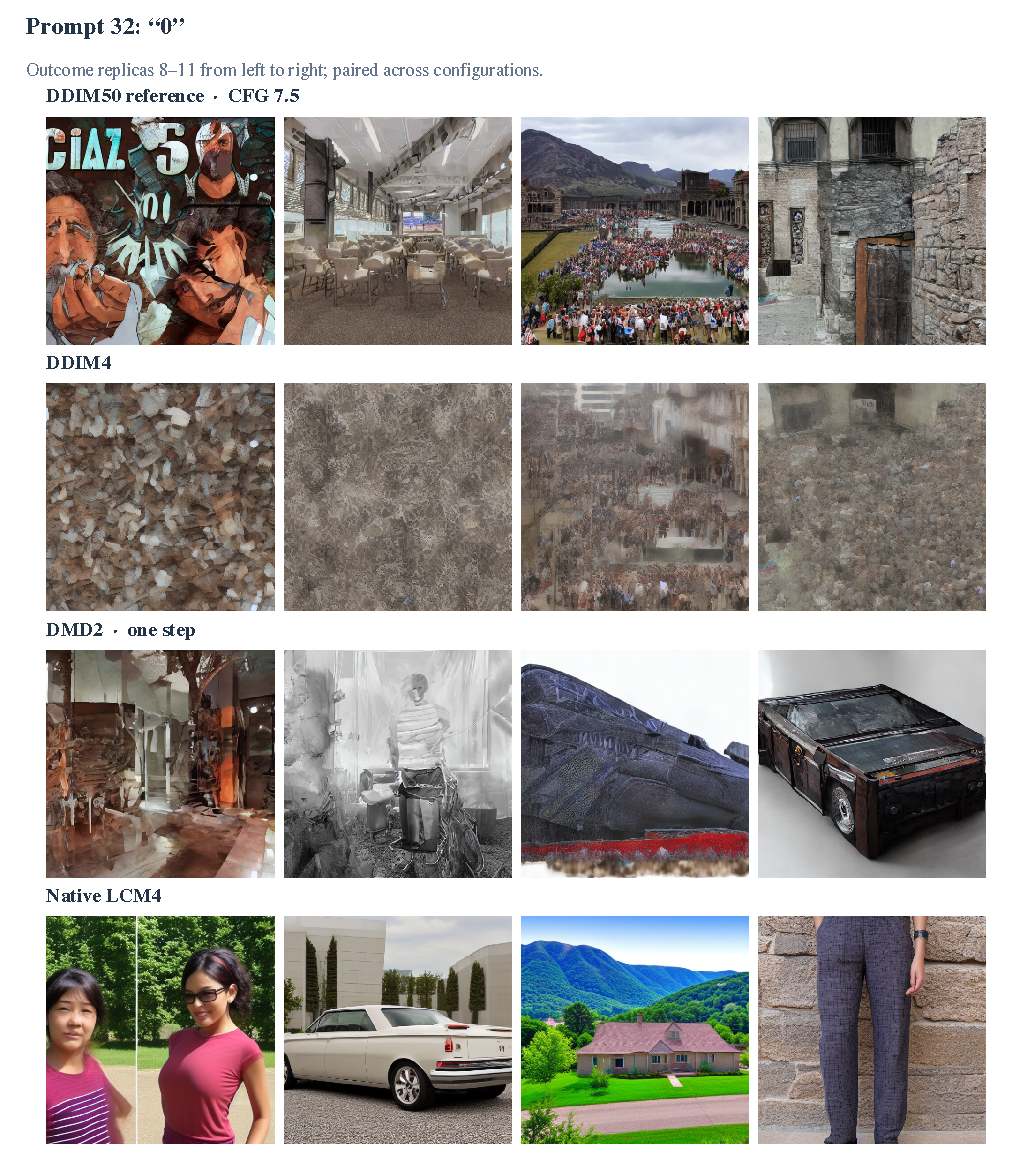
\includegraphics[width=\textwidth]{../figures/t2i_multiseed_0032.pdf}
\caption{Predetermined multi-seed comparison for prompt 32 (``0'').
The three displayed prompts are the smallest held-out original prompt IDs;
columns are outcome replicas 8--11, paired across configurations. The index
rule was recorded before opening images for this display. Every image is
retained without ranking, replacement, or cropping. These abstract prompts
illustrate variation and do not establish semantic coverage.}
\label{fig:t2i_multiseed_32}
\end{figure*}

\begin{figure*}[tp]
\centering
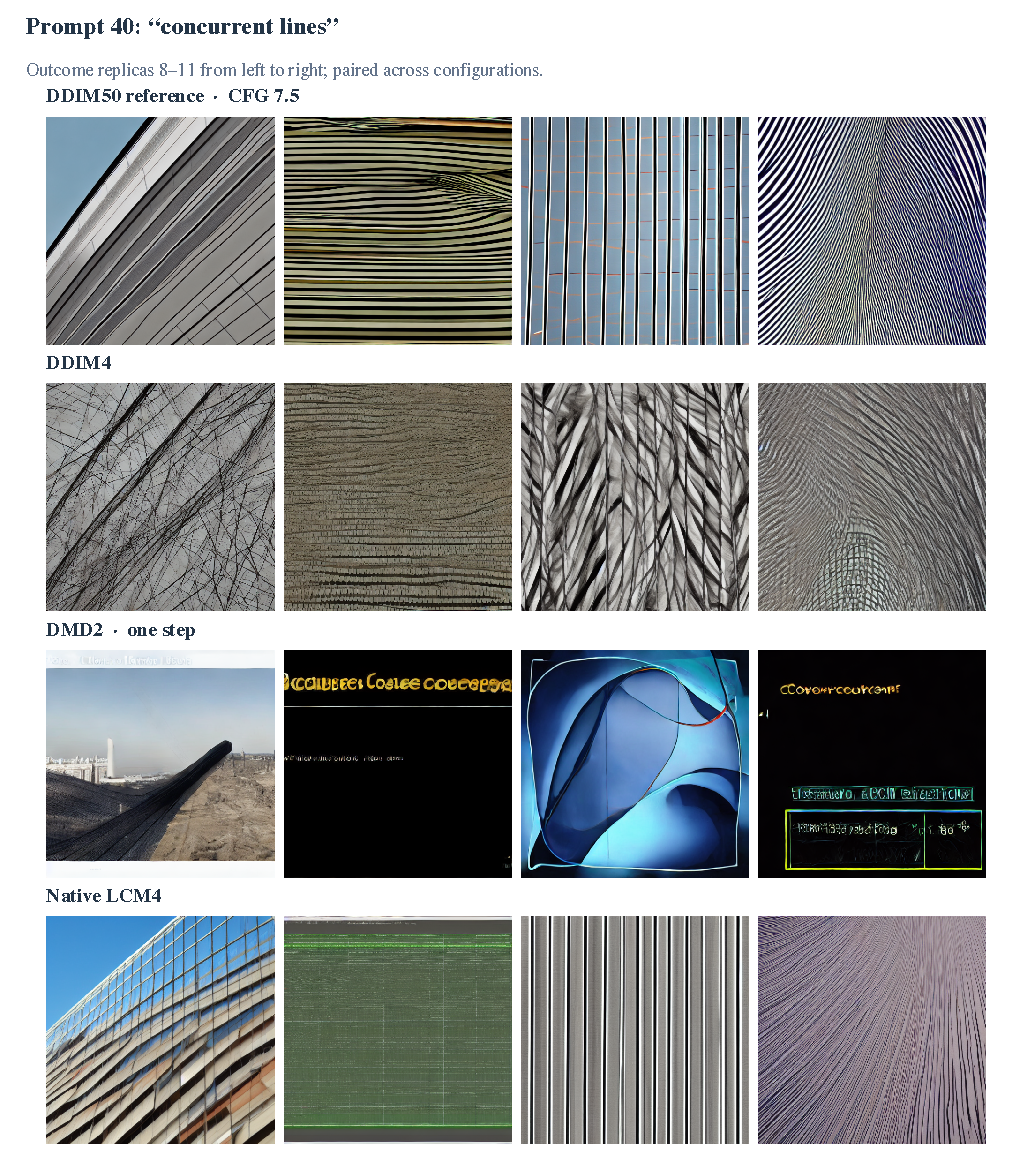
\includegraphics[width=\textwidth]{../figures/t2i_multiseed_0040.pdf}
\caption{Predetermined multi-seed comparison for prompt 40 (``concurrent lines'').
The three displayed prompts are the smallest held-out original prompt IDs;
columns are outcome replicas 8--11, paired across configurations. The index
rule was recorded before opening images for this display. Every image is
retained without ranking, replacement, or cropping. These abstract prompts
illustrate variation and do not establish semantic coverage.}
\label{fig:t2i_multiseed_40}
\end{figure*}

\begin{figure*}[tp]
\centering
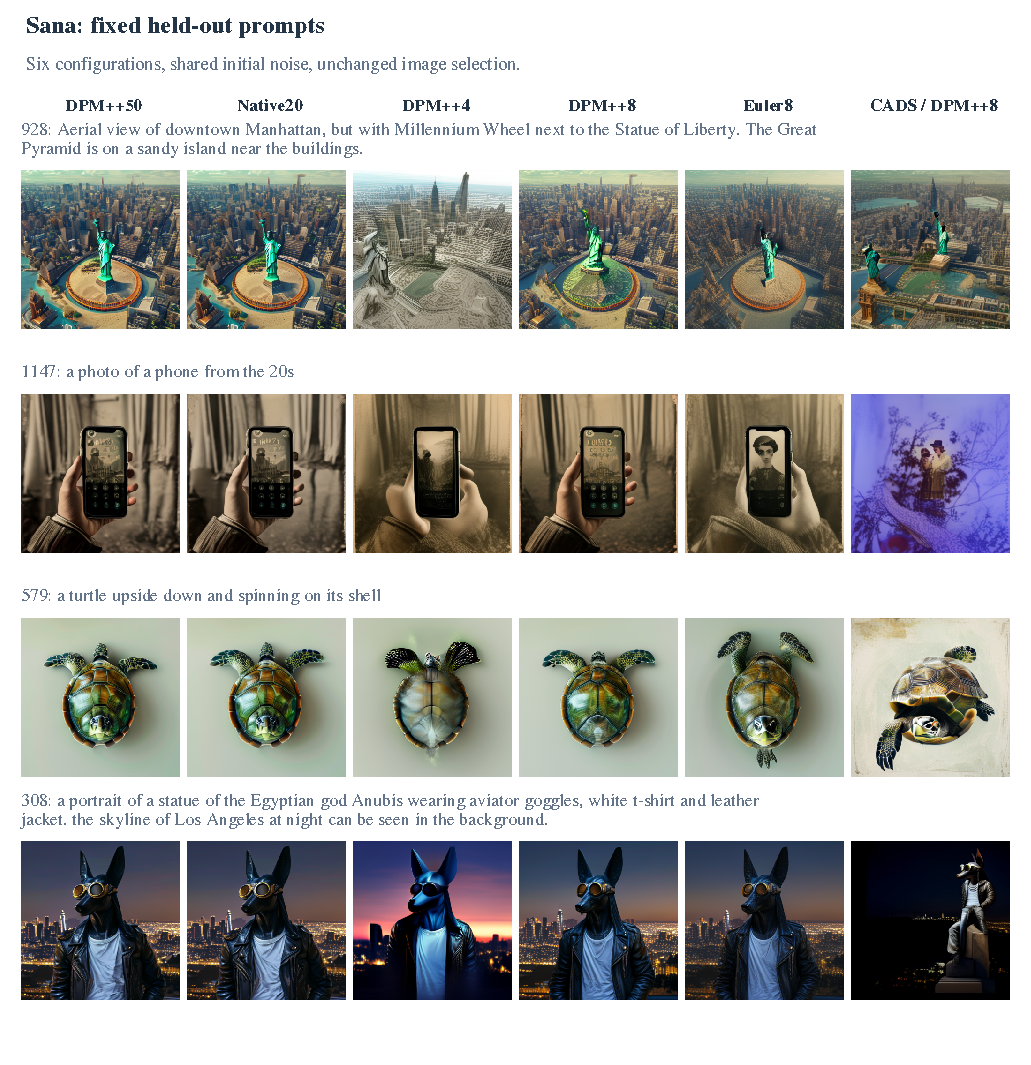
\includegraphics[width=\textwidth]{../figures/t2i_flow_qualitative.pdf}
\caption{Predetermined Sana comparison. Rows are the first four prompts in the
frozen shuffled evaluation order, using outcome replica 8. Columns share
initial noise. The 50-step reference and native20 setting are retained;
all seven configurations, including Euler4, remain in the numerical tables.
Images are neither ranked nor replaced.}
\label{fig:flow_qualitative}
\end{figure*}

\appendixbreak
\section{Frozen intervention-policy protocol}
\label{supp:policy_protocol}
We turn the audit into a frozen prompt-level decision rule and evaluate the
selected configurations on new samples. For each of 128 held-out prompts,
eight diagnosis seeds compare two numerical candidates with the reference.
A candidate is eligible when mean predicted preference is at least 0.475,
CLIP alignment loss is at most 0.01, DINO and CLIP spread ratios are at least
0.9, DINO coverage is at least 0.8, and both support-tail excesses are at most
0.05. Among eligible candidates, the rule chooses higher DINO coverage, then
higher preference, then a fixed solver order. It otherwise uses the frozen
higher-budget fallback. These small-sample point criteria select an action;
independent outcomes determine whether that action is adequate.

The SD1.5 shortlist is DPM++8/UniPC8 with DPM++16 fallback. The flow transfer
uses DPM++8/Euler8 with native20 fallback and exactly the same numerical
thresholds. Reference fit and calibration are model-specific. Sixteen separate
outcome seeds per prompt evaluate each policy. An approximate fixed-policy intersection--union
test\cite{berger1996intersection} requires all one-sided 95\% prompt-bootstrap constraints to pass:
preference at least 0.45, alignment loss at most 0.01, both spread ratios at
least 0.9, and both support excesses at most 0.05. The fallback receives the
same evaluation. All-arm intervals are descriptive; four prespecified paired
policy contrasts use Bonferroni intervals within each study. The original
coverage criterion uses shared initial-noise seeds. The secondary
independent-noise sensitivity specified after outcome access below evaluates the same saved decisions with
disjoint outcome halves; it does not retrospectively change eligibility or gates.

The comparators include fixed strong solvers, preference-and-alignment selection,
quality-constrained Vendi, Vendi alone, PRDC harmonic selection, a random
shortlist of the same size, and exhaustive search over the declared eight-step
candidate pool. The full matrix is generated for fair comparison, while policy
costs count only the candidates observed by that policy. A two-candidate audit
requires $8(50+8+8)=528$ denoiser calls per prompt before outcome generation,
plus feature extraction and scoring. Fixed solvers have no online diagnostic
cost. We report inference savings and their amortization separately from
this overhead.
Preparing the support audit also generates $(32\times16+256)\times50=38{,}400$
reference calls per family for its named policy reference. This reusable
fitting/calibration pool is separate from per-prompt diagnosis. Charging it
across the 128 evaluation prompts adds 300 calls per prompt: the lower-bound
cold-start break-even is then 428 outputs for SD1.5 and 145 for Sana, rather
than the prepared-audit bounds of 273 and 93. All bounds exclude feature and
reward computation. Additional reference pools, development runs, and the full
comparison matrix belong to the research cost ledger rather than a claim of
realized deployment savings.
An additional prespecified assignment control randomly permutes the audit's
selected actions across prompts, preserving their exact counts and inference
cost. It tests prompt-specific assignment using independent outcome preference
and the fraction of prompts whose observed 16-seed preference falls below 0.4.
This secondary replay receives the same diagnostic cost; its conditional
bootstrap intervals are approximate because the permutation couples prompts.
\section{Complete intervention-policy outcomes}
\label{supp:policy_outcomes}
Every frozen policy is evaluated with outcome replicas 8--23. Coverage in
the original tables compares coupled initial-noise samples; the independent-
noise sensitivity below keeps cardinality fixed and reports its different
estimand separately. The four primary contrasts retain their original within-study multiplicity adjustment. The two secondary assignment contrasts are a separate family. No policy is chosen from these outcomes.
\paragraph{SD1.5.}
The original policy reaches learned preference 0.482 at 14.06 calls per image.
The complete absolute outcomes and adjusted contrasts are reported below.
\begin{table*}[t]\centering\small
\caption{All SD1.5 policies. Spread ratios are ratios of mean within-prompt variances. Intervals for all policies are descriptive; only the frozen audit receives the primary intersection--union interpretation. Inc.: inconclusive.}
\begin{tabular}{lcccccc}\toprule
Policy & Calls & $\psi$ & DINO spread & CLIP spread & Paired cov. & Gate \\\midrule
Audit & 14.06 & 0.482 [0.477, 0.488] & 1.000 [0.988, 1.010] & 1.003 [0.987, 1.019] & 0.979 & pass \\
Preference + alignment & 12.62 & 0.477 [0.472, 0.483] & 1.008 [0.994, 1.021] & 1.012 [0.995, 1.030] & 0.970 & pass \\
Quality + Vendi & 12.62 & 0.477 [0.472, 0.482] & 1.009 [0.996, 1.022] & 1.010 [0.993, 1.029] & 0.968 & pass \\
Vendi only & 8.00 & 0.444 [0.436, 0.452] & 1.022 [1.005, 1.039] & 1.038 [1.017, 1.061] & 0.945 & inc. \\
PRDC harmonic & 8.00 & 0.447 [0.439, 0.455] & 1.017 [1.001, 1.034] & 1.029 [1.008, 1.052] & 0.944 & inc. \\
Random shortlist & 15.25 & 0.487 [0.482, 0.492] & 1.001 [0.987, 1.017] & 1.015 [0.998, 1.034] & 0.984 & pass \\
Exhaustive & 13.38 & 0.482 [0.477, 0.488] & 1.007 [0.994, 1.019] & 1.002 [0.984, 1.020] & 0.968 & pass \\
Fixed DPM++8 & 8.00 & 0.448 [0.440, 0.456] & 1.014 [0.998, 1.032] & 1.031 [1.011, 1.054] & 0.949 & inc. \\
Fixed UniPC8 & 8.00 & 0.440 [0.432, 0.448] & 1.027 [1.011, 1.045] & 1.037 [1.016, 1.061] & 0.939 & fail \\
Fixed DPM++16 & 16.00 & 0.490 [0.485, 0.494] & 0.994 [0.983, 1.005] & 1.010 [0.996, 1.025] & 0.990 & pass \\
Fixed UniPC16 & 16.00 & 0.488 [0.483, 0.493] & 1.004 [0.992, 1.016] & 1.021 [1.006, 1.036] & 0.987 & pass \\
Shuffled audit & 14.06 & 0.476 [0.469, 0.483] & 1.005 [0.992, 1.018] & 1.021 [1.005, 1.038] & 0.975 & pass \\
\bottomrule\end{tabular}\end{table*}
\begin{table}[t]\centering\small
\caption{SD1.5 audit-minus-baseline contrasts. Intervals are Bonferroni-adjusted within the four primary or two secondary comparisons. Assignment-control inference is approximate conditional on the realized permutation.}
\begin{tabular}{p{.52\columnwidth}r}\toprule
Contrast & Difference [interval] \\\midrule
Preference vs. DPM++8 & 0.034 [0.025, 0.044] \\
Calls vs. DPM++16 & -1.938 [-2.688, -1.250] \\
Calls vs. random shortlist & -1.188 [-1.938, -0.500] \\
Coverage vs. quality + Vendi & 0.011 [0.003, 0.021] \\
\midrule
Preference vs. shuffled audit & 0.007 [-0.001, 0.014] \\
Low-preference rate vs. shuffled audit & -0.039 [-0.094, 0.008] \\
\bottomrule\end{tabular}\end{table}
\paragraph{Sana.}
The unchanged decision rule reaches learned preference 0.502 at 14.28 calls
per image. Its stronger 20-call fallback remains an explicit comparator.
\begin{table*}[t]\centering\small
\caption{All Sana policies. Spread ratios are ratios of mean within-prompt variances. Intervals for all policies are descriptive; only the frozen audit receives the primary intersection--union interpretation. Inc.: inconclusive.}
\begin{tabular}{lcccccc}\toprule
Policy & Calls & $\psi$ & DINO spread & CLIP spread & Paired cov. & Gate \\\midrule
Audit & 14.28 & 0.502 [0.498, 0.506] & 1.043 [1.022, 1.066] & 1.076 [1.047, 1.107] & 0.950 & pass \\
Preference + alignment & 11.94 & 0.505 [0.500, 0.510] & 1.053 [1.028, 1.080] & 1.074 [1.040, 1.113] & 0.910 & pass \\
Quality + Vendi & 11.94 & 0.504 [0.499, 0.509] & 1.060 [1.034, 1.088] & 1.083 [1.048, 1.122] & 0.903 & pass \\
Vendi only & 8.00 & 0.478 [0.470, 0.486] & 1.140 [1.102, 1.181] & 1.158 [1.110, 1.210] & 0.812 & pass \\
PRDC harmonic & 8.00 & 0.480 [0.472, 0.488] & 1.127 [1.093, 1.166] & 1.159 [1.119, 1.204] & 0.876 & pass \\
Random shortlist & 14.84 & 0.503 [0.499, 0.507] & 1.040 [1.020, 1.063] & 1.072 [1.042, 1.106] & 0.953 & pass \\
Exhaustive & 14.28 & 0.502 [0.498, 0.506] & 1.043 [1.022, 1.066] & 1.076 [1.047, 1.107] & 0.950 & pass \\
Fixed DPM++8 & 8.00 & 0.479 [0.471, 0.487] & 1.134 [1.097, 1.174] & 1.164 [1.123, 1.209] & 0.882 & pass \\
Fixed Euler8 & 8.00 & 0.475 [0.466, 0.484] & 1.118 [1.080, 1.158] & 1.146 [1.097, 1.203] & 0.761 & pass \\
Fixed native20 & 20.00 & 0.510 [0.508, 0.513] & 1.001 [0.992, 1.010] & 1.018 [1.002, 1.034] & 0.998 & pass \\
Shuffled audit & 14.28 & 0.495 [0.488, 0.502] & 1.060 [1.031, 1.092] & 1.091 [1.058, 1.128] & 0.939 & pass \\
\bottomrule\end{tabular}\end{table*}
\begin{table}[t]\centering\small
\caption{Sana audit-minus-baseline contrasts. Intervals are Bonferroni-adjusted within the four primary or two secondary comparisons. Assignment-control inference is approximate conditional on the realized permutation.}
\begin{tabular}{p{.52\columnwidth}r}\toprule
Contrast & Difference [interval] \\\midrule
Preference vs. DPM++8 & 0.023 [0.013, 0.034] \\
Calls vs. native20 & -5.719 [-7.031, -4.312] \\
Calls vs. random shortlist & -0.562 [-1.219, -0.094] \\
Coverage vs. quality + Vendi & 0.047 [0.018, 0.081] \\
\midrule
Preference vs. shuffled audit & 0.007 [-0.002, 0.017] \\
Low-preference rate vs. shuffled audit & -0.047 [-0.102, 0.000] \\
\bottomrule\end{tabular}\end{table}

\begin{table*}[t]
\centering
\small
\setlength{\tabcolsep}{3.4pt}
\caption{Operating points of unchanged policies. Absolute outcomes
show saved descriptive 95\% paired prompt-bootstrap intervals over 128
prompts. Preference excludes shared-noise pairs; DINO coverage uses disjoint
eight-sample halves, averaged in both directions. The contrast block uses
99.5\% preference intervals (ten comparisons) and 99.375\% coverage intervals
(eight comparisons). These sensitivities were specified after access to
original outcomes. Inference calls exclude 528 diagnosis calls/prompt and
reusable preparation; fallbacks are SD DPM++16 and Sana native20.}
\label{tab:policy}
\begin{tabular*}{\textwidth}{@{\extracolsep{\fill}}llrrrrr@{}}
\toprule
& & & \multicolumn{2}{c}{Learned preference $\uparrow$}
    & \multicolumn{2}{c@{}}{DINO coverage $\uparrow$} \\
\cmidrule(lr){4-5}\cmidrule(l){6-7}
Model & Policy or comparator & Calls/image & Estimate & Interval & Estimate & Interval \\
\midrule
\multicolumn{7}{@{}l}{\textit{Absolute outcomes}} \\
SD1.5 & \textbf{Audit} & $14.06$ & $0.484$ & $[0.479,\,0.489]$ & $0.913$ & $[0.897,\,0.928]$ \\
 & Quality + Vendi & $12.62$ & $0.479$ & $[0.474,\,0.484]$ & $0.902$ & $[0.883,\,0.920]$ \\
 & Same-count shuffle & $14.06$ & $0.478$ & $[0.471,\,0.484]$ & $0.912$ & $[0.897,\,0.927]$ \\
 & Fixed DPM++8 & $8.00$ & $0.451$ & $[0.444,\,0.459]$ & $0.895$ & $[0.876,\,0.913]$ \\
 & Fallback (DPM++16) & $16.00$ & $0.491$ & $[0.486,\,0.495]$ & $0.927$ & $[0.914,\,0.940]$ \\
\addlinespace[2pt]
Sana & \textbf{Audit} & $14.28$ & $0.502$ & $[0.498,\,0.506]$ & $0.840$ & $[0.810,\,0.867]$ \\
 & Quality + Vendi & $11.94$ & $0.503$ & $[0.498,\,0.508]$ & $0.789$ & $[0.750,\,0.825]$ \\
 & Same-count shuffle & $14.28$ & $0.495$ & $[0.488,\,0.502]$ & $0.844$ & $[0.816,\,0.870]$ \\
 & Fixed DPM++8 & $8.00$ & $0.480$ & $[0.472,\,0.487]$ & $0.775$ & $[0.743,\,0.807]$ \\
 & Fallback (native20) & $20.00$ & $0.510$ & $[0.507,\,0.512]$ & $0.906$ & $[0.889,\,0.922]$ \\
\midrule
\multicolumn{7}{@{}l}{\textit{Audit minus comparator}} \\
SD1.5 & Quality + Vendi & $+1.44$ & $+0.0053$ & $[0.0019,\,0.0097]$ & $+0.0107$ & $[-0.0015,\,0.0269]$ \\
 & Same-count shuffle & $0.00$ & $+0.0063$ & $[-0.0025,\,0.0150]$ & $+0.0010$ & $[-0.0132,\,0.0161]$ \\
Sana & Quality + Vendi & $+2.34$ & $-0.0014$ & $[-0.0057,\,0.0024]$ & $+0.0508$ & $[0.0148,\,0.0947]$ \\
 & Same-count shuffle & $0.00$ & $+0.0068$ & $[-0.0038,\,0.0190]$ & $-0.0039$ & $[-0.0453,\,0.0365]$ \\
\bottomrule
\end{tabular*}
\end{table*}


\subsection{Sensitivity to sampling coupling}
\label{sec:t2i-coupling-sensitivity}
Two secondary sensitivity protocols were specified after access to the original outcome analyses; the original paired-seed results remain the primary record. Neither changes an intervention, routing threshold, candidate pool, or saved decision. Their uncertainty remains approximate prompt-bootstrap inference.

\paragraph{Coverage at fixed cardinality.}
For each of the 128 held-out prompts, divide the 16 outcome seeds into
$A=\{8,\ldots,15\}$ and $B=\{16,\ldots,23\}$.
Write $R_A,R_B$ for the reference samples and $Q_A,Q_B$ for candidate
samples from the two halves. Paired coverage averages $(R_A,Q_A)$ and
$(R_B,Q_B)$, while disjoint coverage averages $(R_A,Q_B)$ and $(R_B,Q_A)$.
Both use eight reference and eight candidate samples and the third-nearest
reference neighbor, preserving cardinality while changing coupling.
We retain all 29 SD1.5 and seven Sana arms, both feature representations,
all four PRDC measurements, and all 23 frozen policies. The bootstrap
resamples whole prompts, preserving dependence between the two directions.
The eight declared DINO-coverage contrasts use 99.375\% percentile
intervals with Bonferroni allocation across both families. The saved
percentile levels are .003125/.996875.

Let $\widehat C$ be the fraction of $n$ reference points whose
$k$-nearest-neighbor ball contains at least one of the $m$ candidate points,
where $1\leq k<n$. For independent reference and candidate draws from the
same continuous distribution with no distance ties, its expectation is
known~\cite[Lemma~2]{naeem2020density}:
\begin{equation}
 \mathbb E[\widehat C]=1-\prod_{\ell=1}^{k}\frac{n-\ell}{m+n-\ell}.
\label{eq:supp_expected_coverage}
\end{equation}
At $n=m=8,k=3$ it is $12/13\approx.9231$, whereas using the identical image set as both inputs gives one. Independent reference-self coverage is .9302 on SD1.5 (descriptive 95\% interval $[.9155,.9443]$) and .9097 on Sana ($[.8911,.9272]$). Thus neither a shortfall from one nor agreement with this finite-sample expectation quantifies missing population support. The observed audit--shuffle disjoint-coverage differences are .0010 on SD1.5 ($[-.0132,.0161]$) and $-.0039$ on Sana ($[-.0453,.0365]$), with the declared adjusted intervals. The SD1.5 audit--quality+Vendi interval includes zero; Sana retains a positive difference at increased cost.

\paragraph{Independent-noise preference.}
Let $a_i,b_i$ be candidate and reference PickScore logits for outcome seed $i$ at one prompt, and let $\sigma$ denote the sigmoid. The original score is $\widehat\psi_{\rm pair}=m^{-1}\sum_i\sigma(a_i-b_i)$, with $m=16$. We additionally compute
\begin{equation}
 \widehat\psi_{\rm ind}=\frac{1}{m(m-1)}\sum_{i\ne j}\sigma(a_i-b_j).
\label{eq:supp_independent_preference}
\end{equation}
This is a symmetrized order-two U-statistic over independent paired seed units and estimates preference between independent draws from the two conditional distributions. Its 240 within-prompt cross-pairs are dependent; only the 128 prompt units are bootstrapped (10,000 repetitions, fixed seed 74117). For the same reference, both estimators equal one half. Original diagonal policy means reproduce exactly. All 94 arm/reference comparisons (SD 29 against three references, Sana 7 against its reference), all 23 frozen policies, and every audit-minus-other-policy contrast are reported in the saved CSV/JSON records. No outcome is used to reroute a prompt.

The ten declared preference contrasts use 99.5\% intervals across both families. Audit independent-minus-paired preference is .00156 on SD1.5 ($[.00075,.00251]$) and $-.00020$ on Sana ($[-.00055,.00020]$). Independent-noise audit--shuffle differences remain unresolved: .00625 ($[-.00251,.01497]$) and .00685 ($[-.00384,.01900]$). Mean raw ImageReward differences are unchanged by pairing, by linearity; no rescoring is needed. These checks identify which conclusions depend on coupling without presenting the exploratory sensitivities as untouched confirmation.



\begin{table*}[tp]
\centering\small
\caption{Complete independent-noise preference sensitivity for all 23 frozen policies. The final-column intervals are descriptive 95\% paired-prompt bootstrap intervals for independent minus paired preference.}
\begin{tabular}{llrrrr}
\toprule Family & Policy & NFE & Paired & Independent & Difference [95\% CI] \\ \midrule
SD1.5 & Audit & 14.06 & 0.4825 & 0.4840 & +0.0016 [0.0010, 0.0022]\\
SD1.5 & Preference + alignment & 12.62 & 0.4774 & 0.4791 & +0.0017 [0.0011, 0.0024]\\
SD1.5 & Quality + Vendi & 12.62 & 0.4769 & 0.4787 & +0.0017 [0.0012, 0.0024]\\
SD1.5 & Vendi only & 8.00 & 0.4441 & 0.4473 & +0.0032 [0.0024, 0.0040]\\
SD1.5 & PRDC harmonic & 8.00 & 0.4469 & 0.4501 & +0.0032 [0.0024, 0.0040]\\
SD1.5 & Random shortlist & 15.25 & 0.4866 & 0.4877 & +0.0011 [0.0006, 0.0017]\\
SD1.5 & Exhaustive & 13.38 & 0.4825 & 0.4840 & +0.0016 [0.0010, 0.0022]\\
SD1.5 & Fixed DPM++8 & 8.00 & 0.4481 & 0.4513 & +0.0032 [0.0024, 0.0040]\\
SD1.5 & Fixed UniPC8 & 8.00 & 0.4403 & 0.4438 & +0.0035 [0.0027, 0.0043]\\
SD1.5 & Fixed DPM++16 & 16.00 & 0.4895 & 0.4906 & +0.0011 [0.0005, 0.0017]\\
SD1.5 & Fixed UniPC16 & 16.00 & 0.4880 & 0.4892 & +0.0011 [0.0005, 0.0018]\\
SD1.5 & Same-count shuffle & 14.06 & 0.4758 & 0.4778 & +0.0020 [0.0013, 0.0027]\\
Sana & Audit & 14.28 & 0.5023 & 0.5021 & -0.0002 [-0.0004, 0.0001]\\
Sana & Preference + alignment & 11.94 & 0.5051 & 0.5047 & -0.0004 [-0.0008, -0.0001]\\
Sana & Quality + Vendi & 11.94 & 0.5039 & 0.5035 & -0.0004 [-0.0007, -0.0001]\\
Sana & Vendi only & 8.00 & 0.4781 & 0.4782 & +0.0001 [-0.0003, 0.0005]\\
Sana & PRDC harmonic & 8.00 & 0.4800 & 0.4802 & +0.0003 [-0.0001, 0.0007]\\
Sana & Random shortlist & 14.84 & 0.5028 & 0.5026 & -0.0002 [-0.0005, 0.0001]\\
Sana & Exhaustive & 14.28 & 0.5023 & 0.5021 & -0.0002 [-0.0004, 0.0001]\\
Sana & Fixed DPM++8 & 8.00 & 0.4794 & 0.4797 & +0.0003 [-0.0001, 0.0007]\\
Sana & Fixed Euler8 & 8.00 & 0.4749 & 0.4750 & +0.0001 [-0.0004, 0.0006]\\
Sana & Fixed native20 & 20.00 & 0.5101 & 0.5097 & -0.0005 [-0.0007, -0.0003]\\
Sana & Same-count shuffle & 14.28 & 0.4954 & 0.4953 & -0.0002 [-0.0005, 0.0002]\\
\bottomrule
\end{tabular}
\end{table*}

\begin{table*}[tp]
\centering\small
\caption{All ten declared independent-noise preference contrasts. Bonferroni percentile intervals are 99.5\% each across the ten-contrast family; all policies remain unchanged.}
\begin{tabular}{llrr}
\toprule Family & Contrast & Difference & Adjusted interval \\ \midrule
SD1.5 & Audit: independent minus paired & +0.0016 & [+0.00075, +0.00251]\\
SD1.5 & Quality+Vendi: independent minus paired & +0.0017 & [+0.00094, +0.00271]\\
SD1.5 & Independent audit minus DPM++8 & +0.0327 & [+0.02320, +0.04206]\\
SD1.5 & Independent audit minus quality+Vendi & +0.0053 & [+0.00185, +0.00975]\\
SD1.5 & Independent audit minus same-count shuffle & +0.0063 & [-0.00251, +0.01497]\\
Sana & Audit: independent minus paired & -0.0002 & [-0.00055, +0.00020]\\
Sana & Quality+Vendi: independent minus paired & -0.0004 & [-0.00089, +0.00004]\\
Sana & Independent audit minus DPM++8 & +0.0225 & [+0.01167, +0.03440]\\
Sana & Independent audit minus quality+Vendi & -0.0014 & [-0.00568, +0.00235]\\
Sana & Independent audit minus same-count shuffle & +0.0068 & [-0.00384, +0.01900]\\
\bottomrule
\end{tabular}
\end{table*}

\begin{table*}[tp]
\centering\small
\caption{All frozen policies under the fixed-cardinality coverage sensitivity. DINO coverage uses eight samples in each set and $k=3$. Shared-seed and disjoint-seed comparisons each average their two outcome halves. Brackets are descriptive 95\% paired-prompt bootstrap intervals.}
\begin{tabular}{llcc}
\toprule Family & Policy & Shared-seed coverage & Disjoint-seed coverage \\ \midrule
SD1.5 & Audit & 0.991 [0.986, 0.995] & 0.913 [0.897, 0.928]\\
SD1.5 & Preference + alignment & 0.992 [0.988, 0.996] & 0.903 [0.885, 0.921]\\
SD1.5 & Quality + Vendi & 0.991 [0.986, 0.995] & 0.902 [0.883, 0.920]\\
SD1.5 & Vendi only & 0.975 [0.966, 0.982] & 0.882 [0.858, 0.903]\\
SD1.5 & PRDC harmonic & 0.974 [0.966, 0.981] & 0.888 [0.869, 0.906]\\
SD1.5 & Random shortlist & 0.993 [0.986, 0.998] & 0.921 [0.906, 0.936]\\
SD1.5 & Exhaustive & 0.985 [0.978, 0.991] & 0.908 [0.891, 0.925]\\
SD1.5 & Fixed DPM++8 & 0.983 [0.977, 0.989] & 0.895 [0.876, 0.913]\\
SD1.5 & Fixed UniPC8 & 0.970 [0.961, 0.978] & 0.866 [0.841, 0.889]\\
SD1.5 & Fixed DPM++16 & 0.997 [0.995, 0.999] & 0.927 [0.914, 0.940]\\
SD1.5 & Fixed UniPC16 & 0.996 [0.993, 0.999] & 0.914 [0.897, 0.930]\\
SD1.5 & Same-count shuffle & 0.991 [0.986, 0.995] & 0.912 [0.897, 0.927]\\
Sana & Audit & 0.968 [0.955, 0.979] & 0.840 [0.810, 0.867]\\
Sana & Preference + alignment & 0.938 [0.915, 0.958] & 0.787 [0.750, 0.820]\\
Sana & Quality + Vendi & 0.930 [0.902, 0.954] & 0.789 [0.750, 0.825]\\
Sana & Vendi only & 0.870 [0.836, 0.901] & 0.708 [0.667, 0.746]\\
Sana & PRDC harmonic & 0.928 [0.906, 0.946] & 0.772 [0.738, 0.805]\\
Sana & Random shortlist & 0.971 [0.958, 0.982] & 0.837 [0.806, 0.866]\\
Sana & Exhaustive & 0.968 [0.955, 0.979] & 0.840 [0.810, 0.867]\\
Sana & Fixed DPM++8 & 0.934 [0.917, 0.950] & 0.775 [0.743, 0.807]\\
Sana & Fixed Euler8 & 0.837 [0.800, 0.871] & 0.666 [0.624, 0.705]\\
Sana & Fixed native20 & 0.999 [0.998, 1.000] & 0.906 [0.889, 0.922]\\
Sana & Same-count shuffle & 0.964 [0.951, 0.977] & 0.844 [0.816, 0.870]\\
\bottomrule\end{tabular}
\end{table*}
\begin{table*}[tp]
\centering\small
\caption{All eight declared coverage sensitivity contrasts. Percentile intervals are 99.375\% each across the eight-comparison family. These secondary sensitivities were specified after access to earlier outcomes and evaluate unchanged policy decisions.}
\begin{tabular}{llc}
\toprule Family & Contrast & Difference [adjusted interval] \\ \midrule
SD1.5 & Audit: disjoint minus shared seeds & -0.0776 [-0.0991, -0.0571]\\
SD1.5 & Quality + Vendi: disjoint minus shared seeds & -0.0884 [-0.1143, -0.0649]\\
SD1.5 & Disjoint audit minus quality + Vendi & +0.0107 [-0.0015, +0.0269]\\
SD1.5 & Disjoint audit minus same-count shuffle & +0.0010 [-0.0132, +0.0161]\\
Sana & Audit: disjoint minus shared seeds & -0.1279 [-0.1610, -0.0973]\\
Sana & Quality + Vendi: disjoint minus shared seeds & -0.1406 [-0.1742, -0.1089]\\
Sana & Disjoint audit minus quality + Vendi & +0.0508 [+0.0148, +0.0947]\\
Sana & Disjoint audit minus same-count shuffle & -0.0039 [-0.0453, +0.0365]\\
\bottomrule\end{tabular}
\end{table*}


\section{Independent reward-model sensitivity}
\label{supp:imagereward}
ImageReward-v1.0\cite{xu2023imagereward} was prespecified as a secondary outcome-only check before analyzing held-out text-to-image outcomes. Its BLIP-based reward was never used to develop or select the audit policies. Scores use the official FP32 model, normalization and preprocessing; batched and official scalar-loop scores agreed within $9.3\times10^{-7}$. Both ImageReward and PickScore are learned proxies rather than a human evaluation. All arms and policies are retained below. Mean scalar rewards are unchanged
by the pairing used for cross-method comparisons; the paired win fractions
retain their stated coupled-sample interpretation.
For each of 128 held-out prompts, we average the 16 separate outcome replicas. Descriptive 95\% intervals resample prompts jointly across arms. The four prespecified audit-minus-fixed/fallback scalar-reward contrasts across the two model families use 98.75\% Bonferroni intervals. Pairwise win fractions are descriptive, with ties counted as one half; normalized scalar differences are not human preference probabilities.
\begin{table*}[t]\centering\small
\caption{SD1.5 ImageReward arms. All comparisons use the common declared reference. Win is the fraction of paired images with higher predicted reward; brackets are descriptive 95\% prompt-bootstrap intervals.}
\begin{tabular}{lccc}\toprule
Configuration & Reward & Difference from reference & Paired win \\\midrule
DDIM50 (CFG7.5) & 0.210 [0.065, 0.350] & 0.000 [0.000, 0.000] & 0.500 [0.500, 0.500] \\
DDIM4 & -1.091 [-1.205, -0.974] & -1.301 [-1.425, -1.177] & 0.111 [0.089, 0.135] \\
DDIM8 & -0.146 [-0.285, -0.009] & -0.356 [-0.414, -0.297] & 0.298 [0.269, 0.329] \\
Trailing DDIM4 & -0.392 [-0.527, -0.257] & -0.602 [-0.682, -0.522] & 0.209 [0.179, 0.240] \\
Trailing DDIM8 & 0.072 [-0.072, 0.216] & -0.138 [-0.174, -0.101] & 0.350 [0.325, 0.376] \\
Stochastic DDIM4 & -1.393 [-1.493, -1.288] & -1.603 [-1.727, -1.478] & 0.061 [0.046, 0.078] \\
Stochastic DDIM8 & -0.221 [-0.362, -0.083] & -0.431 [-0.491, -0.371] & 0.275 [0.247, 0.305] \\
DDIM4 (CFG3) & -1.534 [-1.630, -1.435] & -1.744 [-1.872, -1.614] & 0.051 [0.036, 0.070] \\
DDIM8 (CFG3) & -0.645 [-0.776, -0.512] & -0.855 [-0.948, -0.761] & 0.168 [0.141, 0.198] \\
DPM++4 & -0.342 [-0.475, -0.211] & -0.552 [-0.625, -0.480] & 0.211 [0.185, 0.240] \\
DPM++8 & 0.109 [-0.039, 0.257] & -0.101 [-0.133, -0.069] & 0.383 [0.361, 0.406] \\
UniPC4 & -0.340 [-0.472, -0.211] & -0.550 [-0.621, -0.481] & 0.221 [0.194, 0.250] \\
UniPC8 & 0.105 [-0.040, 0.250] & -0.104 [-0.136, -0.072] & 0.376 [0.354, 0.399] \\
CADS--DDIM4 & -1.238 [-1.349, -1.120] & -1.447 [-1.576, -1.321] & 0.099 [0.079, 0.120] \\
CADS--DDIM8 & -0.593 [-0.723, -0.459] & -0.803 [-0.906, -0.703] & 0.206 [0.176, 0.236] \\
CADS--DPM++4 & -1.061 [-1.165, -0.954] & -1.271 [-1.386, -1.157] & 0.118 [0.096, 0.142] \\
CADS--DPM++8 & -0.607 [-0.726, -0.484] & -0.817 [-0.910, -0.726] & 0.213 [0.187, 0.239] \\
DDIM50 (CFG1.75) & -0.576 [-0.704, -0.450] & -0.786 [-0.860, -0.710] & 0.173 [0.150, 0.198] \\
DDIM50 (CFG1) & -1.250 [-1.345, -1.154] & -1.460 [-1.566, -1.351] & 0.084 [0.066, 0.105] \\
LCM4 & -0.169 [-0.331, -0.007] & -0.378 [-0.453, -0.306] & 0.324 [0.292, 0.356] \\
LCM8 & -0.247 [-0.409, -0.081] & -0.456 [-0.543, -0.372] & 0.328 [0.294, 0.362] \\
Hybrid LCM4 & -0.273 [-0.424, -0.121] & -0.483 [-0.558, -0.413] & 0.312 [0.287, 0.339] \\
Hybrid LCM8 & -0.197 [-0.354, -0.037] & -0.406 [-0.491, -0.328] & 0.347 [0.315, 0.378] \\
DMD2 & -0.193 [-0.327, -0.057] & -0.403 [-0.481, -0.326] & 0.332 [0.302, 0.362] \\
DPM++16 & 0.193 [0.047, 0.337] & -0.017 [-0.041, 0.006] & 0.464 [0.440, 0.487] \\
UniPC16 & 0.179 [0.032, 0.325] & -0.031 [-0.054, -0.007] & 0.451 [0.426, 0.477] \\
Trailing DDIM16 & 0.190 [0.043, 0.338] & -0.019 [-0.044, 0.006] & 0.443 [0.420, 0.465] \\
CADS--DPM++16 & -0.241 [-0.378, -0.105] & -0.451 [-0.525, -0.378] & 0.316 [0.288, 0.346] \\
Tuned CADS--DPM++8 & -0.101 [-0.235, 0.032] & -0.311 [-0.356, -0.265] & 0.323 [0.298, 0.349] \\
\bottomrule\end{tabular}\end{table*}
\begin{table*}[t]\centering\small
\caption{SD1.5 ImageReward policies. All comparisons use the common declared reference. Win is the fraction of paired images with higher predicted reward; brackets are descriptive 95\% prompt-bootstrap intervals.}
\begin{tabular}{lccc}\toprule
Configuration & Reward & Difference from reference & Paired win \\\midrule
Audit & 0.184 [0.038, 0.329] & -0.026 [-0.051, -0.001] & 0.444 [0.421, 0.468] \\
Preference + alignment & 0.163 [0.016, 0.308] & -0.047 [-0.074, -0.019] & 0.428 [0.404, 0.452] \\
Quality + Vendi & 0.162 [0.015, 0.307] & -0.048 [-0.075, -0.021] & 0.427 [0.403, 0.451] \\
Vendi only & 0.111 [-0.035, 0.256] & -0.099 [-0.131, -0.066] & 0.382 [0.359, 0.405] \\
PRDC harmonic & 0.113 [-0.034, 0.260] & -0.097 [-0.128, -0.065] & 0.380 [0.357, 0.402] \\
Random shortlist & 0.188 [0.044, 0.332] & -0.022 [-0.046, 0.003] & 0.459 [0.437, 0.482] \\
Exhaustive & 0.163 [0.015, 0.312] & -0.047 [-0.077, -0.018] & 0.437 [0.414, 0.460] \\
Fixed DPM++8 & 0.109 [-0.039, 0.257] & -0.101 [-0.133, -0.069] & 0.383 [0.361, 0.406] \\
Fixed UniPC8 & 0.105 [-0.040, 0.250] & -0.104 [-0.136, -0.072] & 0.376 [0.354, 0.399] \\
Fixed DPM++16 & 0.193 [0.047, 0.337] & -0.017 [-0.041, 0.006] & 0.464 [0.440, 0.487] \\
Fixed UniPC16 & 0.179 [0.032, 0.325] & -0.031 [-0.054, -0.007] & 0.451 [0.426, 0.477] \\
Same-count shuffle & 0.169 [0.021, 0.317] & -0.041 [-0.069, -0.014] & 0.437 [0.411, 0.463] \\
\bottomrule\end{tabular}\end{table*}
\begin{table*}[t]\centering\small
\caption{Sana ImageReward arms. All comparisons use the common declared reference. Win is the fraction of paired images with higher predicted reward; brackets are descriptive 95\% prompt-bootstrap intervals.}
\begin{tabular}{lccc}\toprule
Configuration & Reward & Difference from reference & Paired win \\\midrule
Flow-DPM++50 & 1.225 [1.103, 1.342] & 0.000 [0.000, 0.000] & 0.500 [0.500, 0.500] \\
Flow-DPM++20 & 1.225 [1.104, 1.342] & 0.001 [-0.007, 0.009] & 0.473 [0.449, 0.497] \\
DPM++4 & 0.607 [0.469, 0.741] & -0.618 [-0.719, -0.522] & 0.176 [0.144, 0.209] \\
DPM++8 & 1.154 [1.032, 1.270] & -0.071 [-0.096, -0.048] & 0.406 [0.377, 0.435] \\
Euler4 & 0.063 [-0.099, 0.225] & -1.162 [-1.314, -1.014] & 0.110 [0.081, 0.143] \\
Euler8 & 1.121 [0.997, 1.241] & -0.103 [-0.137, -0.073] & 0.361 [0.330, 0.392] \\
CADS--DPM++8 & 0.672 [0.542, 0.801] & -0.553 [-0.621, -0.488] & 0.194 [0.170, 0.220] \\
\bottomrule\end{tabular}\end{table*}
\begin{table*}[t]\centering\small
\caption{Sana ImageReward policies. All comparisons use the common declared reference. Win is the fraction of paired images with higher predicted reward; brackets are descriptive 95\% prompt-bootstrap intervals.}
\begin{tabular}{lccc}\toprule
Configuration & Reward & Difference from reference & Paired win \\\midrule
Audit & 1.199 [1.077, 1.316] & -0.025 [-0.042, -0.010] & 0.448 [0.420, 0.476] \\
Preference + alignment & 1.193 [1.073, 1.308] & -0.032 [-0.051, -0.013] & 0.435 [0.407, 0.463] \\
Quality + Vendi & 1.189 [1.066, 1.307] & -0.035 [-0.054, -0.018] & 0.437 [0.409, 0.466] \\
Vendi only & 1.136 [1.011, 1.256] & -0.089 [-0.115, -0.064] & 0.384 [0.356, 0.415] \\
PRDC harmonic & 1.151 [1.029, 1.268] & -0.074 [-0.098, -0.051] & 0.393 [0.364, 0.421] \\
Random shortlist & 1.201 [1.078, 1.316] & -0.024 [-0.040, -0.009] & 0.447 [0.419, 0.474] \\
Exhaustive & 1.199 [1.077, 1.316] & -0.025 [-0.042, -0.010] & 0.448 [0.420, 0.476] \\
Fixed DPM++8 & 1.154 [1.032, 1.270] & -0.071 [-0.096, -0.048] & 0.406 [0.377, 0.435] \\
Fixed Euler8 & 1.121 [0.997, 1.241] & -0.103 [-0.137, -0.073] & 0.361 [0.330, 0.392] \\
Fixed native20 & 1.225 [1.104, 1.342] & 0.001 [-0.007, 0.009] & 0.473 [0.449, 0.497] \\
Same-count shuffle & 1.194 [1.072, 1.309] & -0.031 [-0.049, -0.013] & 0.469 [0.443, 0.496] \\
\bottomrule\end{tabular}\end{table*}
\begin{table*}[t]\centering\small
\caption{Secondary cross-family ImageReward contrasts. Four jointly Bonferroni-adjusted comparisons; no policy or quality gate was changed using these outcomes.}
\begin{tabular}{llc}\toprule
Model & Audit minus baseline & Scalar reward difference [98.75\% interval] \\\midrule
SD1.5 & Fixed DPM++8 & 0.075 [0.044, 0.107] \\
SD1.5 & Fixed DPM++16 & -0.009 [-0.029, 0.009] \\
Sana & Fixed DPM++8 & 0.046 [0.022, 0.072] \\
Sana & Fixed native20 & -0.026 [-0.046, -0.009] \\
\bottomrule\end{tabular}\end{table*}
LCM4 and LCM8 improve scalar ImageReward relative to the CFG1 sensitivity
reference by 1.081 [0.962, 1.205] and 1.004 [0.879, 1.132], respectively.
DMD2 improves relative to its matched CFG1.75 teacher by 0.383 [0.309, 0.460].

\paragraph{Agreements and quality tradeoffs.}
ImageReward corroborates the primary policies' gains over fixed DPM++8:
the mean normalized reward increases by 0.0748 [0.0435,0.1065] on SD1.5
and 0.0458 [0.0221,0.0722] on Sana, using the four-comparison adjustment.
The audit-minus-fallback difference is unresolved on SD1.5,
$-0.0089$ [$-0.0293,0.0091$], but negative on Sana,
$-0.0261$ [$-0.0461,-0.0093$]. Thus reduced inference cost has a measurable
quality tradeoff relative to Sana's strong 20-call fallback, even though the
prespecified PickScore-based acceptance margin passes. No ImageReward
noninferiority margin was prespecified, and passing the earlier gates does
not establish reward equivalence. Descriptive differences from the 50-call
common references are also negative for both selected policies.

The reference dependence of native DMD2 persists under this second reward
model. Its scalar reward difference is $+0.3826$ [0.3088,0.4602] against
the matched CFG1.75 teacher and $-0.4032$ [$-0.4808,-0.3257$] against
CFG7.5. These descriptive 95\% intervals accompany all native-reference
sensitivities above. Both learned reward models therefore support the
matched-reference quality improvement while the image-feature and latent
spread changes have opposing directions. These agreements validate the
stated proxy measurements; neither model substitutes for a human study.

\appendixbreak
\twocolumn[{\section{Reproducibility: display names and artifact identifiers}
\label{supp:identifiers}
Tables use readable method names. The mapping below preserves the identifiers
in the immutable result records; $K$ denotes the recorded step/call suffix,
with CAS ceilings interpreted as specified in Sec.~\ref{supp:cifar}.
The accompanying identifier CSV lists each relabeled reward-table entry.
Model revisions, exact sampling configurations, seed streams, and complete
resource ledgers remain in the study sections and source manifests.

\begin{minipage}{\textwidth}
\centering\footnotesize
\captionsetup{hypcap=false}
\setlength{\tabcolsep}{5pt}
\begin{tabular}{lll}
\toprule
Study & Recorded identifier(s) & Display name or interpretation \\
\midrule
CIFAR & \texttt{leading\_K}, \texttt{trailing\_K} & Leading / trailing DDIM $K$ \\
CIFAR & \texttt{dpmtr\_K}, \texttt{unipctr\_K} & DPM++ / UniPC $K$ \\
CIFAR & \texttt{eta\_K}, \texttt{bures\_K} & Stochastic DDIM / output covariance $K$ \\
CIFAR & \texttt{initfix\_K}, \texttt{initcov\_K}, \texttt{initmean\_K} & Initial mean+covariance / covariance / mean $K$ \\
CIFAR & \texttt{cas\_4}, \texttt{cas\_8} & CAS at 4/8-call ceilings (3/7 actual calls) \\
SD1.5 & \texttt{reference75}, \texttt{reference175}, \texttt{reference10} & DDIM50 at CFG7.5 / CFG1.75 / CFG1 \\
SD1.5 & \texttt{ddimK}, \texttt{trailingK}, \texttt{etaK}, \texttt{cfg3\_K} & DDIM / trailing / stochastic / CFG3 DDIM $K$ \\
SD1.5/Sana & \texttt{dpmK}, \texttt{unipcK}, \texttt{eulerK} & DPM++ / UniPC / Euler $K$ in the named family \\
SD1.5/Sana & \texttt{cadsK}, \texttt{cads\_dpmK} & CADS--DDIM / CADS--DPM++ $K$ \\
SD1.5 & \texttt{cads\_dpm8\_s10\_t810} & Tuned CADS--DPM++8 \\
SD1.5 & \texttt{lcmK}, \texttt{hybrid\_lcmK}, \texttt{dmd2} & LCM $K$ / hybrid LCM $K$ / DMD2 \\
Sana & \texttt{reference}, \texttt{native20} & Flow-DPM++50 / Flow-DPM++20 \\
\midrule
Policies & \texttt{audit}, \texttt{exhaustive} & Audit / exhaustive \\
Policies & \texttt{quality\_only}, \texttt{quality\_vendi} & Preference + alignment / quality + Vendi \\
Policies & \texttt{vendi\_only}, \texttt{prdc\_only} & Vendi only / PRDC harmonic \\
Policies & \texttt{random\_shortlist}, \texttt{shuffled\_audit} & Random shortlist / same-count shuffle \\
Policies & \texttt{fixed\_dpmK}, \texttt{fixed\_unipcK}, \texttt{fixed\_eulerK} & Fixed DPM++ / UniPC / Euler $K$ \\
Policies & \texttt{fixed\_native20} & Fixed Sana 20-call fallback \\
\bottomrule
\end{tabular}
\captionof{table}{Reproducibility key. Readable method names map to the immutable result-record keys.}
\label{tab:supp_identifiers}
\end{minipage}
\vspace{1em}}]
{\small\bibliographystyle{ieeenat_fullname}\bibliography{references}}
\end{document}
